\documentclass[a4paper, 11pt, twoside]{article}

\usepackage[utf8]{inputenc}

\usepackage[left=3cm,right=2cm,top=1cm,bottom=1cm,includeheadfoot,head=13.6pt]{geometry}


\usepackage{scrlayer-scrpage}
\usepackage{nopageno}
\usepackage{float}
\usepackage{graphicx}
\usepackage[labelfont=footnotesize, font=bf, textfont=footnotesize]{caption}
\usepackage{hyperref}
\usepackage[dvipsnames]{xcolor}
\usepackage{multirow, booktabs}
\usepackage{dblfloatfix}
\usepackage{amsmath}
\usepackage{lscape}
\usepackage{rotating}
\usepackage{url}
\usepackage[sorting=none]{biblatex}
\usepackage{afterpage}
\usepackage{lipsum}
\usepackage{arydshln}
\usepackage[export]{adjustbox}
\usepackage{epigraph}
% \usepackage{newpx}
% \usepackage{mlmodern}
\usepackage[nameinlink, noabbrev]{cleveref}
% \usepackage[title]{appendix}
\usepackage{minted}
\usepackage{listings}
\usepackage[T1]{fontenc}
\usepackage{subcaption}

% disable hyperlink output
\let\orighref\href
\renewcommand{\href}[2]{#2}

\setminted{breaklines, frame=single, linenos}

% disable minted's red boxes around unexpected syntax, e.g. useful for templating syntax
\AtBeginEnvironment{minted}{
  \renewcommand{\fcolorbox}[4][]{#4}}

\crefname{rqcounter}{RQ}{RQs}
\crefname{rqcounter}{RQ}{RQs}
\Crefname{subrqcounter}{RQ}{RQs}
\Crefname{subrqcounter}{RQ}{RQs}

% \addtokomafont{disposition}{\rmfamily}

% \usepackage[nohyperlinks, printonlyused]{acronym}
\usepackage{acro}


\DeclareAcronym{acid}{
  short = ACID,
  long  = {Atomicity, Consistency, Isolation and Durability}
}
\DeclareAcronym{ai}{
  short = AI,
  long  = Artificial Intelligence
}
\DeclareAcronym{3nf}{
  short = 3NF,
  long  = {3rd Normal Form}
}
\DeclareAcronym{api}{
  short = API,
  long  = Application Programming Interface
}
\DeclareAcronym{ast}{
  short = AST,
  long  = Abstract Syntax Tree
}
\DeclareAcronym{aws}{
  short = AWS,
  long  = Amazon Web Services
}
\DeclareAcronym{b2b}{
  short = B2B,
  long  = Business to Business
}
\DeclareAcronym{cctld}{
  short = ccTLD,
  long  = Country Code Top-Level Domain
}
\DeclareAcronym{cdc}{
  short = CDC,
  long  = Change Data Capture
}
\DeclareAcronym{crux}{
  short = CrUX,
  long  = Chrome User Experience Report
}
\DeclareAcronym{cli}{
  short = CLI,
  long  = Command-Line Interface
}
\DeclareAcronym{cdn}{
  short = CDN,
  long  = Content Delivery Network
}
\DeclareAcronym{ci}{
  short = CI,
  long  = Continuous Integration
}
\DeclareAcronym{cpu}{
  short = CPU,
  long  = Central Processing Unit
}
\DeclareAcronym{css}{
  short = CSS,
  long  = Cascading Style Sheets
}
\DeclareAcronym{cte}{
  short = CTE,
  long  = Common Table Expression
}
\DeclareAcronym{csv}{
  short = CSV,
  long  = Comma-Separated Values
}
\DeclareAcronym{dag}{
  short = DAG,
  long  = Directed Acyclic Graph
}
\DeclareAcronym{dbms}{
  short = DBMS,
  long  = Database Management System
}
\DeclareAcronym{dfs}{
  short = DFS,
  long  = Distributed File System
}
\DeclareAcronym{dns}{
  short = DNS,
  long  = Domain Name System
}
\DeclareAcronym{dx}{
  short = DX,
  long  = Developer Experience
}
\DeclareAcronym{elt}{
  short = ELT,
  long  = {Extract, Load, Transform}
}
\DeclareAcronym{etl}{
  short = ETL,
  long  = {Extract, Transform, Load}
}
\DeclareAcronym{er}{
  short = ER,
  long  = Entity-Relationship
}
\DeclareAcronym{ext4}{
  short = ext4,
  long  = Fourth Extended Filesystem
}
\DeclareAcronym{gcj}{
  short = GCJ,
  long  = Google Code Jam
}
\DeclareAcronym{gcp}{
  short = GCP,
  long  = Google Cloud Platform
}
\DeclareAcronym{gdpr}{
  short = GDPR,
  long  = General Data Protection Regulation
}
\DeclareAcronym{ghcr}{
  short = ghcr,
  long  = GitHub Container Registry
}
\DeclareAcronym{gsd}{
  short = GSD,
  long  = Global Software Development
}
\DeclareAcronym{gse}{
  short = GSE,
  long  = Global Software Engineering
}
\DeclareAcronym{gsee}{
  short = GSEE,
  long  = Global Software Engineering Education
}
\DeclareAcronym{gui}{
  short = GUI,
  long  = Graphical User Interface
}
\DeclareAcronym{har}{
  short = HAR,
  long  = HTTP Archive
}
\DeclareAcronym{hdfs}{
  short = HDFS,
  long  = Hadoop Distributed File System
}
\DeclareAcronym{html}{
  short = HTML,
  long  = Hypertext Markup Language
}
\DeclareAcronym{http}{
  short = HTTP,
  long  = Hypertext Transfer Protocol
}
\DeclareAcronym{idv}{
  short = IDV,
  long  = Individualism vs. Collectivism
}
\DeclareAcronym{ind}{
  short = IND,
  long  = Indulgence
}
\DeclareAcronym{io}{
  short = I/O,
  long  = Input/Output
}
\DeclareAcronym{iot}{
  short = IoT,
  long  = Internet of Things
}
\DeclareAcronym{iso}{
  short = ISO,
  long  = International Organization for Standardization
}
\DeclareAcronym{ip}{
  short = IP,
  long  = Internet Protocol
}
\DeclareAcronym{ipc}{
  short = IPC,
  long  = Inter-Process Communication
}
\DeclareAcronym{iscsi}{
  short = iSCSI,
  long  = Internet Small Computer System Interface
}
\DeclareAcronym{jar}{
  short = JAR,
  long  = Java Archive
}
\DeclareAcronym{jvm}{
  short = JVM,
  long  = Java Virtual Machine
}
\DeclareAcronym{js}{
  short = JS,
  long  = JavaScript
}
\DeclareAcronym{json}{
  short = JSON,
  long  = JavaScript Object Notation
}
\DeclareAcronym{llm}{
  short = LLM,
  long  = Large Language Model
}
\DeclareAcronym{lto}{
  short = LTO,
  long  = Long-Term Orientation
}
\DeclareAcronym{mas}{
  short = MAS,
  long  = Motivation towards Achievement and Success
}
\DeclareAcronym{ml}{
  short = ML,
  long  = Machine Learning
}
\DeclareAcronym{mpp}{
  short = MPP,
  long  = Massively Parallel Processing
}
\DeclareAcronym{nlp}{
  short = NLP,
  long  = Natural Language Processing
}
\DeclareAcronym{nn}{
  short = NN,
  long  = Neural Network
}
\DeclareAcronym{pdi}{
  short = PDI,
  long  = Power Distance Index
}
\DeclareAcronym{ram}{
  short = RAM,
  long  = Random-Access Memory
}
\DeclareAcronym{regex}{
  short = regex,
  short-plural = es,
  long  = Regular Expression
}
\DeclareAcronym{simd}{
  short = SIMD,
  long  = {Single Instruction, Multiple Data}
}
\DeclareAcronym{ssd}{
  short = SSD,
  long  = Solid-State Drive
}
\DeclareAcronym{tcp}{
  short = TCP,
  long  = Transmission Control Protocol
}
\DeclareAcronym{tld}{
  short = TLD,
  long  = Top-Level Domain
}
\DeclareAcronym{obt}{
  short = OBT,
  long  = One Big Table
}
\DeclareAcronym{olap}{
  short = OLAP,
  long  = Online Analytical Processing
}
\DeclareAcronym{oltp}{
  short = OLTP,
  long  = Online Transaction Processing
}
\DeclareAcronym{os}{
  short = OS,
  long  = Operating System
}
\DeclareAcronym{osi}{
  short = OSI,
  long  = Open Source Initiative
}
\DeclareAcronym{px}{
  short = px,
  long  = Plotly Express
}
\DeclareAcronym{rdd}{
  short = RDD,
  long  = Resilient Distributed Dataset
}
\DeclareAcronym{rest}{
  short = REST,
  long  = Representational State Transfer
}
\DeclareAcronym{rfc}{
  short = RFC,
  long  = Request for Comments
}
\DeclareAcronym{rpc}{
  short = RPC,
  long  = Remote Procedure Call
}
\DeclareAcronym{scd}{
  short = SCD,
  long  = Slowly Changing Dimension
}
\DeclareAcronym{sql}{
  short = SQL,
  long  = Structured Query Language
}
\DeclareAcronym{surt}{
  short = SURT,
  long  = Sort-friendly URI Reordering Transform
}
\DeclareAcronym{tls}{
  short = TLS,
  long  = Transport Layer Security
}
\DeclareAcronym{ua}{
  short = UA,
  long  = User Agent
}
\DeclareAcronym{uai}{
  short = UAI,
  long  = Uncertainty Avoidance Index
}
\DeclareAcronym{udf}{
  short = UDF,
  long  = User-Defined Function
}
\DeclareAcronym{uri}{
  short = URI,
  long  = Uniform Resource Identifier
}
\DeclareAcronym{url}{
  short = URL,
  long  = Uniform Resource Locator
}
\DeclareAcronym{ux}{
  short = UX,
  long  = User Experience
}
\DeclareAcronym{vcs}{
  short = VCS,
  long  = Version Control System
}
\DeclareAcronym{vm}{
  short = VM,
  long  = Virtual Machine
}
\DeclareAcronym{warc}{
  short = WARC,
  long  = Web ARChive
}
\DeclareAcronym{wat}{
  short = WAT,
  long  = Web Archive Transformation
}
\DeclareAcronym{wet}{
  short = WET,
  long  = WARC Encapsulated Text
}
\DeclareAcronym{www}{
  short = WWW,
  long  = World Wide Web
}

\hyphenation{Ja-pa-nese}
\hyphenation{Py-Spark}

\usepackage{stackengine}

\setcounter{biburllcpenalty}{7000}
\setcounter{biburlucpenalty}{8000}

\raggedbottom

\newcommand{\TODO}[1]{\textbf{\textcolor{red}{TODO: #1}}}
% \newcommand{\tbd}[0]{\textcolor{red}{TBD }}
% \newcommand{\var}[0]{$\pm$}

\addbibresource{references.bib}

\newcommand{\frontmatter}{
    \cleardoublepage
    \pagenumbering{Roman}
    \setcounter{page}{1}
}

\newcommand{\mainmatter}{
    \cleardoublepage
    \pagenumbering{arabic}
    \setcounter{page}{1}
}

\newcommand{\schlussmatter}{
    \cleardoublepage
    \pagenumbering{Roman}
    \setcounter{page}{6}
}

\pagestyle{scrheadings}
\clearmainofpairofpagestyles
\ofoot{\pagemark}

%%% END Article customizations

\title{Master Thesis:\\Analysis of technical anomalies on websites through the development of a modular Big Data pipeline}
\author{Jonas Thelemann}

% \setcapindent{0em}

\begin{document}

\newcounter{rqcounter}
\newcounter{subrqcounter}
\renewcommand\thesubrqcounter{\arabic{rqcounter}.\arabic{subrqcounter}}
\makeatletter
\newcommand{\iflabelexists}[3]{\@ifundefined{myr@#1}{#2}{#3}}
\makeatother
\newcommand\Question[2]{
\def\labelorref{\iflabelexists{#1}{\refstepcounter{rqcounter}\setcounter{subrqcounter}{0}\arabic{rqcounter}\label{#1}\expandafter\xdef\csname myr@#1\endcsname{}}{\ref{#1}}}
  \noindent\textbf{RQ\labelorref: #2}
}
\newcommand\subQuestion[2]{
\def\labelorref{\iflabelexists{#1}{\refstepcounter{subrqcounter}\arabic{rqcounter}.\arabic{subrqcounter}\label{#1}\expandafter\xdef\csname myr@#1\endcsname{}}{\ref{#1}}}
  \noindent\textbf{RQ\labelorref: #2}
}

\begin{titlepage}
    \centering
    
\includegraphics[width=0.4\linewidth, height=4cm,keepaspectratio=true]{./figures/uk-logo.pdf}\par\vspace{1cm}
    {\LARGE Universität Kassel\par}
    \vspace{0.5cm}
    {\Large Distributed Systems Group\par}
    %\scshape
    \vspace{4cm}
    {\scshape\Large Master Thesis\par}
    \vspace{1.5cm}
    {\huge\bfseries Analysis of Global Variations in Website Code Based on a Modular Big Data Pipeline Design\par}
    \vspace{2cm}
    {\Large\itshape Jonas Thelemann\par}
    \vspace{0.5cm}
    {\large Mat.-Nr.: 35200846\\jonas-thelemann@student.uni-kassel.de}
    \vfill
    supervised by\par
    Prof.~Dr.~rer.~nat.~Oliver \textsc{Hohlfeld}\par
    Dr.~Jens \textsc{Kosiol}

    \vfill

% Bottom of the page
    {\large \today\par}
\end{titlepage}

\newpage
\afterpage{
\thispagestyle{empty}
\mbox{}
}

\frontmatter
\newpage
\acresetall
\cleardoublepage
\setcounter{secnumdepth}{0}
\section{Abstract}

\lipsum
% Worum Geht es? (Thema, Problem, Zielsetzung)

% Wie Thema bearbeitet? (Vorgehensweise, Methodik, Auswertung)

% Wichtigste Ergebnisse? (Bezug zur Zielsetzung)

% Wie kann Ergebnis interpretiert werden? (Bedeutung, Einordnung)

\setcounter{secnumdepth}{4}


\newpage
\cleardoublepage
\tableofcontents

\newpage
\cleardoublepage
\setcounter{secnumdepth}{0}
\printacronyms[heading=section, name={List of Acronyms}]

\clearpage
\addcontentsline{toc}{section}{List of Figures}
\listoffigures

\clearpage
\addcontentsline{toc}{section}{List of Listings}
\listoflistings

\clearpage
\addcontentsline{toc}{section}{List of Tables}
\listoftables

\setcounter{secnumdepth}{4}

\mainmatter
\newpage
\acresetall
\cleardoublepage
\section{Introduction}
\label{sec:intro}

\epigraph{
    ``Well, my dear, convenience might mean something completely different to a Japanese user vs. an American user.''
}{
    Phoebe Yu~\cite{Yu2024}
}

Since its inception in 1989, the \ac{www} has made digital knowledge sharing through hyperlinked websites accessible to people worldwide.
Today, this access to information is available to, and further developed by, people from diverse cultural backgrounds.
This chapter provides an overview of the motivation behind this research, defines the research questions, and states the specific objectives of the study.
It also outlines the structure of this thesis.

\subsection{Background and Motivation}
\label{sec:intro-background-and-motivation}

Human cultures have roots in experiences from millennia ago, with cultural values being persistently passed down through generations.
In contrast to these vast timescales, the \ac{www} is a relatively recent development.
It is thus natural to assume that contributions to the \ac{www} are influenced by individual cultural characteristics, despite the globalized nature of the technology.

Two perspectives can be considered in this regard: that of software users and that of software developers.
A multitude of factors, including educational backgrounds and regional coding standards, suggests that the way websites are developed and consumed may vary across different geographic regions.

Understanding these global variations is crucial for any international actor, whether in business or research.
Recognizing and adapting to these differences can, for instance, enhance the user experience of regionally tailored websites, boosting engagement and potentially increasing sales.
Moreover, international companies can improve the efficiency and effectiveness of their web development teams by aligning coding practices with regional strengths.
Additionally, insights into dependencies among web resources can significantly aid supply chain security.

This thesis is motivated by a desire to systematically analyze and understand these global variations in website data.
Here, website data is understood not only as \ac{html}, \ac{css}, and \ac{js} but also as metadata, including timing measurements and information on server locations.
The hypothesis driving this research is that website data exhibits distinct variations based on the geographic location of developers.
The primary aim of this research is to empirically test this hypothesis by designing and implementing a reusable data pipeline that can subsequently be utilized by future researchers to address further questions on large-scale web data.

An illustrative example serves to introduce this thesis: the two websites shown in \cref{fig:hanko} and \cref{fig:fax-machine} display noticeable visual differences in web design.

\begin{figure}[H]
    \centering
    \begin{subfigure}{.45\textwidth}
      \centering
      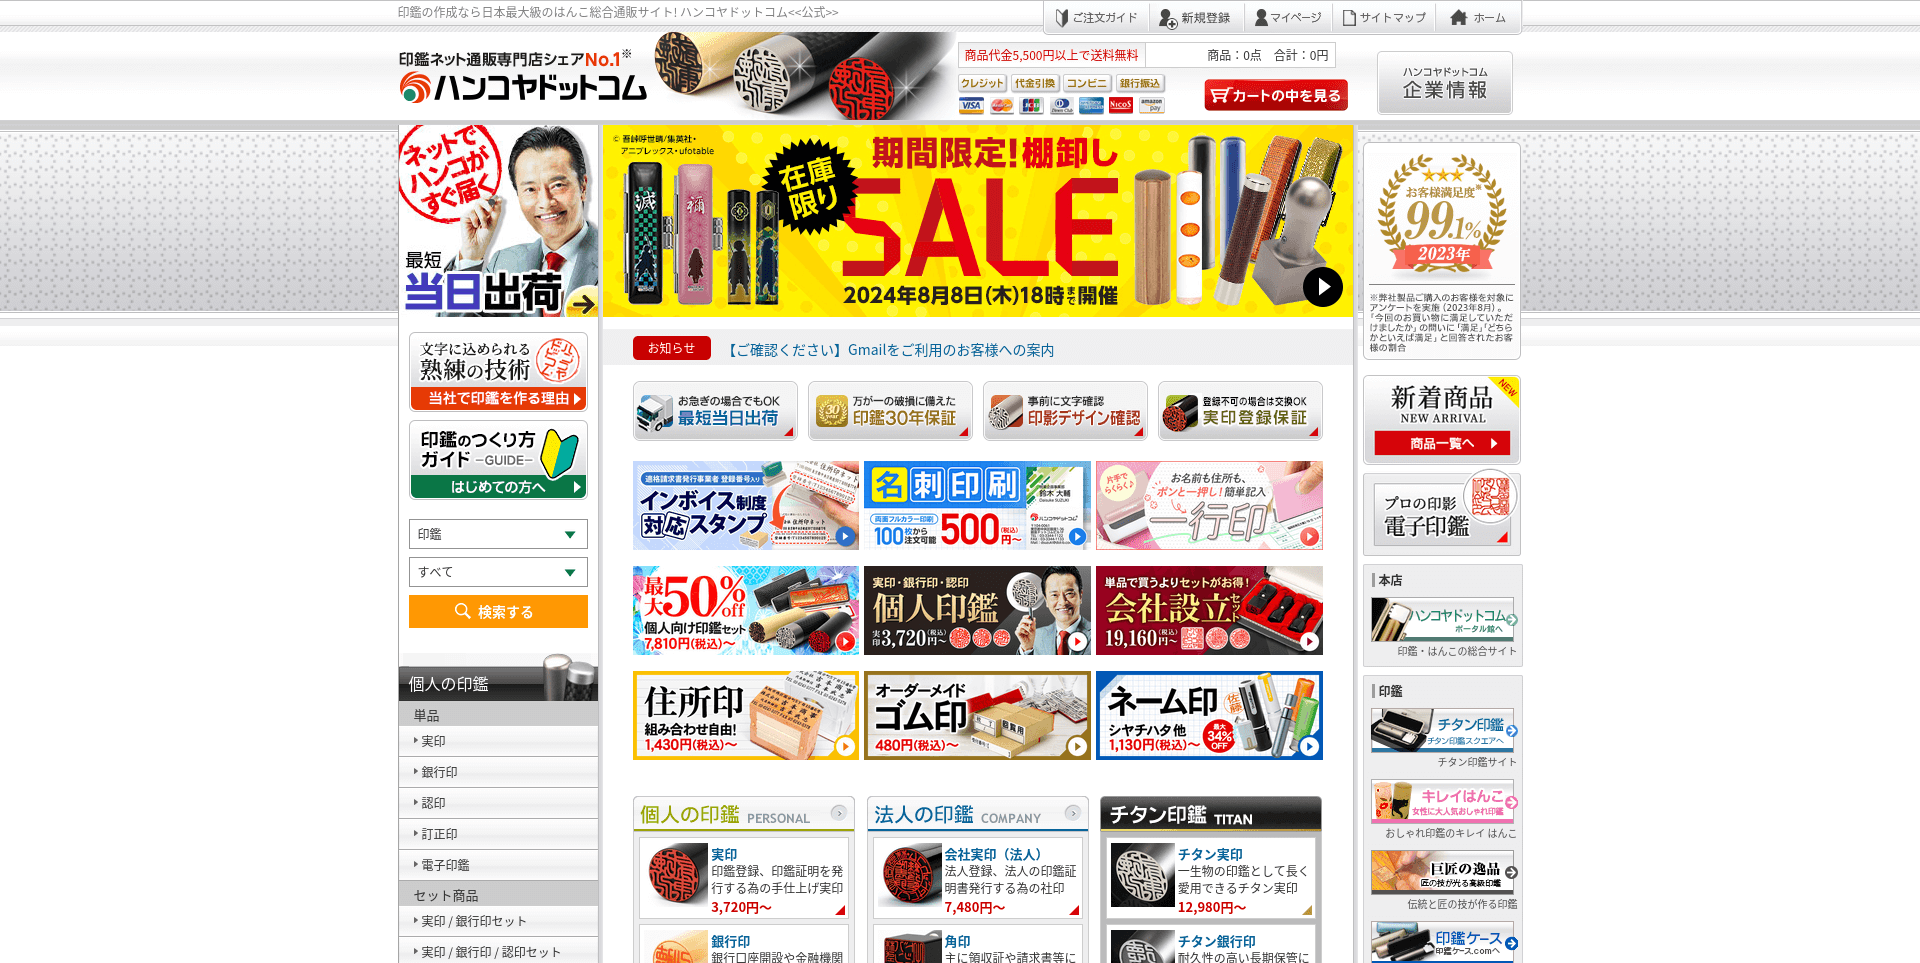
\includegraphics[width=\linewidth]{figures/hankoya.png}
      \caption{A specialist retailer's website, aiming for convenience through information density, showcases a historical device still in use for administrative processes in Japan: stamps~\cite{Ha24}.}
      \label{fig:hanko}
    \end{subfigure}
    \hspace{0.025\textwidth}
    \begin{subfigure}{0.45\textwidth}
      \centering
      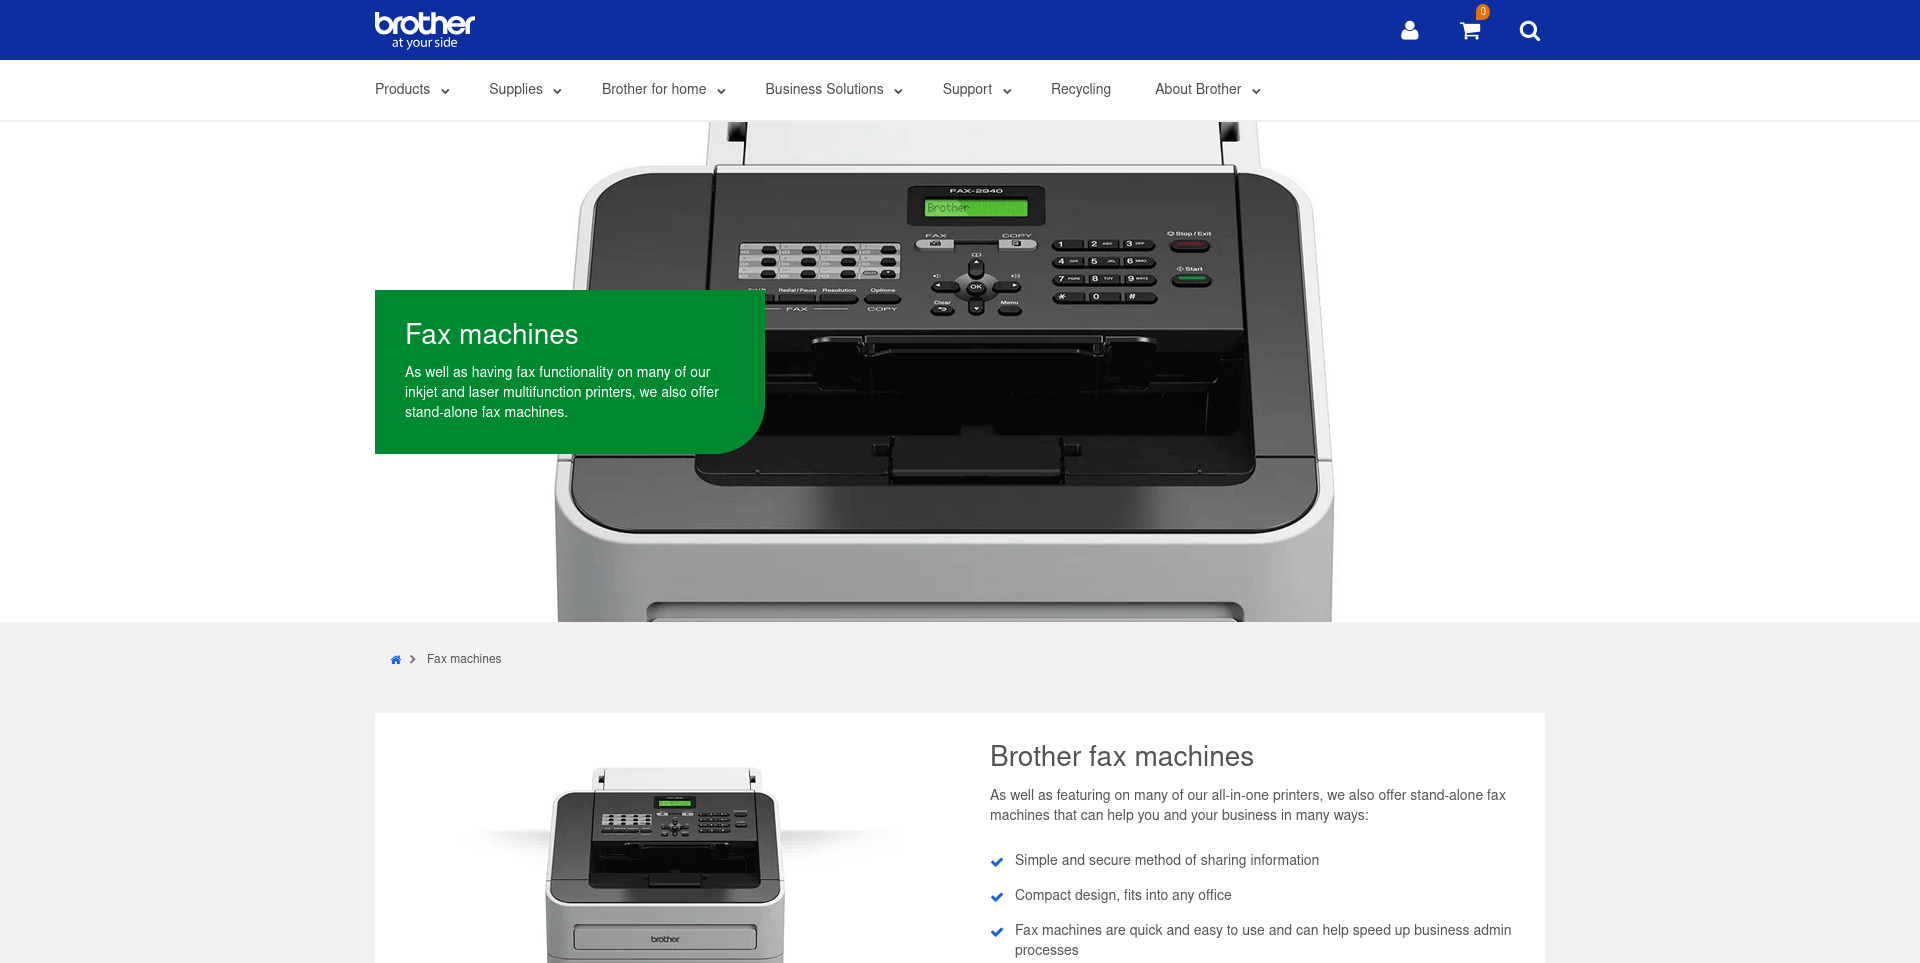
\includegraphics[width=\linewidth]{figures/brother.png}
      \caption{A specialist retailer's website, aiming for convenience through cleanliness, showcases a historical device still in use for administrative processes in Germany: fax machines~\cite{Br24}.}
      \label{fig:fax-machine}
    \end{subfigure}
    \caption{Introductory example for differences in web design.}
    \label{fig:intro-examples}
\end{figure}

While Western websites often use whitespace to create a clean, focused appearance, Japanese culture values high information density on each page as a form of convenience and perceived control.
This observation is reflected in the epigraph preceding this chapter.


\subsection{Research Question}
\label{sec:intro-research-question}

Building on the background provided in the previous section, the primary research question guiding this thesis is:

\begin{enumerate}
    \item[] \Question{rq:0}{Can we test or refute hypotheses on global variations in website code?}

    Our expectation is that such global variations can be detected and analyzed using a Big Data pipeline specifically created for this purpose.
    However, several factors could complicate the results or, in the worst case, make them unattainable.
    These factors include potential issues such as selecting a suboptimal dataset for ingestion, which might contain insufficient meaningful information, challenges in technical implementation, or possible ambiguities in the results.
    Additionally, the variations sought in this research may diminish or even disappear over time as globalized standards, like universal code styles, find worldwide application across projects.

    To address the broad primary research question stated above, the following sub-questions are of implicit interest:

    \item[] \Question{rq:1}{What influence does culture have on code?}

    The motivation for this thesis is rooted in the intuition that human culture influences how code is written.
    This question aims to establish the general context for the study.
    If no cultural influence on code exists, our intuition would be incorrect—an outcome that should always be considered a possibility.
    Such a finding would still allow for the existence of global code variations; these variations would simply not be related to cultural differences, allowing the research to continue even if the initial assumption is disproven.

    \item[] \Question{rq:2}{Which global variations in code have been researched before?}

    This practical question about the scientific context aims to ensure that this thesis provides highest academic benefit by avoiding redundancy with previous efforts.
    Additionally, referencing variations identified in prior research allows for validation checks on our findings through benchmarking comparison.
    Finally, understanding the extent of existing research into this topic helps determine whether further theoretical or practical results would be beneficial to the current scientific community.
    The answer to this question should yield two primary insights, guiding the focus of the following chapters, which are articulated as subquestions below.

    \begin{enumerate}
        \item[] \subQuestion{rq:21}{Which specific feature patterns in website code can be identified and analyzed for global variations?}

        This thesis is intended as foundational work that can support future expansions in global web analysis.
        Although this study primarily focuses on \ac{html}, other aspects of websites should be examined to reach holistic conclusions on global code variations.
        Analysis could range from measuring document sizes to timing web resource connection speeds.
        Defining a scope of feature patterns to analyze clarifies which areas remain open for future research.

        \medskip
        \item[] \subQuestion{rq:22}{Which statistical methods and algorithms are effective in detecting global variations in website code?}

        Assuming the pipeline design successfully processes data as specified by our objectives in \cref{sec:intro-objectives}, an evaluation of the resulting data is necessary to draw meaningful conclusions.
        It is therefore essential to make an informed decision on which evaluation methods or algorithms to use for optimal results.
    \end{enumerate}

    \item[] \Question{rq:3}{Which data sources can be used to yield valuable insights?}

    After clarifying cultural influences on code and previous research, it is necessary to identify data sources that support the research.
    To cater to varying interests among fellow researchers, this question is divided into two sub-questions: one addressing publicly available data and another considering private data sourcing.
    To stay focused on the primary research question, the topic of private data sourcing is discussed in an advisory manner, to avoid potentially confusing diversions from the main topic.

    \begin{enumerate}
        \item[] \subQuestion{rq:31}{Which datasets include the feature patterns under study and are publicly available?}

        Selecting suitable datasets increases the likelihood of producing actionable results.
        Additionally, the answer to this question may clarify the need for flexible ingestion of various data formats, as data archives might store websites in compressed formats rather than in their original state.
        Finally, utilizing publicly available datasets allows for reproducibility of this thesis's findings.

        \medskip
        \item[] \subQuestion{rq:32}{In which ways can useful datasets be sourced independently?}

        One may opt to source data independently to reduce reliance on external data providers or to analyze specific features that are not part of a publicly available dataset.
        While manually fetching features one by one is inefficient, knowledge of automated data-sourcing methods can be an advantageous addition to one's toolkit.
    \end{enumerate}

    \item[] \Question{rq:4}{What is the current state of Big Data and data engineering?}

    This question establishes a foundation for two more detailed questions on modern Big Data pipelines.
    Understanding the evolution of Big Data is essential for contextualizing how data pipelining fits within the broader field of data engineering.

    \begin{enumerate}
        \item[] \subQuestion{rq:41}{What constitutes a modern Big Data pipeline design?}

        Big data analyses are increasingly popular as datasets of substantial size become accessible to the public.
        Google Trends data show that global searches for ``big data'' began to rise around 2011 and peaked in 2017, as shown in \cref{fig:trends-big-data}.
        Similarly, \cref{fig:trends-data-pipeline} illustrates that worldwide searches for ``data pipeline'' increased in 2016 and have since trended upwards.

        \begin{figure}[H]
            \centering
            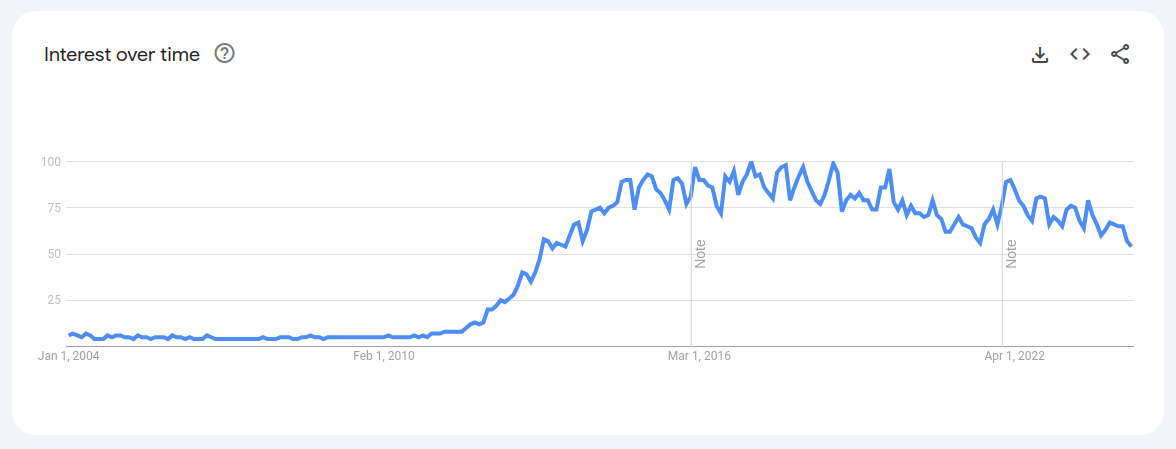
\includegraphics[width=\textwidth]{figures/trends-big-data.png}
            \caption{Google Trends data for worldwide searches of the term ``big data'' from 2004 to the present~\cite{Go2024}.}
            \label{fig:trends-big-data}
        \end{figure}

        \begin{figure}[H]
            \centering
            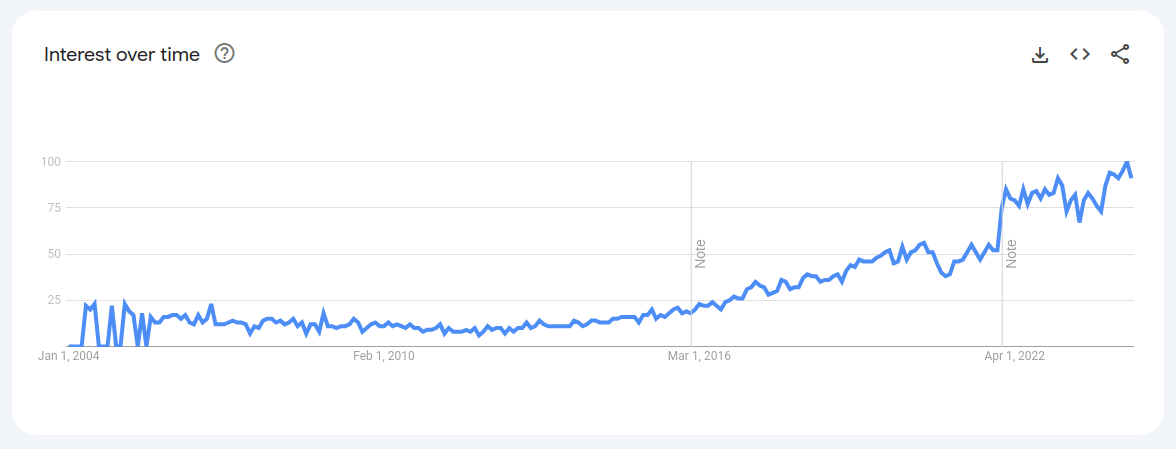
\includegraphics[width=\textwidth]{figures/trends-data-pipeline.png}
            \caption{Google Trends data for worldwide searches of the term ``data pipeline'' from 2004 to the present~\cite{Go2024}.}
            \label{fig:trends-data-pipeline}
        \end{figure}

        From these trends, it can be concluded that Big Data pipeline design remains an area of active development, in which universally agreed-upon standards might not yet exist.
        The pipeline designed in this thesis should prioritize support for the most promising advancements in Big Data pipeline research over commercial usefulness.

        \medskip
        \item[] \subQuestion{rq:42}{How can the effectiveness and accuracy of the pipeline be benchmarked?}

        This question is intended to be addressed only briefly in this thesis, as it represents a potential topic for future in-depth research.
        However, the work in this thesis will establish a foundation for a qualitative evaluation of the findings.
        Through a thorough literature review, methods will be identified to sufficiently validate the pipeline's effectiveness and accuracy, aiming to support a clearer interpretation of the results' significance.
    \end{enumerate}
\end{enumerate}

These questions aim to explore the core hypothesis of this thesis, guiding the design, implementation, and analysis of the proposed data pipeline system.


\subsection{Objectives}
\label{sec:intro-objectives}

Complementary to the theoretical foundation laid out in \cref{sec:intro-background-and-motivation} above, the primary practical aim of this thesis is to develop a scalable data pipeline capable of ingesting, processing, and analyzing website code from around the world.
The pipeline design should adhere to contemporary data engineering methodologies, enabling large volumes of data to flow smoothly.
These are our objectives:

\begin{enumerate}
    \item \textbf{Design and implement a scalable data pipeline}

    The system should be capable of handling diverse data formats and allow for flexible incorporation of additional data sources in the future.
    While \ac{html} is the primary candidate for analysis due to its accessibility, the pipeline should not be restricted to specific data formats or programming languages.
    Instead, it should accommodate any machine-readable data related to websites, including both well-structured sources, such as Common Crawl, and less-structured data, like transmission logs or potentially incomplete data such as the initial bytes of a website's HTML code.
    Additionally, the pipeline design should aim to use storage space as efficiently as possible.
    The pipeline should enable:

    \begin{enumerate}
        \item ingestion of diverse data sources, including both well-structured and less-structured data,
        \item transformation, analysis, and visualization of key metrics to yield insightful results, and
        \item persistence of ingested data and derivatives with minimal compute and storage usage.
    \end{enumerate}

    \item \textbf{Identify and quantify global variations in website code}

    Following the implementation and operation of the system, a visualization tool should be selected and configured to effectively represent the data returned by the pipeline.
    The visualizations provided should assist in interpreting and understanding the analysis results.

    \item \textbf{Evaluate the qualitative performance of the data pipeline}

    Assess the accuracy and reliability of the proposed system in detecting and analyzing global variations in website code, including evaluating the precision of variation detection and the system's ability to handle datasets at scale.
    The central outcome of all data processing, analysis, and evaluation efforts should be the capacity to confidently identify feature patterns that exhibit global variations.

    \item \textbf{Formalize a data ingestion module definition}

    Finally, this thesis will provide guidelines for future research that the pipeline will facilitate.
    These guidelines will enable researchers to incorporate additional data sources, refine analysis techniques, and enhance system performance, thereby contributing to ongoing research in this field.
\end{enumerate}

\subsection{Thesis Structure}
\label{sec:intro-thesis-structure}

This thesis is organized into chapters that progressively build a comprehensive understanding of the research and its findings.
Following the introduction provided in this chapter, the next chapter covers important related work, reviewing existing literature on cultural dimensions, global variations in website code, Big Data, and data engineering.
It establishes the context for the research and identifies the gaps addressed by this thesis.

With a clear scope established, the third chapter outlines the intended system design.
It describes the intuitive approach and details the composition of the data pipeline, including the processes of extracting, loading, and transforming data, as well as visualization strategies.

Chapter four moves on to the implementation phase, detailing the practical steps taken to set up the storage and compute infrastructure, as well as the pipeline's ingestion, transformation, and visualization layers.
It also explains how \ac{dx} is ensured and how the overall system is deployed to production.

The fifth chapter presents the analysis and results.
It showcases several graphs that provide insight into the processed dataset and reports on the pipeline's performance, \ac{dx}, and perceived reliability during operation.

In the sixth chapter, the focus shifts to evaluating the results.
This includes discussions on the implications of the findings, study limitations, potential biases, and the scalability and extensibility of the system.

The seventh chapter explores future work, suggesting directions for further research as well as potential improvements to the system.
Possible extensions, optimizations, and replacements for several parts of the pipeline are suggested to enhance the pipeline's flexibility.

Finally, the eighth chapter concludes this thesis by summarizing its contributions and findings and reflecting on the relevance of the research to the fields of Big Data and web development.


\newpage
\acresetall
\cleardoublepage
\section{Related Work}
\label{section:rw}
%
\lipsum


\newpage
\acresetall
\cleardoublepage
\section{Design}
\label{sec:design}

\epigraph{
    ``To keep up, our mental models of the world must adapt to new data, some of which contains new dimensions - new ways of seeing things we had no conception of before.''
}{
    Yavuz et al.~\cite{Yavuz2019}
}

This chapter outlines the design of the system developed to analyze global variations in website code.
The design is driven by the need to address the primary research question: Can we test or refute hypotheses on global variations in website code?
To achieve this, the system must be scalable, flexible, and capable of handling large volumes of diverse data sources.
This chapter is structured according to the specific objectives and sections outlined in the table of contents, providing a detailed technical specification of the system.

\subsection{Prerequisites}
\label{sec:design-prerequisites}

The technical infrastructure provided by the academic institution is a Kubernetes cluster\footnote{A cluster is a network of machines.}.
The cluster consists of 18 nodes\footnote{Nodes are machines in a network.} with a combined 240 \ac{cpu} cores, 3.69~TB of \ac{ram}, and approximately 77.1TB of \ac{ssd} storage capacity.
A \href{https://www.rancher.com/}{\textit{Rancher}} \ac{gui} provides access to visual resource management and monitoring.

\subsubsection{Intuitive Approach}
\label{sec:design-prerequisites-intuitive-approach}

\Cref{fig:design-intuitive-approach-services} shows an initial mockup of the service architecture.
In the top left, the mockup illustrates three exemplary data sources: \ac{http} data from Common Crawl, \ac{html} data from the \href{https://archive.org/}{\textit{Internet Archive}}, and partial \ac{html} data stored on storage media in the German city of \textit{Jena}.
All data is ingested by a \textit{Link Finder} service, which stores its results in a \href{https://www.mongodb.com/}{\textit{MongoDB}} database (shown at the bottom).
The \texttt{Link[]} output of the Link Finder is then passed to a \textit{Link Matcher} service and subsequently to a \textit{Group} service.
The intermediate storage for these last two services is a \href{https://clickhouse.com/}{\textit{ClickHouse}} database.
For a decoupled service architecture, Kafka is used as a real-time event streaming platform, enabling services to respond to data changes.
This design assumes that each service progressively reduces the size of the processed data.

The second mockup, shown in \cref{fig:design-intuitive-approach-branching}, visualizes a data branching concept where actors build data transformation sequences with partially shared intermediate results in \acp{dag}.
For example, the green actor \textit{Jonas} uses the central \textit{HTTP} dataset, feeding into a \textit{Link 1} service and subsequently a \textit{CoreJS} service.
A blue actor \textit{Adrian} mostly follows the same sequence but diverges to a \textit{Link 2} service in the last step.
This mockup illustrates an example transformation flow of a base dataset that includes \ac{css}, \ac{js}, and \ac{html} data, from which links are extracted and either checked for a target in a \ac{cdn} hosting the \href{https://github.com/zloirock/core-js}{\textit{core-js}} library or processed differently.
This branching concept is inspired by the branching structure of the \ac{vcs} \href{https://git-scm.com/}{\textit{Git}}.
Shared datasets minimize duplication in computation and storage, thus enhancing efficiency.

\begin{figure}[H]
    \centering
    \begin{subfigure}{.45\textwidth}
      \centering
      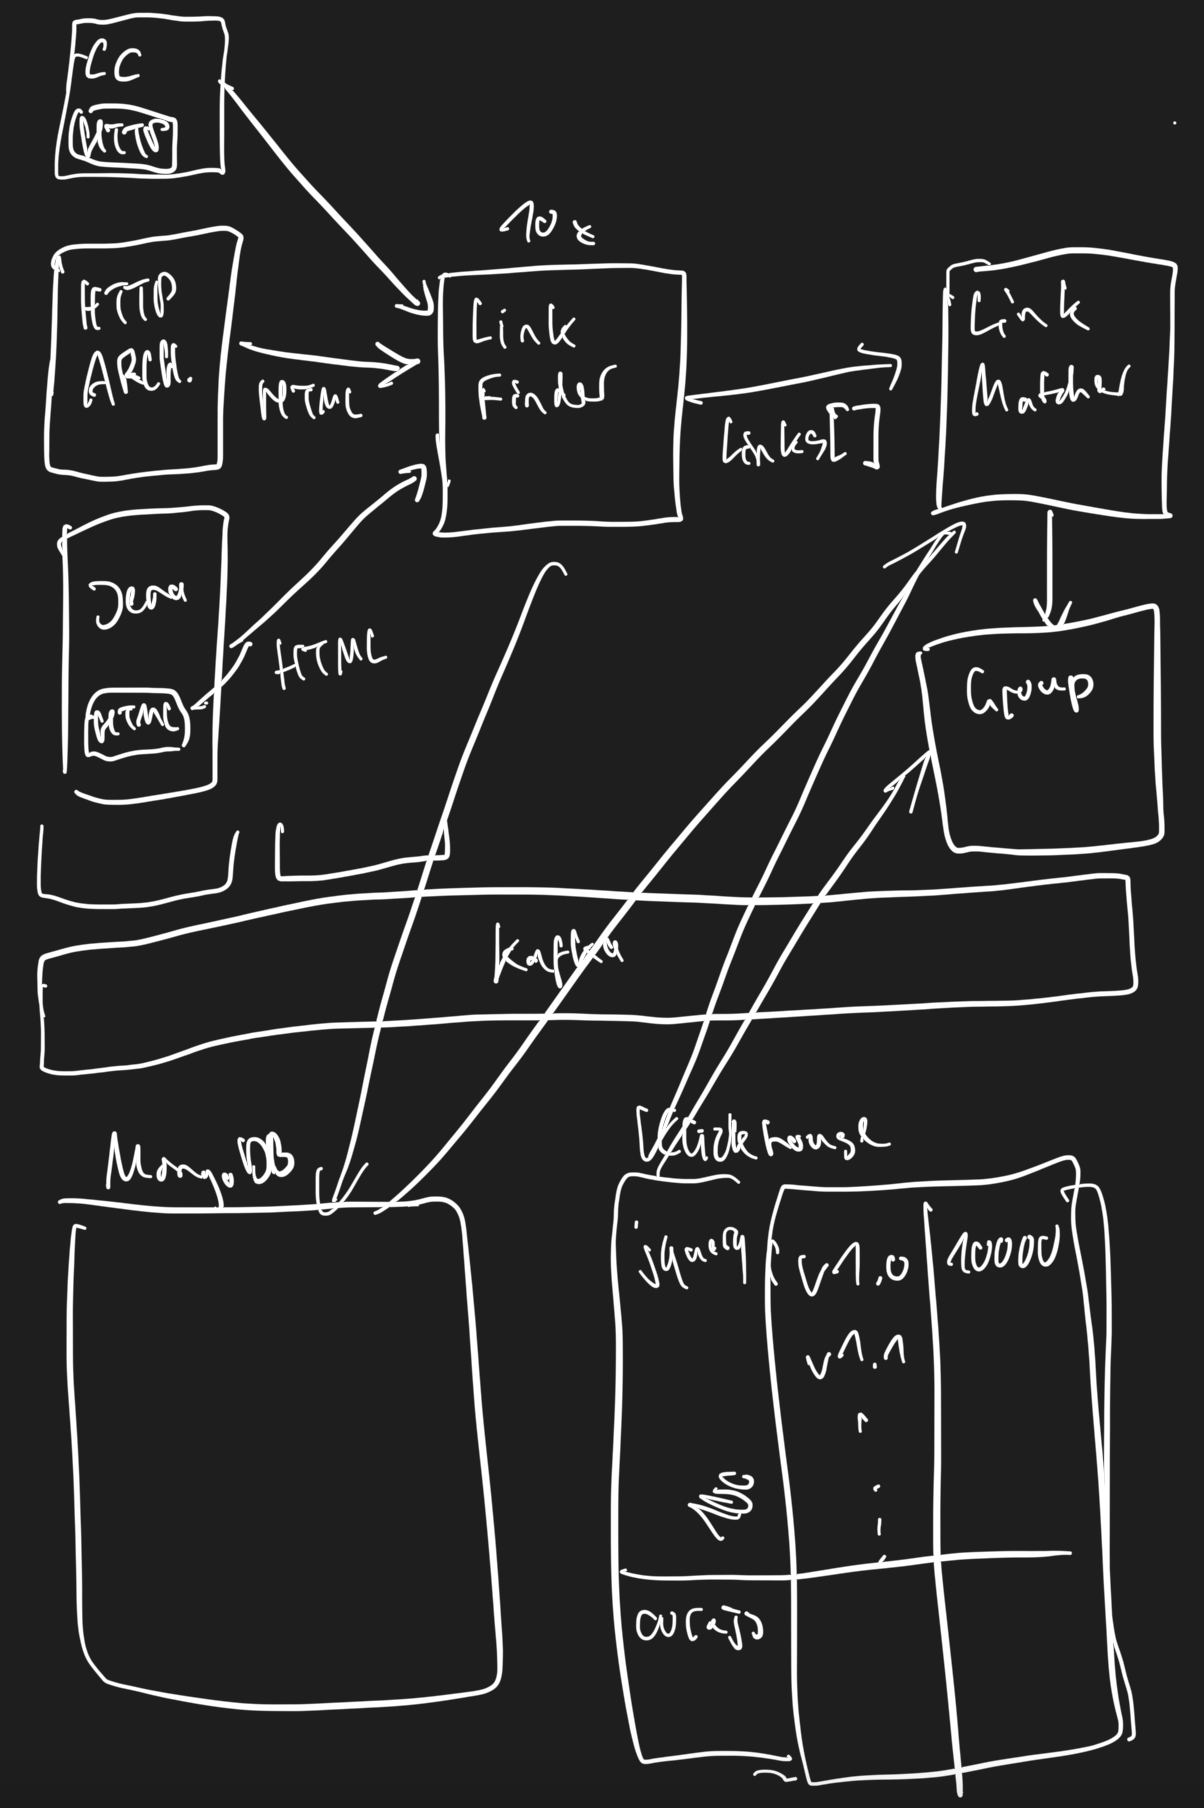
\includegraphics[width=\linewidth]{figures/approach-services.png}
      \caption{The pipeline's service architecture.}
      \label{fig:design-intuitive-approach-services}
    \end{subfigure}
    \hspace{0.05\textwidth}
    \begin{subfigure}{0.45\textwidth}
      \centering
      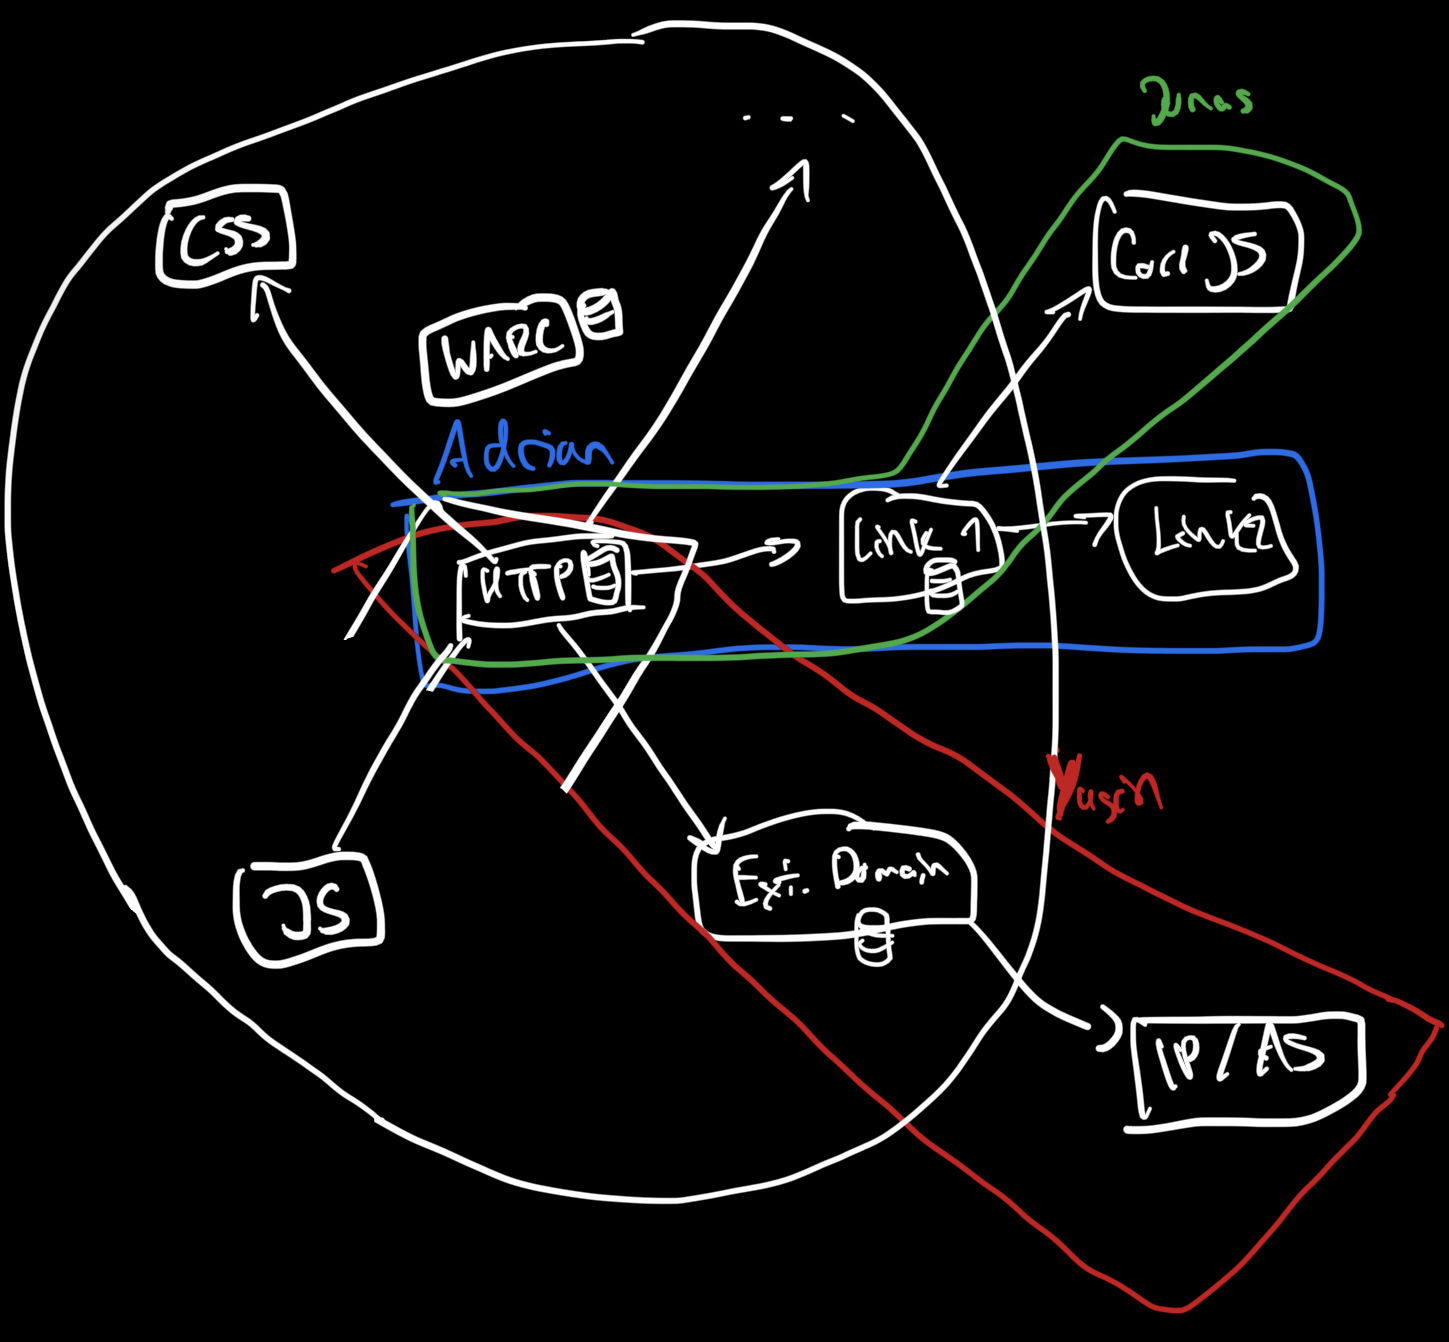
\includegraphics[width=\linewidth]{figures/approach-layered.png}
      \caption{The pipeline's data branching.}
      \label{fig:design-intuitive-approach-branching}
    \end{subfigure}
    \caption{Initial draft mockups.}
    \label{fig:design-intuitive-approach}
\end{figure}


\subsubsection{Storage}
\label{sec:design-storage}

In a distributed system, i.e., a system consisting of multiple nodes that collectively provide compute and storage resources, a key challenge is to maintain the technical guarantees of individual components when they operate within a networked environment.
A typical consumer-grade computer manages storage independently: files are saved to and retrieved from storage media directly connected to that machine.

In more complex systems with multiple nodes, a storage medium containing some data may not be physically connected to the machine requesting access to it.
Additionally, data that exceeds a single storage medium's capacity should be stored across multiple storage devices.
Storage management software, therefore, must handle reading and writing data distributed across nodes and storage media, which may only communicate via a network.

For Kubernetes, which serves as the foundational infrastructure, \href{https://longhorn.io/}{\textit{Longhorn}} provides a block storage solution.
Understanding Longhorn's distributed storage concept is fundamental, as it is the provisioned storage system in the Kubernetes cluster.

\begin{figure}[H]
    \centering
    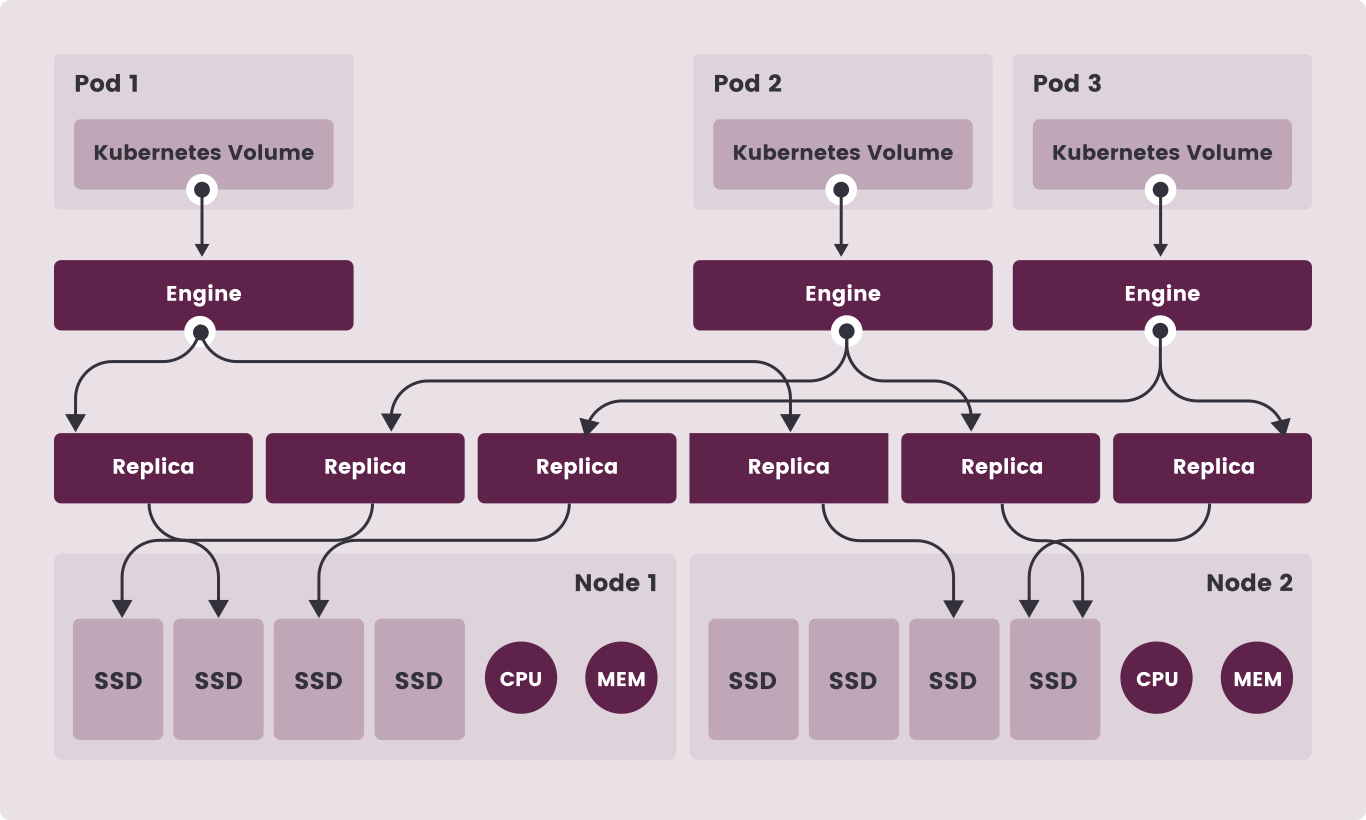
\includegraphics[width=\textwidth]{figures/longhorn.png}
    \caption{Longhorn's storage system~\cite{LonghornAuthors2024}.}
    \label{fig:longhorn}
\end{figure}

\Cref{fig:longhorn} illustrates the Longhorn storage system.
In simple terms, Longhorn enables the creation and usage of virtual storage volumes that span multiple physical storage media and nodes.
To ensure high availability and data integrity—even in the event of individual node failures—data fragments are replicated across multiple locations.
If a node fails, Longhorn automatically recreates the unavailable data replicas on other active nodes.
Longhorn also includes a snapshot-based backup functionality.

In summary, data written to Longhorn-managed storage is divided into fragments and redundantly stored across different nodes.
This fragmentation and distribution impacts the performance of computations involving the data.
If data were stored on a single distinct node, computations should ideally be conducted on a \ac{cpu} close to that node to minimize slow data transfers.
Since multiple copies of the data are spread across available nodes, however, we can generally assume that data will be accessible quickly enough\footnote{See \cref{sec:future-work-optimizations} for a potential optimization using node affinity in Kubernetes.} for computations on any node, especially considering the ease of use that Longhorn provides.

If Longhorn were not a prerequisite, it would be worth considering \acp{dfs} like \textit{Ceph}, \textit{GlusterFS}, and particularly \ac{hdfs} (the Hadoop Distributed File System).
\ac{hdfs} is a file system designed for the Hadoop project, which supports distributed computing and is promoted as a system that ``scales up from single servers to thousands of machines, each offering local computation and storage''~\cite{ASF2024b}.
Research suggests that Hadoop may be able to guarantee data locality for computational tasks.
However, placing a file system with strong data locality guarantees on top of a block storage solution with weaker guarantees, such as Longhorn, would not yield significant advantages, as the underlying system's limitations would constrain overall data locality.

In this setup, without a strict commitment to Hadoop, we retain the flexibility to choose a suitable data format, provided it is compatible with \texttt{\ac{ext4}} on a Kubernetes volume claim provisioned by Longhorn.


\subsubsection{Databases}
\label{sec:design-databases}

In the context of Big Data, \ac{olap} is more relevant than \ac{oltp} as processing large quantities of data quickly takes precedence over strict \ac{acid} guarantees.
\ac{olap} systems often use a columnar storage format, which allows for distributed execution of aggregate functions, such as calculating the minimum, maximum, average, or sum of a large dataset's numeric property.

Consider a table like \cref{tab:result-example} that stores millions of website \acp{url}, each with a country assignment and detected technologies.
For example, we might want to find the average number of web technologies used.
In a row-oriented \ac{oltp} database, each row would need to be loaded and scanned for the \texttt{web\_technology\_count} value, often passing over irrelevant columns.

\begin{table}[H]
    \centering
    \begin{tabular}{|c|c|c|c|c|}
    \hline
    \textbf{url} & \textbf{country} & \textbf{web\_technologies} & \textbf{web\_technology\_count} & \textbf{…} \\
    \hline
    https://example.jp & Japan & AMP, Google Analytics & 2 & … \\
    \hline
    \end{tabular}
    \caption{Row-oriented storage format in an OLTP system.}
    \label{tab:result-example}
\end{table}

In a columnar \ac{olap} database, values of interest can be loaded as a distinct dataset, as shown in \cref{tab:olap-example}, which allows for efficient aggregate calculations.
Here, the average of the \texttt{web\_technology\_count} is \texttt{1}.

\begin{table}[H]
    \centering
    \begin{tabular}{|c|}
    \hline
    \textbf{web\_technology\_count} \\
    \hline
    2 \\
    \hline
    0 \\
    \hline
    1 \\
    \hline
    … \\
    \hline
    \end{tabular}
    \caption{Column-oriented storage format in an OLAP system.}
    \label{tab:olap-example}
\end{table}

Another benefit of columnar storage is the potential for compression due to repetitive data patterns.
\Cref{tab:compression-example} shows an example where data, as queried on the left, could be stored more efficiently in compressed form on the right.
In simple terms, column serialization can store a value once and remember where to repeat it instead of duplicating the value.
For instance, adding a \texttt{dataset\_id} column to \cref{tab:result-example} where every record holds the same value (e.g., \texttt{CC-MAIN-2024-42}) would require minimal storage due to compression.

\begin{table}[H]
    \centering
    \begin{tabular}{|c|}
    \hline
    \textbf{country} \\
    \hline
    Germany \\
    \hline
    Germany \\
    \hline
    Germany \\
    \hline
    … \\
    \hline
    \end{tabular}
    \begin{tabular}{|c|}
    \hline
    \textbf{country} \\
    \hline
    Germany*3 \\
    \hline
    \\
    \hline
    \\
    \hline
    … \\
    \hline
    \end{tabular}
    \caption{Simplified example of view (left) and compression (right) in columnar storage.}
    \label{tab:compression-example}
\end{table}

An in-memory representation of such a columnar format is provided by \textit{Apache Arrow}, enabling support for \ac{simd} operations in modern processors.
Arrow aims to create a standard across databases and programming languages, enhancing interoperability and minimizing the need for custom serializations.
Systems such as the distributed compute engine Spark, the \ac{olap} \ac{dbms} ClickHouse, and dataframe libraries like Pandas and Polars, as well as the Apache Parquet file format, use Arrow.

An optional prerequisite in the \ac{olap} context is ClickHouse, as an instance of this solution is already provisioned in the university's Kubernetes cluster.
The \href{https://altinity.com/kubernetes-operator/}{\textit{Altinity Kubernetes Operator for ClickHouse}} simplifies the management of ClickHouse installations on Kubernetes.
However, as noted by Zhang and Dai, ClickHouse's strong coupling of storage and compute nodes poses risks to cluster stability~\cite{Zhang2023}.

ClickHouse uses the \ac{osi}-approved \textit{Apache License 2.0} open source license and is optimized for real-time analytics.
It is important to note that data freshly inserted into ClickHouse might not be immediately available for queries due to insert buffering and background merging for data compaction, as ClickHouse prioritizes fast query execution over strict data consistency.

Although real-time capabilities are out of scope for our Big Data pipeline design, ClickHouse provides an informative benchmark for analytical \acp{dbms} called \href{https://benchmark.clickhouse.com/}{\textit{ClickBench}}.
This benchmark evaluates the performance of 42 queries across 69 database systems (or configurations) on various machine or cluster sizes.
Metrics for data load time, storage size, as well as cold and hot run performance, are also provided for comparison.

For this thesis, the following \ac{olap} systems were selected for closer inspection based on an extensive search for popular solutions: ClickHouse, \href{https://doris.apache.org/}{\textit{Apache Doris}}, \href{https://druid.apache.org/}{\textit{Apache Druid}}, \href{https://pinot.apache.org/}{\textit{Apache Pinot}}, and \href{https://starrocks.io/}{\textit{StarRocks}}.
Additional noteworthy mentions include:

\begin{itemize}
    \item \href{https://snowflake.com/}{\textbf{Snowflake}}, which achieves minimal storage size but is only available as a hosted cloud service with credit-based pricing, based on virtual warehouse size and hours of compute;
    \item \href{https://clickhouse.com/chdb}{\textbf{chDB}} and \href{https://duckdb.org/}{\textbf{DuckDB}}, which function as in-process engines similar to what \href{https://www.sqlite.org/}{\textit{SQLite}} offers for \ac{oltp};
    \item \href{https://motherduck.com/}{\textbf{MotherDuck}}, a hosted cloud service for DuckDB; and
    \item \href{https://postgresql.org/}{\textbf{PostgreSQL}} as a performance reference for an \ac{oltp} \ac{dbms}: PostgreSQL requires approximately 88 times the load time, 50 times the hot and cold run times, and ten times the storage size compared to each category's baseline.
\end{itemize}

ClickBench highlights individual challenges faced by Pinot and Druid.
For Pinot, the following observations are made:

\begin{quote}
    ``It successfully loaded only 94465149 out of 99997497 records.
    Some queries returned NullPointerException.
    The loading process is painful - splitting to 100 pieces required.
    It does not correctly report errors on data loading, the results may be incorrect.''~\cite{Milovidov2022}
\end{quote}

For Druid:

\begin{quote}
    ``Druid is killed and restarted after every query.
    Otherwise some queries make Druid degraded and results are incorrect.
    For example after Q13 even SELECT 1 works for 7 seconds.''~\cite{Milovidov2022}
\end{quote}

These observations, documented by Alexey Milovidov, led to the decision to exclude Pinot and Druid as database systems for the Big Data pipeline designed here.

This leaves us with Apache Doris and StarRocks.
Doris is notable for its straightforward architecture.
In contrast, Pinot and Druid rely on \textit{Apache Zookeeper} for service coordination, with Druid, in particular, requiring a complex architecture involving a coordinator, overlord, broker, historical, and middle manager services.
Doris, on the other hand, only requires frontend services for query planning, backend services for data execution, and a meta store for metadata management.

StarRocks is a fork of Doris, with licensing and trademarking challenges arising between the projects after the fork~\cite{Chen2024}.
Originally named \textit{DorisDB}, StarRocks initially used the \textit{Elastic License}, which disqualified it from open source designation due to restrictions on commercial use.
In 2022, however, StarRocks switched back to the Apache License 2.0, the same license Doris uses.
Both Doris and StarRocks support the Lakehouse architecture and the Iceberg table format.

Before discussing distributed computing, it is worth outlining another use case for querying: querying across multiple heterogeneous data sources.
Data systems that evolve over time often amass multiple data pools.
For instance, some data may be stored in an \ac{oltp} \ac{dbms} like PostgreSQL, while other data might reside in a cloud data warehouse like Snowflake or similar alternatives.
This chapter ultimately selects a storage solution as a design choice, which may complement existing data stores at the academic institution.
To integrate this data and make the results of this thesis available for future research, a system capable of querying across diverse sources is essential.
This is where \textit{Trino} becomes relevant.

Trino is a fork of a project commonly known as \textit{Presto}, originally developed at Facebook.
Similar to the StarRocks fork from Doris, there was some ambiguity around the ownership of \textit{PrestoSQL} (the rebranded fork) and \textit{PrestoDB} (the original project).
The name change to Trino resolved this issue~\cite{Traverso2022}.

However, the databases and query engines mentioned are unsuitable for the flexible transformations we aim to enable in our Big Data pipeline.
Beyond merely reading table results, it should be possible to perform arbitrary computations on the data and insert results back into the dataset.
Thus, a proper design for data computations must be defined.

\subsection{Envisioned Result}
\label{sec:design-envisioned-result}

The final output of our Big Data pipeline should be clear visual insights that simplify understanding a large dataset.
Since we are working with global data, choropleth maps provide an effective visualization format.
Choropleth maps display a geographic area in which regions are shaded according to a statistical value.
These maps are often used to present election results, with sub-areas shaded in the winning party's color.

\Cref{fig:choropleth} illustrates a choropleth map that could represent the output of the Big Data pipeline designed in this thesis.
It shows a world map with countries shaded based on a metric such as the number of websites attributed to each country.
The map could display the total number of websites processed, websites above a certain size, or websites containing specific technology, such as the \textit{Wordpress} blogging platform.
Choropleth maps also help identify potential data biases; for instance, if many countries in a continent like Africa are left unshaded, the dataset may contain a bias warranting further investigation.

\begin{figure}[H]
    \centering
    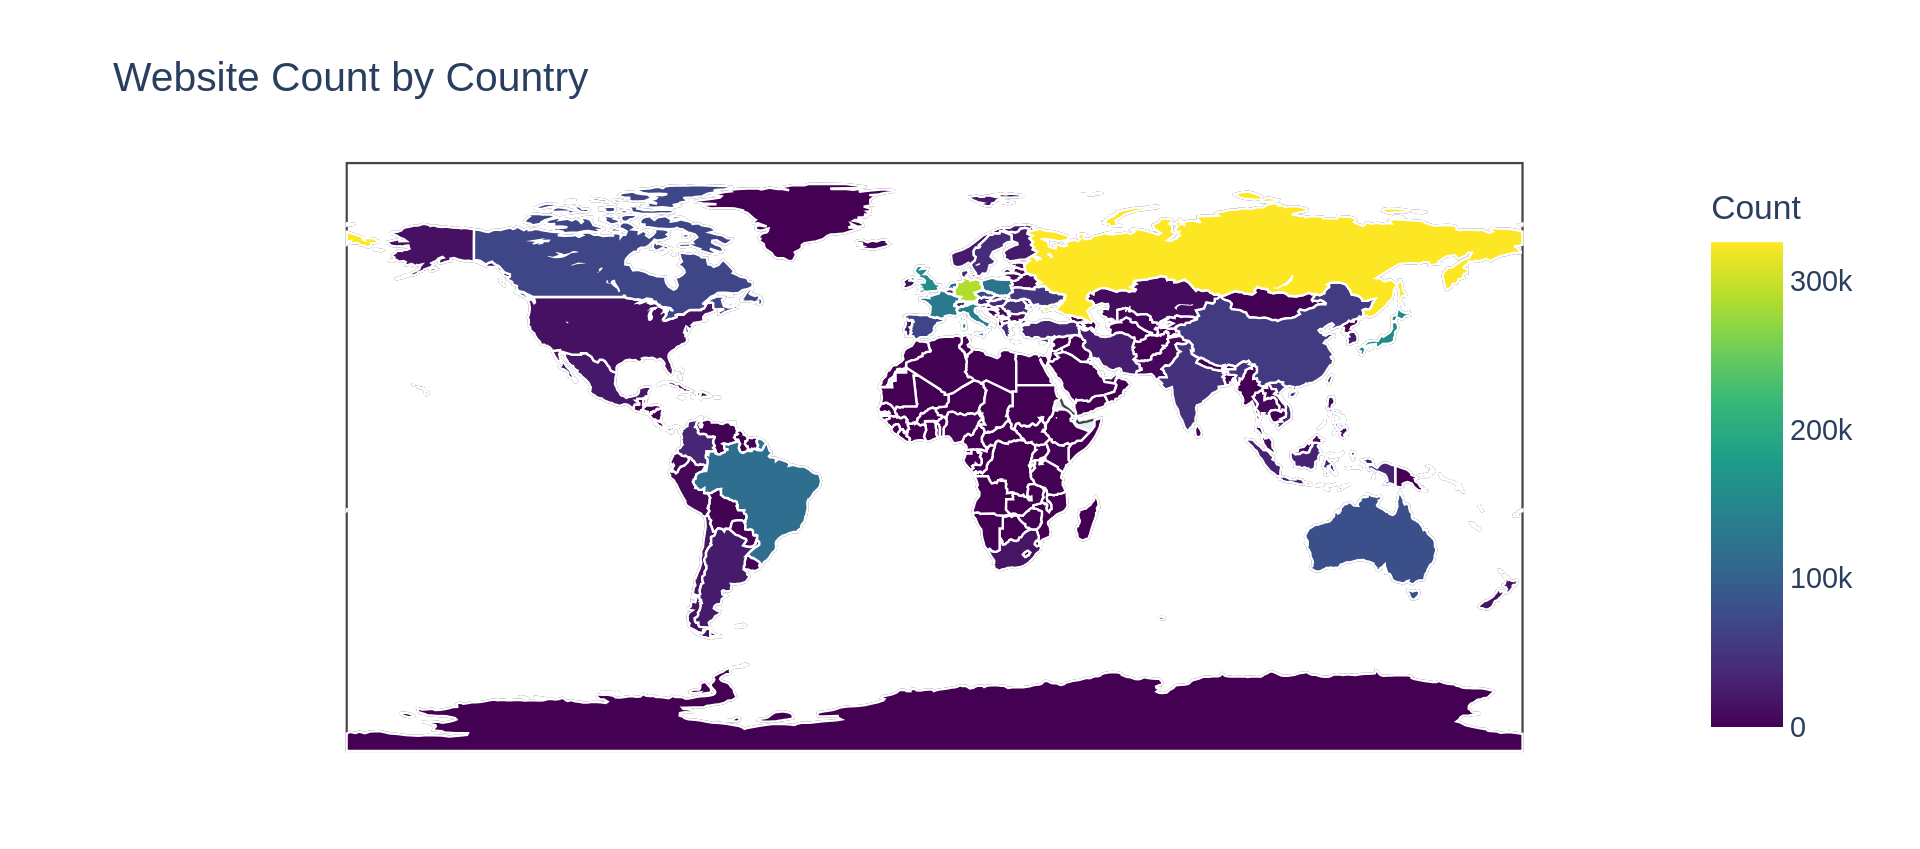
\includegraphics[width=\textwidth]{figures/charts/large/chart_fact_uri_choropleth.png}
    \caption{An example choropleth map showing the number of websites per country.}
    \label{fig:choropleth}
\end{figure}

The first design decision necessary is to determine how to attribute websites to specific countries.
Possible options include using the IP address of the website's host server, the address of a domain's owner, or the language of the text visible to website visitors.
However, because our top-down approach has delayed dataset selection, we are not yet certain which of these data types will be readily available.
Therefore, we choose to use part of a metric that is likely to be consistently accessible: a website's \ac{cctld}, such as \texttt{.de} in \texttt{https://example.de/page}.

A website's \ac{cctld} does not guarantee that its content is intended for citizens of the corresponding country or that it was created by residents of that country.
For example, \texttt{https://\-maev.si/} uses Slovenia's \ac{cctld} purely for a wordplay effect, while targeting German users.
Nevertheless, using the \ac{cctld} is sufficient for evaluating the capabilities of the Big Data pipeline.

Before proceeding to the next step, it is essential to remember that choropleth maps represent just one option for displaying results and should not restrict alternative methods of data interpretation.

Data visualization tools vary in their target user groups and feature sets.
Microsoft's \href{https://microsoft.com/power-platform/products/power-bi}{\textit{Power BI}} and Salesforce's \href{https://tableau.com/}{\textit{Tableau}} are designed primarily for corporate use cases.
These solutions are hosted by their providers, eliminating setup and maintenance costs for running the software on internal infrastructure.
However, as a result, these products are commercial offerings.
Both providers offer discounts for students and academic institutions.

Since internal infrastructure is already in place, as discussed in \cref{sec:design-prerequisites}, a lightweight alternative could be used to avoid dependency on external providers.

Open source solutions for data visualization include \href{https://superset.apache.org/}{\textit{Superset}} by the Apache Software Foundation and \href{https://redash.io/}{\textit{Redash}}, a community-driven project.
All of the tools mentioned so far enable the definition of connections to data sources, execution of queries against those data sources, and creation of dashboards that visually compose the results of these queries.
\Cref{fig:superset-dashboard} shows an example of a Superset dashboard, while \cref{fig:redash-query-editor} provides an example of the Redash query editor.

The main takeaway is that these tools offer interactivity, allowing visualizations to be defined and modified at runtime.
This feature-rich environment is beneficial for end users of data pipelines, such as data scientists.
However, this level of functionality also introduces complexity: for instance, Superset requires at least a metadata database, and for certain features, it also relies on a caching layer as well as a worker and beat service~\cite{ASF2024}.
This additional infrastructure is excessive for the non-essential part of the data pipeline design, especially since the visualization tools' data source support could become a limiting factor in upcoming storage decisions.
Nonetheless, it is important to be aware of these feature-rich solutions, as a solid data pipeline implementation could integrate these tools in future extensions.


\subsection{Decisions}
\label{sec:design-decisions}

Now that \cref{sec:design-prerequisites} has defined the prerequisites and \cref{sec:design-envisioned-result} has outlined our goal, we are able to make the necessary decisions to design the Big Data pipeline that meets the objectives defined in \cref{sec:intro-objectives}.
With Longhorn set as the storage solution, our first decision is to select a tool that enables complex distributed computations.
We then review our findings from \cref{sec:related-work-big-data-pipelines} on the characteristics of a modern Big Data pipeline and select a storage layout that fits our requirements.
With these two decisions in place, and with priority given to compatibility, flexibility, and popularity, the choice of programming language becomes straightforward.

These three foundational choices enable the systematic design of a data architecture within storage.
Finally, a modern \ac{gui} for managing workflows is selected.


\subsubsection{Compute}
\label{sec:design-compute}

As noted in \cref{sec:design-databases}, our dataset requires transformational computations that extend beyond simple querying.
For this purpose, the batch processing engine Spark offers a well-established and powerful open source framework for \ac{mpp}.
Spark's stream processing counterpart is Flink, although Spark also supports streaming in a limited form through micro-batching.
Flink graduated from Apache's incubation at the end of 2014, shortly after Spark completed its own graduation in February of the same year.

At its core, Spark utilizes \acp{rdd} for fault-tolerant distribution of immutable objects across a cluster's nodes without requiring redundant copies.
This approach is known as lineage-based fault tolerance.
If a partition of an \ac{rdd} is lost, Spark can recover it by tracing the lineage of transformations that created it.

In Scala and Java, these distributed objects can be manipulated via Spark's \textit{Dataset API}.
In Python and R, the \textit{DataFrame API} provides a similar structure, offering a dataset accessible through named columns.
The DataFrame API is also available in a row-based format for Scala and Java.
These \acp{api} provide comfortable abstractions for direct interaction with \acp{rdd}.

Spark performs computations in-memory, distinguishing it from disk-based processing frameworks like Hadoop, which executes the MapReduce model and writes results back to disk, generally making it slower than in-memory processing.

In the Hadoop MapReduce context, querying is facilitated by \href{https://hive.apache.org/}{\textit{Apache Hive}}, whereas Spark provides \textit{Spark SQL} as its native querying module, which also supports reading from Hive installations.

Other Spark modules include the \ac{ml} library \textit{MLlib} and \textit{GraphX}, an \ac{api} for graph-based computations.
Although these modules are not utilized in this thesis, they may be beneficial for future extensions.

A distributed Spark job involves three primary components:

\begin{itemize}
    \item \textbf{Drivers}, which initiate the software.
    \item \textbf{A master}, coordinating the executors.
    \item \textbf{Executors}, which handle their allocated portions of a job.
\end{itemize}

Spark can be deployed in either \textit{Client Mode} or \textit{Cluster Mode}.
In Client Mode, the Driver runs on the client machine that submits the job and must remain connected to the cluster to maintain the connection.
In Cluster Mode, the Driver operates on a worker node within the cluster, allowing the client to disconnect without impacting the job's execution.
\Cref{fig:spark-cluster} illustrates Spark's Cluster Mode, where Kubernetes, \href{https://mesos.apache.org/}{\textit{Apache Mesos}}, and \href{https://hadoop.apache.org/docs/current/hadoop-yarn/hadoop-yarn-site/YARN.html}{\textit{Apache Hadoop YARN}} are possible cluster managers.

\begin{figure}[H]
    \centering
    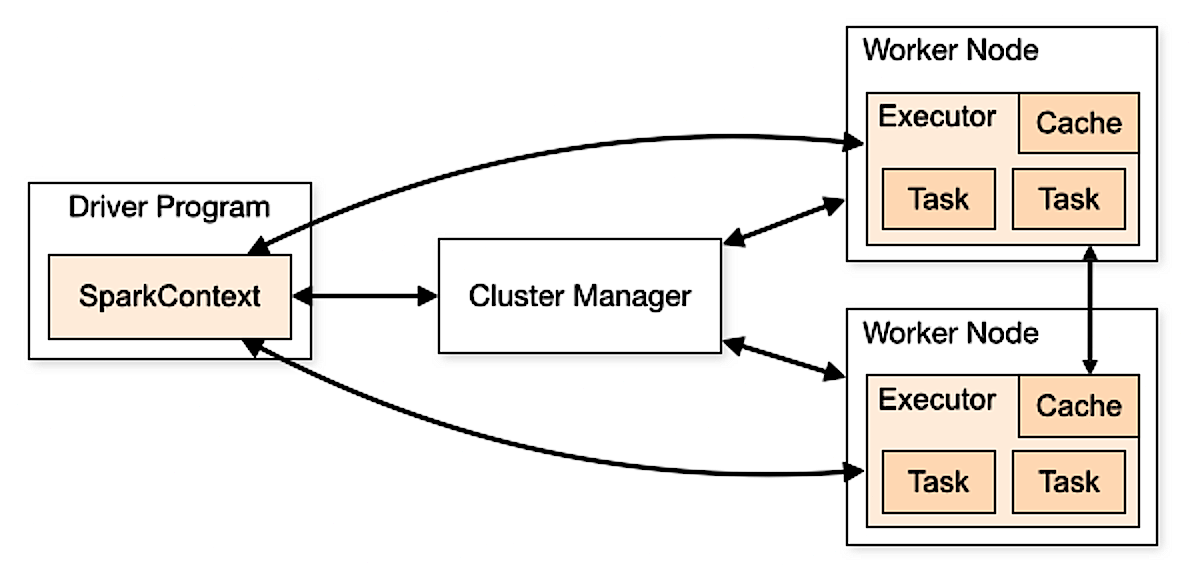
\includegraphics[width=0.75\textwidth]{figures/spark-cluster.png}
    \caption{Spark's architecture in cluster mode~\cite{ASF2024c}.}
    \label{fig:spark-cluster}
\end{figure}


\subsubsection{Data Format}
\label{sec:design-decisions-data-format}

We select an open table format because, with Spark as our distributed compute and query engine, we are not restricted to any format specific to a particular data management tool.
This decoupling aligns with the Lakehouse architecture.

There are three primary options for open table formats supporting the Lakehouse architecture:

\begin{itemize}
    \item \href{https://delta.io/}{\textit{\textbf{Delta Lake}}}, open-sourced in 2019 as part of the \href{https://www.databricks.com/}{\textit{Databricks}} ecosystem, later joined the Linux Foundation in 2020, reflecting a commitment to open governance and broader community development.
    \item \href{https://iceberg.apache.org/}{\textit{\textbf{Apache Iceberg}}}, open-sourced by \href{https://www.netflix.com/}{\textit{Netflix}} in 2018, was donated to the Apache Software Foundation in 2019, achieving top-level project status in 2020.
    \item \href{https://hudi.apache.org/}{\textit{\textbf{Apache Hudi}}}, open-sourced by \href{https://www.uber.com/}{\textit{Uber}} in 2017, became an Apache Incubator project in January 2019 and graduated to top-level project status in May 2020.
\end{itemize}

These tools vary in aspects such as Hudi's write optimization or external support, e.g., Iceberg is supported by Snowflake, whereas Hudi is not.
Fortunately, efforts have been made to simplify switching between formats or even using multiple formats simultaneously.
This flexibility is achieved by separating data files from metadata files.
Tools like \href{https://xtable.incubator.apache.org/}{\textit{Apache XTable}}\footnote{XTable was formerly known as \textit{OneTable} and was created by \href{https://www.onehouse.ai/}{\textit{Onehouse}}, a Lakehouse cloud provider.} and \href{https://www.databricks.com/product/delta-lake-on-databricks}{Delta Lake UniForm} convert metadata files across table formats while leaving data files unchanged.
However, certain tool-specific strengths, such as Hudi's write performance, may not be fully retained if Delta Lake is used as the foundation~\cite{Merced2024}.
An emerging real-time format for the Lakehouse architecture is \href{https://paimon.apache.org/}{\textit{Apache Paimon}}, though it is not yet as widely adopted as the previously mentioned solutions.

Another noteworthy tool is \href{https://projectnessie.org/}{\textit{Nessie}}, introduced by \href{https://www.dremio.com/}{\textit{Dremio}}.
Nessie, a transactional catalog, provides Git-like version control features for Iceberg Lakehouse storage.
With Nessie, it is possible to commit data changes transactionally across multiple branches without copying data.
This capability enables navigation through data history and parallel data versions, which was identified as a goal in \cref{sec:design-prerequisites-intuitive-approach} and illustrated in \cref{fig:design-intuitive-approach-branching}.
While Nessie will not be used in this thesis, researching it provided valuable insights into Iceberg, leading to the decision to use Iceberg as the open table format for the upcoming implementation.


\subsubsection{Programming Language}
\label{sec:design-decisions-programming-language}

The initial rationale for selecting TypeScript as the programming language for the Big Data pipeline, as outlined in \cref{sec:design-prerequisites-intuitive-approach}, was that those interested in website data analysis typically have experience in web development and are accustomed to TypeScript.
However, the research into Big Data, data engineering, and data science covered in \cref{sec:related-work-big-data}, along with the analysis of tools that best meet the targeted capabilities of the pipeline, points toward Python as the more suitable choice.

The design of a Big Data pipeline falls squarely within data engineering.
The primary objective of this thesis is to support future researchers by providing well-justified choices for tools that meet the goals defined in \cref{sec:intro-objectives}.
Specifically, the pipeline aims to assist researchers in exploring novel datasets and advancing scientific insights.
It is therefore essential to choose a programming language that offers robust integration within the data engineering ecosystem to avoid compatibility limitations and maintain flexibility in scientific applications.
This requirement suggests selecting a language that is both popular and extensively supported within the data engineering domain.

Python is a leading programming language across data engineering, data science, and artificial intelligence, and it ranked as the most popular language among coding learners in the 2024 \textit{Stack Overflow} developer survey~\cite{StackExchange2024}.
Python is also taught at the academic institution hosting this research.
Thus, selecting Python as the language for the Big Data pipeline will ensure broad accessibility for developers who will work with, extend, or integrate the system.

As discussed in \cref{sec:design-compute}, Spark provides a straightforward means of distributed computation for the pipeline's transformation stage.
Through \textit{PySpark}, it is easy to initiate Spark jobs in Python, offering strong alignment with the Python ecosystem.

TypeScript is also widely used, especially in web development, but it is less common in data-centric engineering fields.
TypeScript adds typing to \textit{ECMAScript} (commonly known as \ac{js}) and can be executed in environments like \href{https://nodejs.org/}{\textit{Node.js}}, \href{https://deno.com/}{\textit{Deno}}, or \href{https://bun.sh/}{\textit{Bun}}.
The main package ecosystem for \textit{ECMAScript} is the \href{https://www.npmjs.com/}{\textit{npm}} registry.
However, no actively maintained Spark client comparable to PySpark for Python could be found in npm.

Thanks to \textit{Apache Livy}, a \ac{rest} \ac{api} can be set up for Spark, enabling interaction with Spark from any language that supports \ac{http} requests.
Without Livy, establishing a Java socket server to act as middleware between the client and Spark would be necessary, along with a custom client implementation.
Nevertheless, the most widely documented method of interacting with Spark remains PySpark, further supporting Python as the optimal choice.


\subsubsection{\ac{elt}}
\label{sec:design-decisions-elt}

As shown in \cref{sec:related-work-big-data-pipelines}, a modern storage environment like Rancher allows for using the \ac{elt} step order instead of the \ac{etl} order in our pipeline.
This section explains our decisions on how extraction, loading, and transformation will be implemented.

With Python as the programming language of choice, we have the flexibility to define connectors to various sources from which we wish to extract data.
Data movement tools like \href{https://www.fivetran.com/}{\textit{Fivetran}} or \href{https://airbyte.com/}{\textit{Airbyte}} offer standalone alternatives with predefined connectors configurable via a \ac{gui} and support for custom connectors.
However, choosing a separate data movement tool would result in tool-specific configurations, which would be less flexible to migrate to alternatives than Python source code, as Python is one of the most popular programming languages, as discussed in \cref{sec:design-decisions-programming-language}.

The \textit{Medallion Architecture} is a logical data structure for Lakehouses, depicted in \cref{fig:design-decisions-elt-medallion}~\cite{Emilio}.
Data extracted from sources is first loaded as-is into a ``bronze'' storage layer.
Since such raw data often does not meet expected quality standards, transformations that ensure quality requirements are met store their results in a ``silver'' storage layer.
An intuitive example of a data quality improvement is the transformation of numerical values provided as strings by the data source into integers.
The final ``gold'' storage layer can be understood as a warehouse representation.
In Iceberg, we designate the database representing the bronze layer as \texttt{raw}, the silver layer as \texttt{staging}, and the gold layer as \texttt{marts}\footnote{In Iceberg database and namespace are synonymous.}.

\begin{figure}[H]
    \centering
    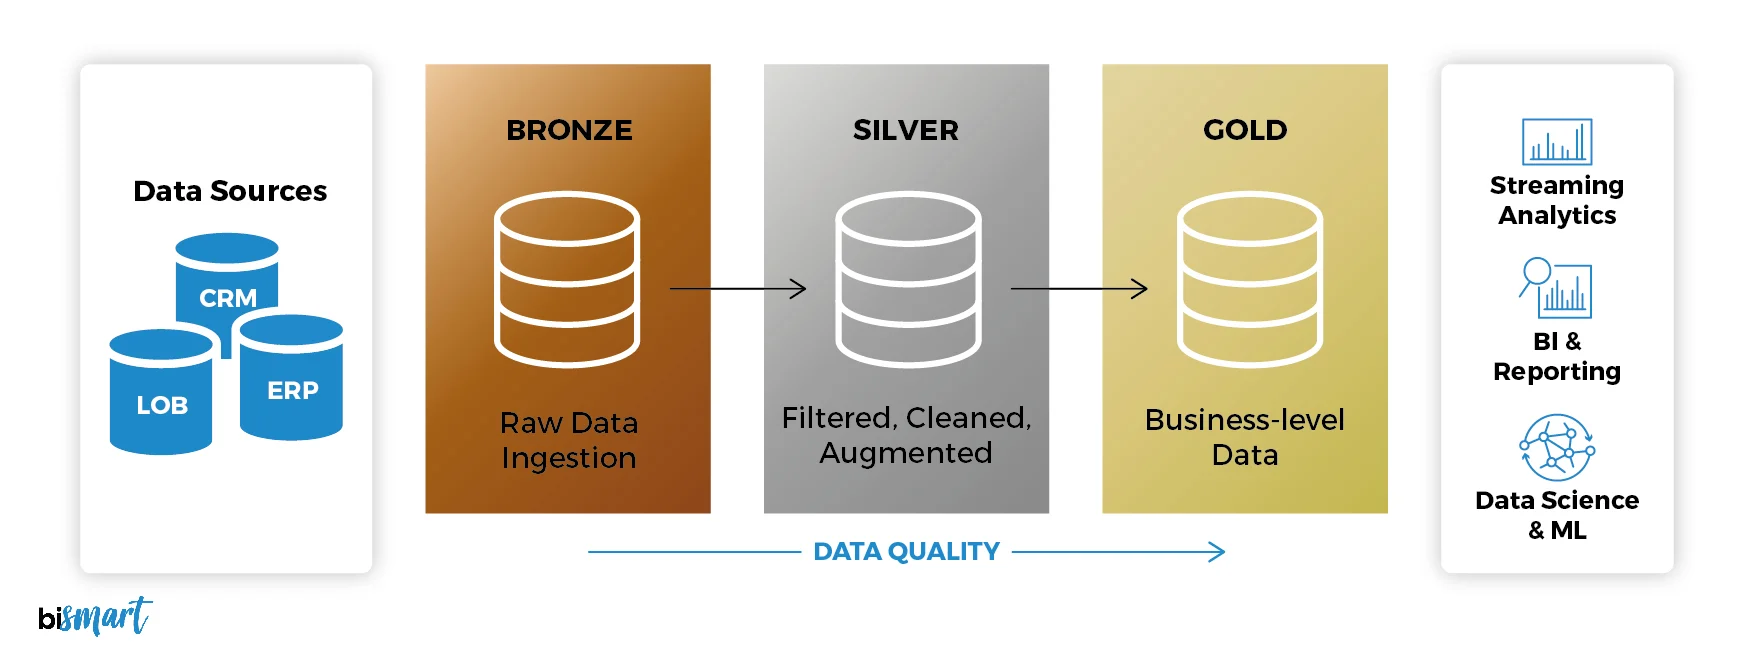
\includegraphics[width=\textwidth]{figures/medallion.png}
    \caption{Medallion architecture for the Lakehouse~\cite{Emilio}.}
    \label{fig:design-decisions-elt-medallion}
\end{figure}

The transformations we plan to implement can be categorized into two types: \ac{sql}-type transformations, which can be fully executed using \ac{sql} statements, and script-type transformations, which require functionality beyond the expressiveness of \ac{sql} (e.g., the functionality of a programming language like Python).
Especially the clean-up transformations between the bronze and silver layers can generally be covered by \ac{sql}-type transformations.

A tool specifically built for efficiently managing \ac{sql}-type transformations for a project is \href{https://www.getdbt.com/}{\textit{dbt}}.
dbt allows us to define \ac{sql} statements in a modular and interconnected manner to ensure data source integrity.
dbt modules are centered around \acp{cte} and feature a dependency mechanism through which different \ac{sql} scripts build on one another.
Additionally, dbt modules can be documented, versioned, tested, and deployed to production.
In this way, dbt serves as the central tool for \ac{sql}-type transformations and becomes more valuable as the number of \ac{sql} statements managed by it increases.

To benefit from the consistently structured handling of \ac{sql} transformations, which we expect to need at least once for each data source between the bronze and silver layers, we choose to adopt dbt early instead of using plain \ac{sql} strings in Python.
The amount of transformations needed between the silver and gold layers is expected to be minimal for now but will likely grow with each additional use case for the available data.


\subsubsection{Workflow Orchestration}
\label{sec:design-decisions-orchestration}

In the previous section, \cref{sec:design-decisions-elt}, we concluded that there are two types of transformations, with only one type covered by dbt.
The script-type transformations are instead to be defined in Python.
Also, our pipeline requires a \ac{gui} to allow for graphical interactions and intuitive insights.

\href{https://dagster.io/}{\textit{Dagster}} is a visual workflow orchestration tool that allows both types of transformations to run, thereby completing our pipeline.
In Dagster, Python functions decorated with \texttt{@asset} appear on the \ac{gui} as workflow elements.
Dagster assets can have dependencies and can therefore form a \ac{dag}, as shown in \cref{fig:design-decisions-orchestration-asset}.

\begin{figure}[H]
    \centering
    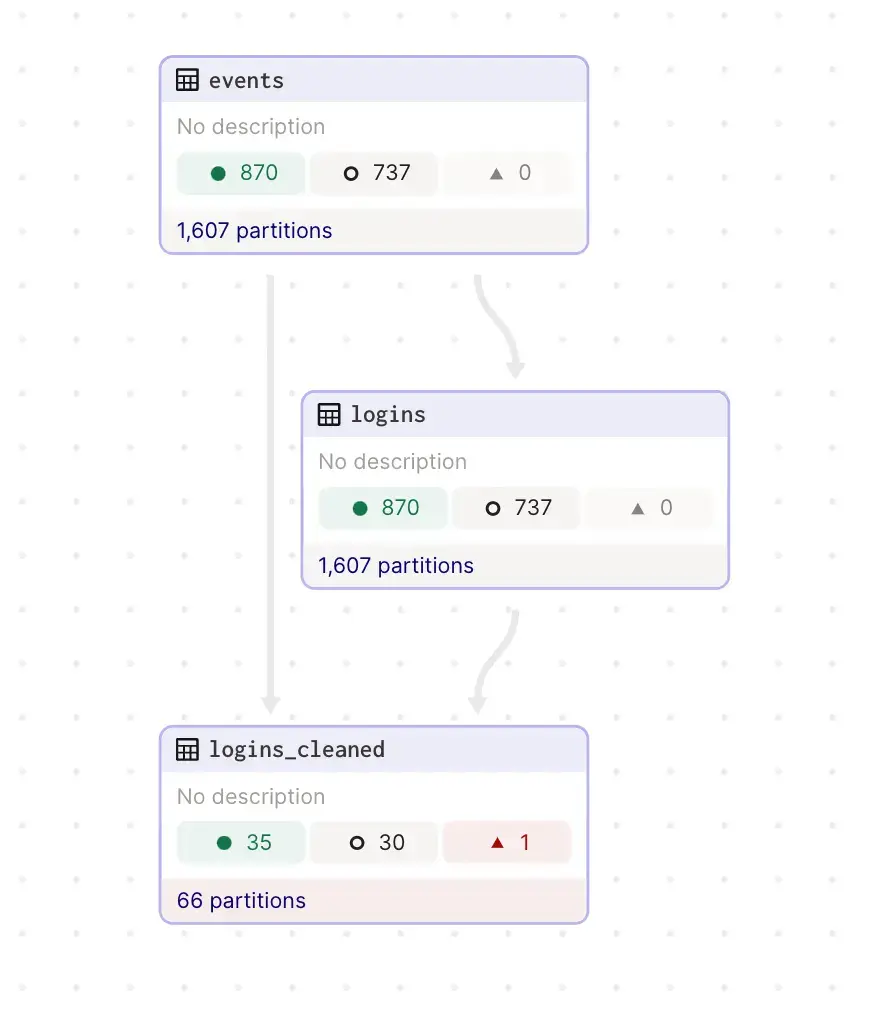
\includegraphics[width=0.6\textwidth]{figures/dagster-partitioned-asset-graph.png}
    \caption{Example of three partitioned Dagster assets forming a \ac{dag}~\cite{Ryza2023}.}
    \label{fig:design-decisions-orchestration-asset}
\end{figure}

With each Dagster asset representing a stored object, such as a table, Dagster offers first-class support for partitioning.
For instance, if hourly partitioning is used, asset runs can be scheduled and backfilled predictably, while maintaining full consistency with parent asset runs.
Alternatively to interval-based asset scheduling, Dagster also allows configuring sensors that trigger asset runs on demand.

Dagster can host multiple workflows sourced from ``code locations'', which can be Python modules or code files.
In development, code changes are loaded without the need to restart Dagster, while in production the Dagster web server can run separately from the user code.

Dagster has a native integration with dbt, mapping dbt's models to Dagster's assets, as shown in \cref{fig:design-decisions-orchestration-dbt}.
A dbt model's filename is interpreted as if it were the name of a Python function with an \texttt{@asset} decorator.
Any references in a dbt model are considered dependencies of a Dagster asset, as specified in the Python function's parameters.

\begin{figure}[H]
    \centering
    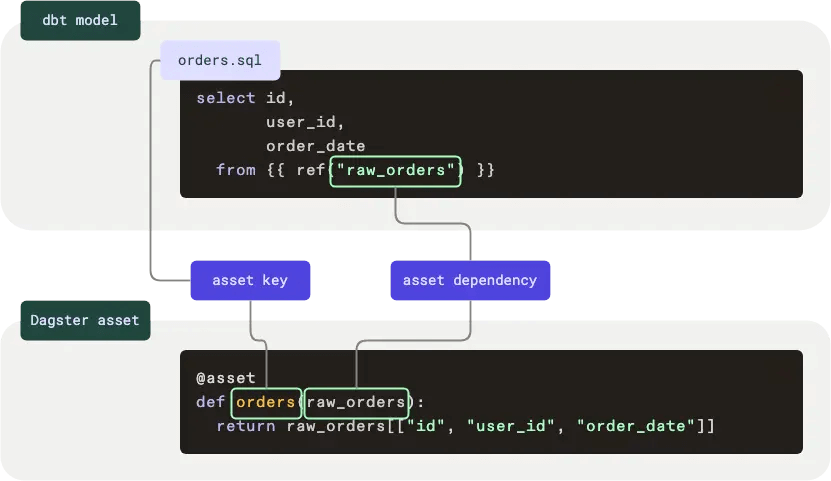
\includegraphics[width=0.8\textwidth]{figures/dagster-dbt.png}
    \caption{Comparison of dbt model and Dagster asset~\cite{DeMaria2022}.}
    \label{fig:design-decisions-orchestration-dbt}
\end{figure}

Alternatives to Dagster include Airflow and NiFi, as introduced in \cref{sec:related-work-big-data-pipelines}.
However, both Airflow and NiFi lack the native partitioning capabilities of Dagster.
Additionally, NiFi is heavily oriented towards real-time processing, emphasizing related quality-of-life features like fine-grained backpressure handling.
In our use case, we do not need to closely track each entity's movement through the system, which saves us some overhead.
Although NiFi pipelines can be configured via low-code \ac{gui} interaction, the available operators for external system interactions, such as those with Iceberg, are limited.
At the time of writing, NiFi only supports adding rows to Iceberg tables, and other interactions like table creation must be done through an external system.

Dagster appears to offer exactly the features we need to orchestrate our pipeline workflow without the limitations of Airflow and NiFi, so we decide to implement Dagster into our pipeline.


\newpage
\acresetall
\cleardoublepage
\section{Implementation}
\label{sec:implementation}

Based on the design defined in \cref{sec:design}, we set up the infrastructure that our pipeline will interact with, using Docker Compose first.
Then, the pipeline itself will be implemented to ingest data, transform it, and output graphs for visualization.
The pipeline's Dockerfile is shown to improve \ac{dx} next, and the resource definitions that enable a production deployment to Kubernetes are provided in the final subsection.

\subsection{Infrastructure}
\label{sec:implementation-infrastructure}

Before implementing the custom code for the pipeline, we first set up the infrastructure components that the pipeline will interact with.
MinIO will be configured for storage and Spark for compute.

The services defined in the following subsections will use various ports.
To maintain an overview of all ports used in the upcoming service definitions, a summary is provided in \cref{sec:appendix-ports}.

\subsubsection{Storage}
\label{sec:implementation-infrastructure-storage}

For \textit{S3} storage, we use MinIO, and for compute, we use Spark with Iceberg support.
The latter is provided by Databricks as a container image.

Two options were evaluated for local multi-container runtimes for development: Kubernetes, to stay as close as possible to the production environment, and \href{https://www.docker.com/}{\textit{Docker}} Compose, due to specific challenges in the local Kubernetes setup.
The challenges faced with setting up Kubernetes locally are described in detail in \cref{sec:appendix-kubernetes}.

Kubernetes, with its advanced architecture and broad feature set, is generally more complex to set up and maintain than Docker Compose, even locally.
Therefore, setting up Kubernetes locally only makes sense if this setup effectively mirrors the production environment.
Otherwise, a simpler solution would be preferable.
In this case, mirroring the production environment involves setting up virtualized block storage with Longhorn, allowing us to test the hypothesis that data will be in reach ``quickly enough'' for efficient computation, as discussed in the storage design section \cref{sec:design-storage}.
Given the challenges referenced above, the alternative container runtime explored next is Docker Compose.

The Docker Compose setup consists mainly of a \texttt{docker-compose.yaml} file and the start/stop commands shown in \cref{lst:docker-compose-commands}\footnote{The \texttt{-d} flag moves execution to the background, freeing the console for additional commands.}.
A tool named \href{https://kompose.io/}{\textit{Kompose}} can later assist in migrating a Docker Compose definition to Kubernetes resource definitions for production deployment, so pivoting to Docker Compose does not entail a significant drawback in this case.

\begin{listing}[H]
\begin{minted}{sh}
docker-compose up (-d)
docker-compose down
\end{minted}
\caption{Docker Compose start and stop commands.}
\label{lst:docker-compose-commands}
\end{listing}

To set up storage with MinIO in Docker Compose, a storage service is defined in \cref{lst:minio-compose}.
We define a named volume, \texttt{minio\_data}, and mount it to the \texttt{/data} directory used by MinIO, ensuring that data persists across Docker Compose restarts.
Automatic restarts upon failure at the service level are desirable, as this aligns with default behaviors in cluster managers like Kubernetes or \href{https://docs.docker.com/engine/swarm/}{\textit{Docker Swarm}}\footnote{Since development sometimes requires stopping a service, such as to avoid hitting rate limits on an external server, it is appropriate to set the service's \texttt{restart} policy to \texttt{unless-stopped}.}.
We expose MinIO's S3 port, 9000, and enable MinIO's web \ac{gui} on port 9001 by modifying MinIO's default start command on line 2.
The image \texttt{minio/minio} is pulled from the \href{https://hub.docker.com/}{\textit{Docker Hub}} registry by default and is versioned with a timestamp format\footnote{A more common versioning scheme used by many other images, including those defined in sections below, is \href{https://semver.org/}{\textit{Semantic Versioning}}.}.

\begin{listing}[H]
\begin{minted}{yaml}
services:
  minio:
    command: ["server", "/data", "--console-address", ":9001"]
    environment:
      MINIO_ROOT_PASSWORD: password
      MINIO_ROOT_USER: admin
    image: minio/minio:RELEASE.2024-10-29T16-01-48Z
    ports:
      - 9000:9000
      - 9001:9001
    restart: unless-stopped
    volumes:
      - minio_data:/data
volumes:
  minio_data: {}
\end{minted}
\caption{Docker Compose definition for MinIO.}
\label{lst:minio-compose}
\end{listing}

For development, MinIO's \ac{gui} is secured by arbitrary credentials set via environment variables, which are replaced by secrets in the production environment.
It is important to note that even in development, hardcoding credentials can pose a security risk, especially in open source projects, as other users on the same network could access services on the developer's machine using the same exposed credentials.

To initialize MinIO with a bucket for storing pipeline data, we define a complementary MinIO client service as shown in \cref{lst:minio-client-compose}.
The \texttt{minio-client} service is set to start only after the \texttt{minio} service has successfully started, specified by the \texttt{depends\_on} relation.
Since the S3 protocol originated from \href{https://aws.amazon.com/}{\textit{\ac{aws}}}, the three environment variables on line 5 are standard for accessing any S3-compatible service, including MinIO in a local setup.

\begin{listing}[H]
\begin{minted}{yaml}
services:
  minio-client:
    depends_on:
      - minio
    environment:
      - AWS_ACCESS_KEY_ID=admin
      - AWS_SECRET_ACCESS_KEY=password
      - AWS_REGION=us-east-1
    entrypoint: >
      /bin/sh -c "
      until (/usr/bin/mc config host add minio http://minio:9000 admin password) do echo '...waiting...' && sleep 1; done;
      /usr/bin/mc mb minio/lakehouse;
      /usr/bin/mc anonymous set public minio/lakehouse;
      tail -f /dev/null
      "
    image: minio/mc:RELEASE.2024-10-29T15-34-59Z
    restart: unless-stopped
\end{minted}
\caption{Docker Compose definition for MinIO's client.}
\label{lst:minio-client-compose}
\end{listing}

The \texttt{entrypoint} defines a script that waits until the MinIO service is reachable via \ac{http}, then creates a bucket named \texttt{lakehouse}, makes it publicly accessible, and runs a persistent command to prevent the container from restarting.
An alternative would be to modify the \texttt{restart} property to avoid restarting on success, but we aim to stay as close as possible to typical container cluster behavior.
In Kubernetes, this service would be implemented as a \textit{Job} that restarts on failure but not on success, a feature unavailable in Docker Compose.
To work around this limitation, the final \texttt{tail -f /dev/null} command ensures the container remains running.

With the definitions for the MinIO and MinIO client services, our simple and standardized storage setup is complete.

\subsubsection{Compute}
\label{sec:implementation-infrastructure-compute}

Next, we set up Spark as the computation engine in Docker Compose.
Since Spark is intended to read from and write to Iceberg tables, Iceberg support must be added to Spark.
Additionally, it is beneficial to have a \ac{gui} during development for testing Spark commands with Iceberg support.
These requirements are fulfilled by the \texttt{spark-iceberg} container image provided by \textit{Tabular}\footnote{The backing repository was migrated to \href{https://github.com/databricks/}{Databricks' GitHub organization} during the course of this thesis.}, which we use instead of the \href{https://docs.docker.com/trusted-content/official-images/}{\textit{Docker Official Images}} \texttt{spark} image, as the latter lacks these additions.

However, the \texttt{spark-iceberg} image's latest release dates back eight months, likely due to Databricks' acquisition of the former maintaining company, Tabular~\cite{Databricks2024}.
Because Iceberg is currently under active development, using a recent Iceberg version minimizes the chance of encountering bugs.
We therefore use a custom fork of the \texttt{spark-iceberg} image, available on the \ac{ghcr}, which includes Spark \texttt{3.5.3} and Iceberg version \texttt{1.6.1}.

\begin{listing}[H]
\begin{minted}{yaml}
services:
  spark-iceberg:
    image: ghcr.io/dargmuesli/spark-iceberg:3.5.3_1.6.1
    depends_on:
      - rest
      - minio
    environment:
      - AWS_ACCESS_KEY_ID=admin
      - AWS_SECRET_ACCESS_KEY=password
      - AWS_REGION=us-east-1
    ports:
      - 7077:7077
      - 8888:8888
      - 8080:8080
      - 10000:10000
    restart: unless-stopped
    volumes:
      - ./docker/spark/entrypoint-master.sh:/opt/spark/entrypoint.sh
      - ./docker/spark/spark-defaults.conf:/opt/spark/conf/spark-defaults.conf
\end{minted}
\caption{Docker Compose definition for Spark's master.}
\label{lst:compose-spark-master}
\end{listing}

\Cref{lst:compose-spark-master} shows the Spark image running as the Spark master service.
A volume overrides Spark's default settings file, \texttt{spark-defaults.conf}, as specified on line 19, with options shown in \cref{lst:spark-defaults}, particularly to configure Spark to use a \ac{rest} catalog backed by S3 for unified storage.
The image's default entrypoint is also overridden on line 19 with a script detailed in \cref{lst:spark-master-entrypoint} that performs the following:

\begin{enumerate}
    \item Binds the Spark master to port 7077.
    \item Starts an \href{https://thrift.apache.org/}{\textit{Apache Thrift}} server on port 10000, enabling \acp{rpc} through various programming languages\footnote{The Thrift connection will be used by dbt later.}.
    \item Creates Iceberg table namespaces, notably the \texttt{default} namespace\footnote{dbt requires the \texttt{default} namespace to connect successfully.}.
\end{enumerate}

Port 8888 is used for the Spark master \ac{gui}, and port 8080 for the Jupyter Notebook \ac{gui}.
As specified on line 5, the service expects a \texttt{rest} service as a catalog interface, defined in \cref{lst:compose-rest}.

\begin{listing}[H]
\begin{minted}{yaml}
services:
  rest:
    environment:
      - AWS_ACCESS_KEY_ID=admin
      - AWS_SECRET_ACCESS_KEY=password
      - AWS_REGION=us-east-1
      - CATALOG_IO__IMPL=org.apache.iceberg.aws.s3.S3FileIO
      - CATALOG_S3_ENDPOINT=http://minio:9000
      - CATALOG_S3_PATH__STYLE__ACCESS=true
      - CATALOG_WAREHOUSE=s3://lakehouse/
    image: ghcr.io/dargmuesli/iceberg-rest:1.6.1
    ports:
      - 8181:8181
    restart: unless-stopped
\end{minted}
\caption{Docker Compose definition for Spark's \ac{rest} catalog wrapper.}
\label{lst:compose-rest}
\end{listing}

Similarly to the previously described image \texttt{spark-iceberg}, the \texttt{rest} service also uses a fork of a Tabular image called \texttt{iceberg-rest}.
It is essential to ensure that all services are configured with the same tool versions to prevent compatibility errors.
The \texttt{rest} service exposes port 8181, is configured to use MinIO as the S3 storage backend, and, importantly, is set to use S3's path-style access.

By default, the \texttt{org.apache.iceberg.aws.s3} package properties enable a \textit{Virtual Host} style for bucket access.
With Virtual Host style, buckets are accessible as subdomain-like hostnames, e.g., \texttt{http://lakehouse.minio}, where \texttt{lakehouse} is the bucket name and \texttt{minio} is the service hostname, routable in the Docker Compose default network.
In contrast, the path style makes the \texttt{lakehouse} bucket accessible at \texttt{http://minio/lakehouse}.
Docker Compose can set network aliases for services, allowing MinIO to be configured for Virtual Host-style access through the incremental configuration shown in \cref{lst:compose-mino-virtual-host}.
However, setting up Virtual Host-style access in Kubernetes is more complex due to hostname syntax limitations involving dot characters.
Therefore, the \texttt{rest} service is configured to use path-style access instead.

Finally, Spark is intended to compute in a distributed manner, requiring the addition of worker services.
Even in development, adding worker services is beneficial for verifying inter-service communication.
\Cref{lst:compose-spark-worker} shows the Docker Compose service definition for Spark workers with deployment replicas scaled to two.

\begin{listing}[H]
\begin{minted}{yaml}
services:
  spark-iceberg-worker:
    deploy:
      replicas: 2
    image: ghcr.io/dargmuesli/spark-iceberg:3.5.3_1.6.1
    depends_on:
      - spark-iceberg
    environment:
      - AWS_ACCESS_KEY_ID=admin
      - AWS_SECRET_ACCESS_KEY=password
      - AWS_REGION=us-east-1
    restart: unless-stopped
    volumes:
      - ./docker/spark/entrypoint-worker.sh:/opt/spark/entrypoint.sh
      - ./docker/spark/spark-defaults.conf:/opt/spark/conf/spark-defaults.conf
\end{minted}
\caption{Docker Compose definition for a Spark worker.}
\label{lst:compose-spark-worker}
\end{listing}

The workers use the same image as the master.
The primary distinction between the worker and the master is the entrypoint script being mounted.
The worker entrypoint script, detailed in \cref{lst:spark-worker-entrypoint}, performs the following actions:

\begin{enumerate}
    \item Installs necessary dependencies for script execution\footnote{The design of dependency installation in worker containers is evaluated in \cref{sec:evaluation-objectives}.}.
    \item Binds the worker to port 8787 and configures it to connect to the Spark master.
\end{enumerate}

Additionally, the workers do not expose any ports, as they establish a connection with the master.
This setup allows the master to dynamically connect with any number of workers without needing to know their exact identities, thus supporting scalability.
With this, the setup of Spark as the compute engine is complete.

\subsection{Pipeline}
\label{sec:implementation-pipeline}

This section describes the custom pipeline implementation using the tools selected in \cref{sec:design-decisions-elt}.
To support flexible data ingestion, we initialize a Python project using the dependency manager \href{https://python-poetry.org/}{\textit{Poetry}}.

Since Spark is built with Python version \texttt{3.11}, we constrain our project to this version for optimal compatibility.
We add a \texttt{.python-version} file containing \texttt{3.11} and specify \texttt{python = ">=3.11,<3.12"} as the version range in Poetry's \texttt{pyproject.toml}.
We also include the following primary dependencies:

\begin{itemize}
    \item \textbf{dagster} for task orchestration,
    \item \textbf{dagster-dbt} for integrating dbt resources with Dagster, and
    \item \textbf{pyspark} for Spark computations.
\end{itemize}

Additional dependencies used in the custom pipeline code include:

\begin{itemize}
    \item \textbf{fastwarc} for parsing Common Crawl's \ac{warc} files,
    \item \textbf{iso3166} for country ID transformations,
    \item \textbf{lxml}, an optional addition to enable Pandas to fetch tables from remote \ac{html},
    \item \textbf{pandas} for converting Pandas DataFrames to and from Spark DataFrames,
    \item \textbf{plotly} as a visualization library for generating graphs,
    \item \textbf{pympler}, a helper for retrieving the full size of nested objects, and
    \item \textbf{tenacity} for implementing exponential backoff retries for web requests used in data ingestion.
\end{itemize}

Finally, the following dependencies are required for building the production image:

\begin{itemize}
    \item \textbf{dagster-webserver}, a subcomponent of \texttt{dagster} alongside \texttt{dagster-daemon}, responsible for schedules, sensors, and run queueing,
    \item \textbf{dbt-spark} with the \texttt{pyhive} extra, enabling dbt project builds even when constructing the Dagster project.
\end{itemize}


\subsubsection{Ingestion}
\label{sec:implementation-pipeline-ingestion}

The first source for ingestion is the Common Crawl dataset.
We create a Dagster asset, as shown in \cref{lst:dagster-source-common-crawl}, to iterate over \ac{warc} files and write batches of extracted content to our storage.
A Dagster asset is comparable to a task in AirFlow and appears as an element within the task graph in Dagster's \ac{gui}.
This and subsequent listings are simplified variants of the actual source code, optimized for readability and brevity.

\begin{listing}[H]
\begin{minted}{python}
class Configuration(Config):
  dataset_id: str | None
  dataset_subset: str = "warc"
  path_filter_regex: str | None
  max_batch_size: int = 1073741824 # bytes = 1 GiB

@asset(kinds={"python", "spark"})
async def source_common_crawl(configuration: Configuration):
  """Ingests Common Crawl's WARC files."""
  warcs = fetch_warc_records(
    configuration.dataset_id,
    configuration.dataset_subset,
    configuration.path_filter_regex
  )

  for warc in warcs:
    warc_batched = batch_records(
      warc,
      configuration.max_batch_size
    )
    await process_batch(
      warc_batched,
      write_source
    )
\end{minted}
\caption{Dagster asset for Common Crawl ingestion.}
\label{lst:dagster-source-common-crawl}
\end{listing}

The asset is visualized on the Dagster dashboard as shown in \cref{fig:dagster-source-common-crawl-source}.
The function name (line 8) is defined first, followed by the function's description (line 9).
The tag ``Never materialized'' indicates that the workflow item has not yet been executed, while the \texttt{python} and \texttt{spark} tags below denote the technologies specified on line 7 of \cref{lst:dagster-source-common-crawl}.
These tags align with Dagster's \texttt{dbt} integration outlined in \cref{sec:implementation-pipeline-transformation}, which similarly tags its assets, ensuring consistent visuals across all assets.

\begin{figure}[H]
  \centering
  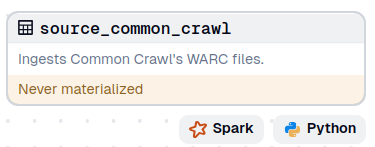
\includegraphics[width=0.4\textwidth]{figures/dagster-common-crawl-source.png}
  \caption{Common Crawl ingestion asset on Dagster's dashboard.}
  \label{fig:dagster-source-common-crawl-source}
\end{figure}

At the top of \cref{lst:dagster-source-common-crawl}, a \texttt{Configuration} class defines parameters passed to the asset, allowing for the following customizations:

\begin{itemize}
    \item \textbf{dataset\_id} allows specification of a Common Crawl dataset, with the default set to the most recent dataset.
        For instance, setting \texttt{CC-MAIN-2024-42} accesses data from October 2024, while \texttt{CC-MAIN-2024-33} refers to August 2024.
        This flexibility is crucial, as each dataset contains approximately 100~TiB of compressed data, requiring significant ingestion time, especially since new datasets are released monthly.
    \item \textbf{dataset\_subset} enables users to ingest data beyond the default \ac{warc} files, which contain only responses with status code \texttt{200}.
        For example, setting \texttt{non200responses} allows ingestion of \ac{http} responses with status codes indicating unsuccessful results—a dataset comprising around 2.5~TiB of compressed data across 90,000 files in Common Crawl.
    \item \textbf{path\_filter\_regex} specifies which of the approximately 90,000 \ac{warc} files to load from a dataset.
        For example, the regex \texttt{\textasciicircum.+-00000\textbackslash.warc\textbackslash.gz\$} restricts processing to 100 files, selecting one file per batch of 900 \ac{warc} files.
        By default, only the first \ac{warc} file is processed; a regex like \texttt{*} can be used for full dataset ingestion in production.
    \item \textbf{max\_batch\_size} adjusts the data size in each Spark job.
        While Spark jobs default to 128 MiB, we configure Spark to handle jobs up to 1 GiB to improve performance, aligning with this parameter's default.
        This setting primarily provides flexibility if smaller job sizes prove necessary.
\end{itemize}

\Cref{lst:dagster-source-common-crawl-fetch} demonstrates how Common Crawl data is fetched via its secure \ac{http} \ac{api}.
First, the available datasets are pulled from Common Crawl's index (lines 3 and 4) if no \texttt{dataset\_id} is specified.
Next, \ac{warc} file metadata for the given dataset is pulled from Common Crawl's data storage, as shown in lines 16 to 20.
The metadata is compressed with \href{https://www.gnu.org/software/gzip/}{\textit{gzip}} and must be decompressed (line 24) and decoded in \href{https://www.unicode.org/versions/latest/}{\texttt{UTF-8}} (line 25).
Finally, each \ac{warc} file is fetched in the last function, defined from lines 40 to 45.
Two Python decorators serve as helper functions in \cref{lst:dagster-source-common-crawl-fetch}:

\begin{itemize}
    \item \textbf{measure\_performance} is a custom function that helps identify performance bottlenecks by using Python's built-in time and logging functionalities, as specified in \cref{lst:dagster-utility-performance-measurement}.
    \item \textbf{retry} is the exponential backoff implementation from the \texttt{tenacity} library, enabling retries on temporary \ac{http} 503 error responses.
\end{itemize}

The main ingestion logic is outlined in \cref{lst:dagster-source-common-crawl-warc}.
The archive stream retrieved from the previously fetched \ac{warc} files via the \texttt{fastwarc} library is passed in at line 3, along with the dataset ID on line 4.
For each record within the stream, validations are performed for parsing success, content type, record type, \ac{http} status code, charset, and \ac{uri} validity.
These validations are represented by comments in the listing for brevity.
If the record passes these checks, the \ac{html} response within the record is decoded (line 19), and the sizes for both the encoded and decoded versions are measured (lines 23 and 24).
Finally, records that meet the table schema requirements are yielded\footnote{Values yielded by this function can be iterated over by calling functions. The function in \cref{lst:dagster-source-common-crawl-warc} is a Python \href{https://wiki.python.org/moin/Generators}{\textit{Generator}}.} (lines 26 to 34).

\begin{listing}[H]
\begin{minted}{python}
@measure_performance
def get_warc_records(
    records: ArchiveIterator,
    dataset_id: str
):
    for record in records:
        # ...http parsing verification...

        if record.http_content_type != "text/html":
            continue # skip non-html content like PDFs or XML files

        # ...record type, status code, charset and target uri verification...

        response_target_uri = record.headers.get("WARC-Target-URI")
        response_charset = record.http_charset
        response_payload = record.reader.read()

        try:
            response_payload_decoded = response_payload.decode(response_charset or "utf-8")
        except UnicodeDecodeError:
            # ...retry logic...

        response_payload_size_bytes = len(response_payload)
        response_payload_decoded_length = len(response_payload_decoded)

        yield {
            "dataset_id": dataset_id,
            "response_charset": response_charset,
            "response_headers_status_code": record.http_headers.status_code,
            "response_payload": response_payload_decoded,
            "response_payload_size_bytes": response_payload_size_bytes,
            "response_payload_length": response_payload_decoded_length,
            "response_target_uri": response_target_uri,
        }
\end{minted}
\caption{Extraction of Common Crawl's \ac{warc} data.}
\label{lst:dagster-source-common-crawl-warc}
\end{listing}

The records extracted from the \ac{warc} files are then accumulated until a specific batch size is reached by the function defined in \cref{lst:dagster-utility-performance-batching}.
To further enhance performance, a queue of such batches is used, allowing multiple batches to be generated in advance while they are sequentially processed in the next step.
The queuing mechanism improves performance by ensuring the immediate availability of the next item for processing.
If each batch were generated only after the preceding batch completed its processing, valuable time would be lost in generating the next item.
This queue implementation leverages Python's asynchronous \ac{io} module, as shown in \cref{lst:dagster-utility-performance-queuing}.

To complete the ingestion tooling, we configure a Spark client for writing extracted records to Iceberg tables.
\Cref{lst:dagster-utility-spark} shows a PySpark client instance, named \texttt{SparkSession}, implemented with a \textit{Singleton} pattern.
The Spark driver is configured to receive inbound traffic on port 7777, which would otherwise be randomly selected.
Specifying a port allows us to establish strict networking rules in Kubernetes, though this is unnecessary when running in Docker Compose.
Similarly, port 7878 is set for Spark's block manager, which supports data broadcasting to executors.
Most other configuration settings align with those previously discussed for Spark configurations, such as the \texttt{rest} service setup in \cref{sec:implementation-infrastructure-compute}.

The Spark client configuration also provides flexible memory reservation for the Spark driver and executors: 50~G is reserved when running on a Kubernetes cluster and 4~G when running in Docker Compose.
In this context, running on Kubernetes equates to production, and these memory values (50~G and 4~G) are chosen based on the available memory on the production and development machines.

To complete the Common Crawl ingestion, the fetched data is written to its designated Iceberg table.
\Cref{lst:dagster-source-common-crawl-write} shows a general, type-safe approach for writing to this table.
The schema defined in the initial lines ensures that a table can be created even when the initial data does not clearly allow for schema inference -- for example, when a column filled exclusively with \texttt{null} values makes it impossible to determine an appropriate type such as \texttt{string} or \texttt{integer}.

The logic for choosing between appending to or creating a table (lines 15 to 18) could be streamlined if a \texttt{createOrAppend} command were available.
Although a \texttt{MERGE INTO} \ac{sql} command exists for Iceberg, it is only accessible via the \textit{Data Source V2} \ac{api} in Spark \texttt{4}, which has not yet been released at the time of writing~\cite{Gao2023}.
The \texttt{spark\_dataframe.mergeInto("table")} function in Spark \texttt{4} would also prevent duplicate row insertions, which are currently managed manually, as shown in \cref{lst:dagster-source-common-crawl-write-deduplicated}.
\Cref{fig:analysis-pipeline-performance-driver} shows the Spark driver's query diagram for this data appending operation.
Tables with few rows, where full refreshes are feasible with each update, may alternatively use \texttt{spark\_dataframe.createOrReplace("table")}.

\begin{listing}[H]
\begin{minted}{python}
SCHEMA = StructType(
  [
    StructField("dataset_id", StringType(), False),
    StructField("response_headers_status_code", IntegerType(), False),
    # ...more fields...
  ]
)
TABLE = "raw.source_common_crawl"


def write_source(batch: list):
  is_table_existing = SparkManager.spark.catalog.tableExists(TABLE)
  dataframe = SparkManager.spark.createDataFrame(batch, SCHEMA)

  if is_table_existing:
    dataframe.writeTo(TABLE).append()
  else:
    dataframe.writeTo(TABLE).partitionedBy("dataset_id", "response_charset").create()
\end{minted}
\caption{Writing entries to a partitioned Iceberg table.}
\label{lst:dagster-source-common-crawl-write}
\end{listing}

We have now defined a complete ingestion flow into the bronze layer, as defined in \cref{sec:design-decisions-elt}.
Next, we proceed with transformations from the bronze layer to the silver and gold layers.


\subsubsection{Transformation}
\label{sec:implementation-pipeline-transformation}

With data ingested into the bronze layer, represented by the namespace \texttt{raw}, we first use dbt to transform data into the silver layer, represented by the namespace \texttt{staging}.
We then use a Dagster Python asset to combine all silver-layer tables into a \texttt{fact} table stored in the gold layer.

Python is used instead of dbt for the final transformation to showcase how a transformation leveraging a third-party Python module can be implemented, extending beyond the capabilities of \ac{sql} statements.
This Python example also illustrates the potential for bidirectional asset connections in Dagster, meaning connections can be made from Python assets to dbt models and vice-versa.

Given the distinct natures of our two transformation types, dbt code is primarily declarative, while Python code is imperative.
The following code listings will therefore primarily show configuration declarations instead of imperative code for dbt.

A basic dbt setup includes a project configuration and a profile configuration.
The project configuration allows us to define models, seeds, snapshots, variables, and general project settings, such as name and version, as well as adjust the directory paths where dbt expects to find source files.
The profile configuration defines storage connections.

Similar to \cref{sec:implementation-pipeline}, we set up a new dbt project named \texttt{transformation} with the following dependencies managed by Poetry:

\begin{itemize}
  \item \textbf{dbt-core} for dbt itself.
  \item \textbf{dbt-spark} with the \texttt{PyHive} extra to enable dbt connections to Spark via Thrift.
\end{itemize}

Our dbt project configuration, shown in \cref{lst:implementation-pipeline-transformation-dbt-project}, sets \texttt{iceberg} as the file format on lines 5 and 11 and outputs to the \texttt{staging} namespace\footnote{In dbt, a schema is equivalent to an Iceberg database and namespace.} (line 9), materialized as a view (line 8).
The straightforward transformations we perform, such as renaming columns and excluding rows where certain fields are \texttt{null}, do not require table materialization, which would largely result in duplicated data.
An additional option dbt offers is incremental materialization, which only processes new and updated data based on a specified strategy, such as \texttt{append} or \texttt{merge}.
For our basic transformations, a view is both sufficient and efficient.

Our dbt project is also configured with a seed table named \texttt{seed\_common\_crawl} in the \texttt{raw} namespace (starting from line 10).
With the configuration in \cref{lst:implementation-pipeline-transformation-dbt-project}, dbt loads a \ac{csv} file named \texttt{seed\_common\_crawl} into an identically named table within the \texttt{raw} namespace when running \texttt{dbt seed}.

\begin{listing}[H]
\begin{minted}{yaml}
name: 'transformation'
profile: 'transformation'
# ...more properties...
models:
  +file_format: iceberg
  transformation:
    staging:
      +materialized: view
      +schema: staging
seeds:
  +file_format: iceberg
  +schema: raw
  transformation:
    seed_common_crawl:
      +column_types:
        dataset_id: string
        response_headers_status_code: int
        # ...more columns...
\end{minted}
\caption{Configuration of our dbt project.}
\label{lst:implementation-pipeline-transformation-dbt-project}
\end{listing}

\Cref{lst:implementation-pipeline-transformation-dbt-model} shows the definition for the dbt model \texttt{dimension\_web\_technologies}.
This model is configured to select four columns (lines 1 to 5) from the bronze layer's \texttt{raw.source\_common\_crawl} table, renaming one of the columns (line 3) and ensuring all rows have values in two columns (line 6).
Line 6 includes a templating expression that is not part of the \ac{sql} standard; dbt replaces this with the appropriate value using Python's \href{https://jinja.palletsprojects.com/}{Jinja} templating engine.
To use a seed instead of a table as a source, one could specify \texttt{ref('seed\_web\_technologies')} on line 6.

\begin{listing}[H]
\begin{minted}{sql}
SELECT
  description,
  html AS html_regular_expressions,
  name,
  website
FROM {{ source('raw', 'source_web_technologies') }}
WHERE html IS NOT NULL AND name IS NOT NULL
\end{minted}
\caption{The dbt model \texttt{dimension\_web\_technologies}.}
\label{lst:implementation-pipeline-transformation-dbt-model}
\end{listing}

In addition to a model definition, we also define a dbt macro, shown in \cref{lst:implementation-pipeline-transformation-dbt-macro}, to demonstrate dbt's testing capabilities.
Beyond built-in checks like \texttt{not\_null} and \texttt{unique}, this custom check validates that only expected status codes have been transformed into the silver stage.
If the query in the macro returns any values, the transformation fails, printing the number of offending rows.

\begin{listing}[H]
\begin{minted}{sql}

SELECT *
FROM {{ model }}
WHERE ({{ column_name }} < 200 OR {{ column_name }} > 599)

\end{minted}
\caption{A dbt macro that checks for a reasonable \ac{http} status code.}
\label{lst:implementation-pipeline-transformation-dbt-macro}
\end{listing}

\Cref{lst:implementation-pipeline-transformation-dbt-models} now integrates all components by referencing models and sources, thus making them visible to dbt.
First, the model \texttt{dimension\_common\_crawl} defined in \cref{lst:implementation-pipeline-transformation-dbt-model} is declared.
The macro from \cref{lst:implementation-pipeline-transformation-dbt-macro} is applied as a test on the column \texttt{response\_headers\_status\_code} (line 9), alongside a \texttt{not\_null} test.

Line 5 sets a description for the column using the templating syntax familiar from the macro definition.
An example documentation definition is provided in \cref{lst:appendix-listings-dbt-doc}.
The full project documentation can be generated and served using the commands specified in \cref{lst:implementation-pipeline-transformation-dbt-docs}.
An example screenshot of dbt's comprehensive project documentation is shown in \cref{fig:appendix-guis-dbt-docs}.

To make the \texttt{raw} namespace available as a source, it is declared starting on line 12.
It is important to note that lines 19 to 21 define an asset key as metadata, which allows Dagster to link dbt models to their dependencies.
Additionally, dbt enables freshness checks on source data, as shown from line 22 onward.

\begin{listing}[H]
\begin{minted}{yaml}
models:
  - name: dimension_common_crawl
    columns:
      - name: response_headers_status_code
        description: '{{ doc("common_crawl__response_headers_status_code") }}'
        data_type: number
        data_tests:
          - not_null
          - is_between_200_and_599
    #...more columns...
  #...more models...
sources:
  - name: raw
    tables:
      - name: source_common_crawl
        columns:
          - name: response_headers_status_code
          #...more columns...
        meta:
          dagster:
            asset_key: ["source_common_crawl"]
    freshness:
      warn_after: {count: 150, period: day}
      error_after: {count: 365, period: day}
      filter: datediff('year', dataset_year, current_timestamp) < 2
    loaded_at_field: dataset_year
  #...more sources...
\end{minted}
\caption{Definition of dbt models and sources.}
\label{lst:implementation-pipeline-transformation-dbt-models}
\end{listing}

Having explored the dbt project configuration and model definitions in detail, we now move back to the root-level profile definitions, which then lead us toward Dagster.
The profiles shown in \cref{lst:implementation-pipeline-transformation-dbt-profiles} allow dbt commands executed via the command line to use a different host than when run inside a container.
Line 15 specifies the default profile, \texttt{cli}, which is used by the command line if not overridden by the respective command-line argument.

\begin{listing}[H]
\begin{minted}{yaml}
transformation:
  outputs:
    cli:
      type: spark
      method: thrift
      schema: default
      host: 127.0.0.1
      port: 10000
    internal:
      type: spark
      method: thrift
      schema: default
      host: spark-iceberg
      port: 10000
  target: cli
\end{minted}
\caption{Configuration of dbt profiles.}
\label{lst:implementation-pipeline-transformation-dbt-profiles}
\end{listing}

Dagster integrates dbt as shown in \cref{lst:implementation-pipeline-transformation-dagster-dbt}, where line 9 specifies the use of the \texttt{internal} profile instead of the default \texttt{cli} profile for \acp{rpc} initiated by Dagster.
Line 2 locates the dbt project in a directory named \texttt{transformation}.
Line 19 commands the dbt project to be built, generating a dbt manifest file that Dagster uses to learn about the dbt project's models and seeds.

\begin{listing}[H]
\begin{minted}{python}
project = DbtProject(
  project_dir=Path(__file__).joinpath("transformation").resolve(),
)

Definitions(
  resources={
    "dbt": DbtCliResource(
      project_dir=project,
      target="internal"
    ),
  },
)

@dbt_assets(manifest=project.manifest_path)
def transformation_dbt_assets(
  context: AssetExecutionContext,
  dbt: DbtCliResource,
):
  yield from dbt.cli(["build"], context=context).stream()
\end{minted}
\caption{Integration of the dbt project into Dagster.}
\label{lst:implementation-pipeline-transformation-dagster-dbt}
\end{listing}

Our dbt project is now fully integrated with Dagster and the Dagster \ac{gui} displays it as shown in \cref{fig:dagster-source-common-crawl}.
There are two new boxes with dbt tags, representing the seed declared in \cref{lst:implementation-pipeline-transformation-dbt-project} and the model definition from \cref{lst:implementation-pipeline-transformation-dbt-model}.
The silver layer's dimension asset also lists seven checks, representing the total number of tests like \texttt{is\_between\_200\_and\_599} or \texttt{not\_null} across all columns.
A gray dot is shown next to the number seven, indicating that none of the tests have been executed yet.

\begin{figure}[H]
  \centering
  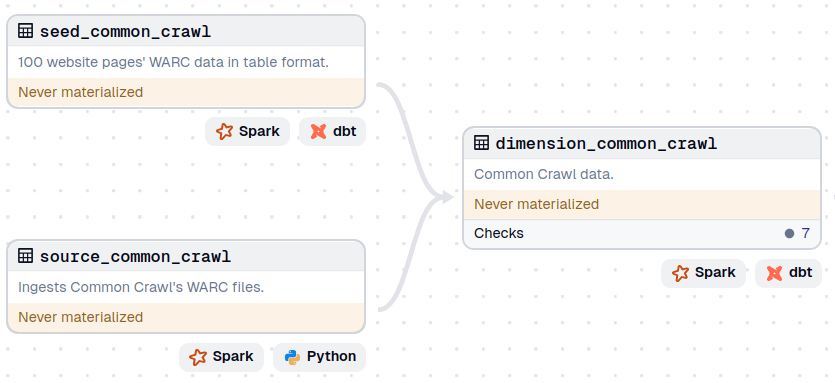
\includegraphics[width=0.75\textwidth]{figures/dagster-common-crawl.png}
  \caption{Common Crawl bronze and silver layers' assets on Dagster's dashboard.}
  \label{fig:dagster-source-common-crawl}
\end{figure}

The only remaining transformation is between the silver layer and the gold layer.
As this is a more complex transformation\footnote{Another similar transformation, not shown here for brevity, uses a third-party Python library.}, we use Python instead of dbt, as shown in \cref{lst:implementation-pipeline-transformation-fact}.

Lines 1 to 8 define a Dagster asset that depends on the dbt model \texttt{dimension\_common\_crawl}.
The complex transformation is defined as a lambda function in lines 13 to 20.
The function takes in \ac{html} code, searches for web technology usage within the \ac{html} code via \ac{regex} pattern matching, and returns a list of detected web technology names.
To use this function with Spark, it is converted into a \ac{udf} in lines 21 to 24.
The \ac{udf} is then applied to a column containing \ac{html} data (line 28), creating a new \texttt{web\_technologies} column in the existing DataFrame.
The final result is written to the \texttt{fact\_website} table in the \texttt{marts} namespace, representing the gold layer.

\begin{listing}[H]
\begin{minted}{python}
@asset(
  deps=[
      get_asset_key_for_model(
        [transformation_dbt_assets], "dimension_common_crawl"
      ),
  ],
  kinds={"python", "spark"},
)
def fact_website():
  web_technologies = SparkManager.spark.table(
    "staging.dimension_web_technologies"
  ).collect()
  get_web_technologies: Callable[[str], list[str]] = lambda html: [
      web_technology["name"]
      for web_technology in web_technologies
      if any(
          re.search(regular_expression, html)
          for regular_expression in web_technology["html_regular_expressions"]
      )
  ]
  get_udf = udf(
    get_web_technologies,
    ArrayType(StringType())
  )

  common_crawl = SparkManager.spark.table("staging.dimension_common_crawl")
  common_crawl = common_crawl.withColumn(
      "web_technologies", get_udf(common_crawl["response_payload"])
  )
  common_crawl.writeTo("marts.fact_website").createOrReplace()
\end{minted}
\caption{Transformation of staging tables into a fact table.}
\label{lst:implementation-pipeline-transformation-fact}
\end{listing}

The result, along with two additional source definitions for country codes and web technologies (omitted here for brevity), is displayed in \cref{fig:implementation-dx-dashboard}.
In that figure, parts of the overall workflow have been executed or are currently running.
All assets in the bronze layer and one dimension table have been successfully materialized.
The \texttt{dimension\_common\_crawl} asset was materialized, with one check having failed, one succeeded, and five still in progress.
The \texttt{dimension\_web\_technologies} asset shows all checks failing, indicating an issue with the dependent source table.
The gold layer's \texttt{fact\_table} asset is still in the process of materializing.

\begin{figure}[H]
  \centering
  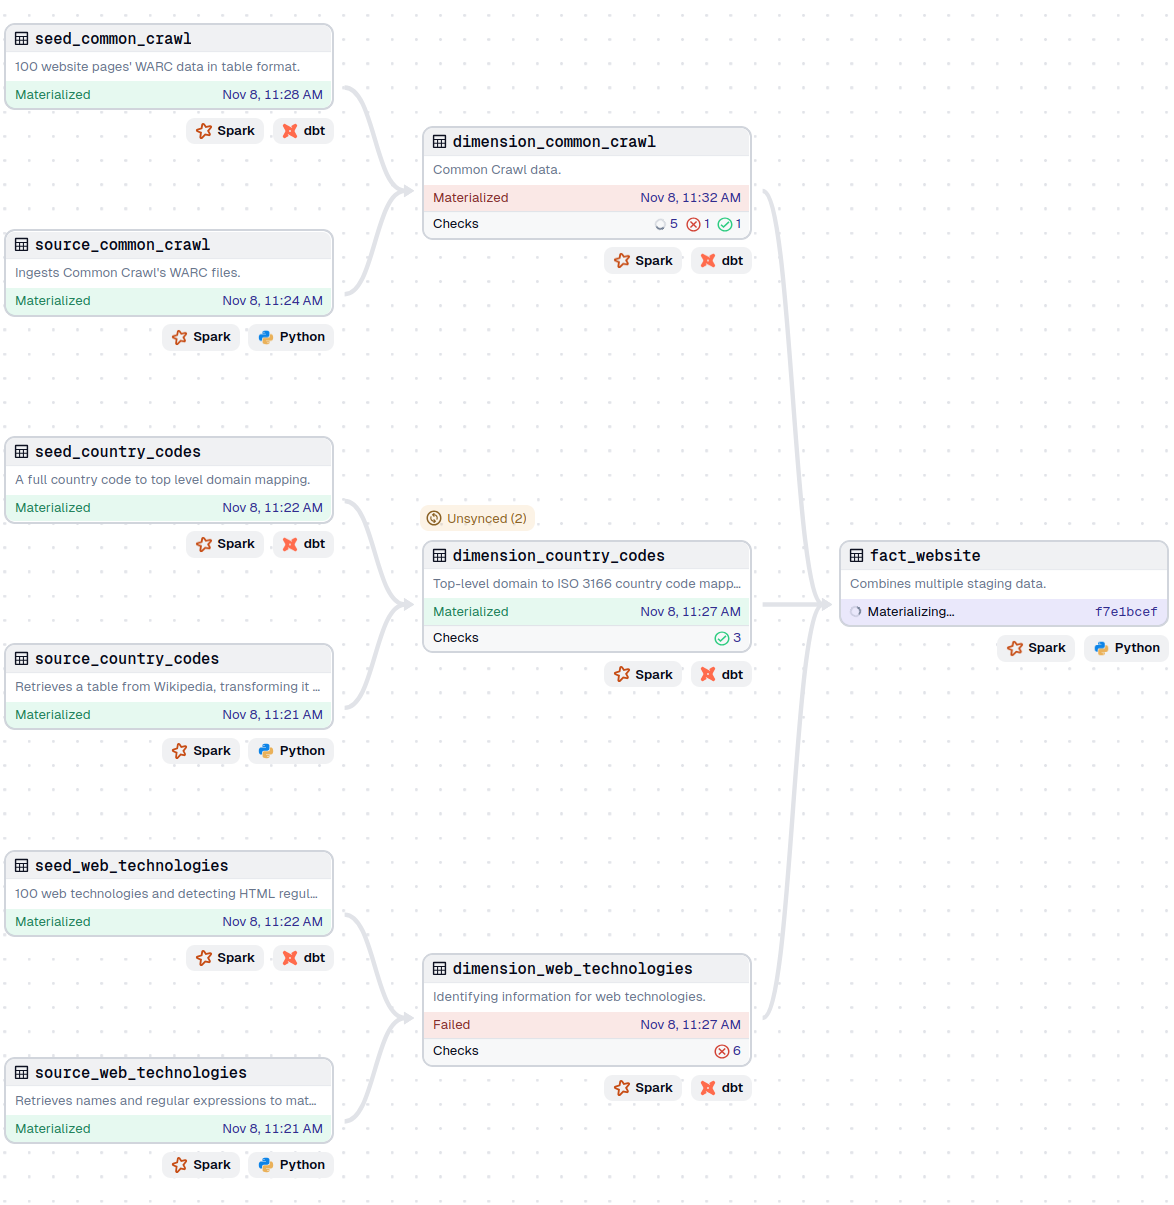
\includegraphics[width=\textwidth]{figures/dagster-white-ui-cut.png}
  \caption{Dagster dashboard of the Big Data pipeline.}
  \label{fig:implementation-dx-dashboard}
\end{figure}

A detailed examination of the country codes and web technologies assets will be left out to keep this section concise.
In brief, the country codes are fetched from a table on Wikipedia to demonstrate Pandas' basic \ac{html} extraction capabilities in \cref{lst:appendix-listings-pandas-tables}, and the data on web technologies is sourced from the \href{https://github.com/tunetheweb/wappalyzer/}{\textit{Wappalyzer}} project on GitHub.
Instead of crawling from Wikipedia, the \href{https://pypi.org/project/countrycode/}{\textit{countrycode}} Python package could be used.
Both methods are evaluated in \cref{sec:evaluation}.


\subsubsection{Visualization}
\label{sec:implementation-pipeline-visualization}

To generate graphs that visualize data from any table we create, we use \href{https://plotly.com/}{\textit{\ac{px}}}.
The implementation is straightforward: we define an example graph and then write it to a shared storage accessible by a web server.
We can then generate a link to the graph's web address and pass it as a result to Dagster's \ac{gui}.

\Cref{lst:implementation-pipeline-visualization-chart} demonstrates the generation of a choropleth map, as envisioned previously in \cref{fig:choropleth}.
First, an aggregate \ac{sql} statement is executed in a distributed manner via Spark (lines 2 to 6).
The resulting Spark DataFrame is converted into a Pandas DataFrame on line 7, as Spark DataFrames cannot be passed directly into \ac{px} functions.
The following lines configure the choropleth map.
Line 11 specifies the column that provides the country identifier in proper \href{https://www.iso.org/iso-3166-country-codes.html}{ISO 3166 alpha-3} format.
Lines 12 and 13 define the color scale used on the aggregate count, with \texttt{Viridis} chosen for optimal visibility for colorblind readers.
Lines 14 to 22 specify data displayed when hovering over countries in the map's \ac{html} version, providing detailed information that is useful for readers of the analysis in the next section.

\begin{listing}[H]
\begin{minted}{python}
def get_chart_fact_uri_choropleth():
  df_spark = SparkManager.spark.sql("""
    SELECT iso_3166_alpha3, country, COUNT(uri)
    FROM marts.fact_website
    GROUP BY iso_3166_alpha3, country
  """)
  df_pandas = df_spark.toPandas()

  graph = px.choropleth(
    df_pandas,
    locations="iso_3166_alpha3",
    color="count(uri)",
    color_continuous_scale=px.colors.sequential.Viridis,
    hover_data=["count(uri)", "iso_3166_alpha3"],
    hover_name="country",
    labels={
      "count(uri)": "Count",
      "iso_3166_alpha3": "ISO 3166-1 alpha-3 code",
    },
  )
  graph.update_traces(marker_line_color="white")
  graph.update_layout(
    title_text="Website Count by Country",
  )

  return graph
\end{minted}
\caption{Chart generation using Plotly.}
\label{lst:implementation-pipeline-visualization-chart}
\end{listing}

To separate transformations from visualizations, all graphs are generated by a new Dagster asset named \texttt{charts}.
Alternatively, each existing asset could be extended to output relevant graphs.

\Cref{lst:implementation-pipeline-visualization-charts} shows the new Dagster asset for chart generation.
Lines 7 to 9 exemplarily reference the chart's getter function, defined in the preceding \cref{lst:implementation-pipeline-visualization-chart}, keyed by a file name.
For each such combination -- many more are omitted here for brevity -- the graph is generated and written to storage in lines 11 to 13.

\begin{listing}[H]
\begin{minted}{python}
@asset(
  kinds={"python", "plotly"},
  deps=[fact_website],
)
def charts(context: AssetExecutionContext):
  web_server_directory = os.path.join(os.sep, "srv", "charts")
  charts = {
    "chart_fact_uri_choropleth": get_chart_fact_uri_choropleth, # ...
  }

  for file_name, chart_function in charts.items():
    chart = chart_function()
    chart.write_html(os.path.join(web_server_directory, file_name + ".html"))

  context.add_output_metadata(
    {
      "Charts": MetadataValue.url(
        "https://charts.big-data-pipeline.uni-kassel.dev/"
        if IS_KUBERNETES
        else "http://0.0.0.0:3001/"
      ),
    },
  )
\end{minted}
\caption{Chart output with dashboard linking.}
\label{lst:implementation-pipeline-visualization-charts}
\end{listing}

Finally, the \ac{url} to view the generated charts is added as output metadata to the Dagster asset, allowing convenient access through the Dagster workflow \ac{gui}, as shown in \cref{fig:implementation-visualization-metadata}.
The \ac{url} where the web server is available differs between development and production environments, as specified in lines 18 to 20 of \cref{lst:implementation-pipeline-visualization-charts}.

\begin{figure}[H]
  \centering
  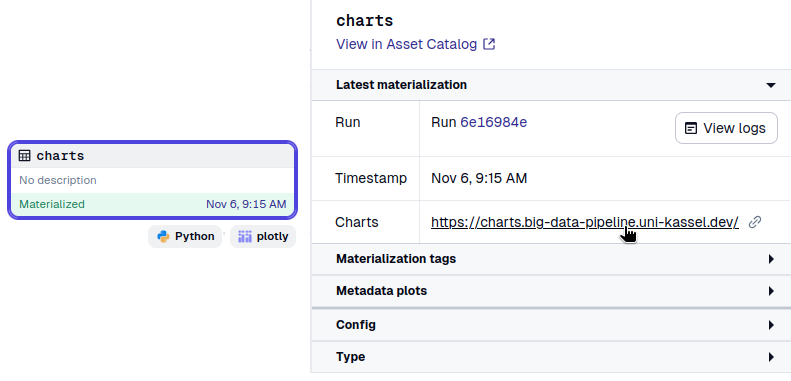
\includegraphics[width=0.85\textwidth]{figures/dagster-asset-metadata.png}
  \caption{The web server link in the \texttt{chart} asset's materialization metadata.}
  \label{fig:implementation-visualization-metadata}
\end{figure}

\subsubsection{Orchestration}
\label{sec:implementation-pipeline-orchestration}

To complete the Dagster service implementation, we define a multistage Dockerfile that allows building container images for both development and production, shown in \cref{lst:appendix-listings-dockerfile}.
This Dockerfile defines five stages for build time efficiency and \ac{dx}:

\begin{enumerate}
  \item \textbf{base-image} defines environment variables, installs \ac{os} dependencies, and sets up a rootless user, serving as the basis for stages 2 and 3.
  \item \textbf{development} builds on stage 1. It configures an entrypoint, a command, volumes, and a port to expose, all for development only. This setup allows the project to run in a container during development, ensuring a predictable environment\footnote{Refer to the open \href{https://containers.dev/}{\textit{Development Container}} specification for more on this concept.}.
  \item \textbf{prepare} also builds on stage 1, skipping stage 2. It installs Python dependencies and is intended as an incrementally extended base image for subsequent stages. For example, a \texttt{lint} stage could be added as a sibling to \texttt{build}, based on the \texttt{prepare} stage, to validate code formatting using \href{https://docs.astral.sh/ruff/}{\textit{Ruff}}.
  \item \textbf{build} builds on stage 3, copies all source code into the image, and builds the dbt project through Dagster's dbt extension.
  \item \textbf{production} builds on stage 4, installing \ac{os} dependency updates as the root user before reverting to the rootless user, and declares the command, volume, and port for production. The default command runs Dagster's webserver, but this command can be overridden in the container orchestrator's configuration to run Dagster's daemon for sensor, backfill, and scheduler support as well.
\end{enumerate}

In addition to enabling the building of development and production images, this image can serve as a substitute for a proprietary \ac{ci} pipeline.
Only minimal code needs to be written in a proprietary \ac{ci} pipeline format to initiate the Dockerfile's build process.

To build the development image, the command shown on line 1 of \cref{lst:dockerfile-build} can be executed in the working directory containing the Dockerfile.
The command on line 2 builds the final stage defined in the Dockerfile, along with all stages on which the final stage transitively depends (i.e., all stages except the \texttt{development} stage).

\begin{listing}[H]
\begin{minted}{bash}
docker build -t dargmuesli/web-kraken:dev --target development . # development
docker build . # ci
\end{minted}
\caption{Commands to build the Dockerfile.}
\label{lst:dockerfile-build}
\end{listing}

With the development image now available for our Dagster service, we can circle back to the Docker Compose infrastructure definitions in \cref{sec:implementation-infrastructure} and define a configuration for the Dagster service.
\Cref{lst:compose-dagster} shows this configuration.
On line 6, the image generated by the command on line 1 of \cref{lst:dockerfile-build} is used.
The Dagster service is also configured to start only when the Spark master and workers are available, ensuring that workflows cannot run while the Spark master or workers are still booting (lines 3 to 5).
Ports used by the Dagster container are \texttt{3000} for the main workflow \ac{gui}, \texttt{4040} for the Spark driver \ac{gui}, and \texttt{7777} for Spark's driver \ac{api} (lines 11 to 14).
Two volumes persist Dagster's workflow run data, including logs and generated charts (lines 16 to 18 and 21 to 23).
Two additional volumes, mounting a host directory into the container, enable a true Development Container experience: changes in the source code are directly accessible to Dagster without requiring a service restart (lines 19 and 20).

\begin{listing}[H]
\begin{minted}{yaml}
services:
  dagster:
    depends_on:
      - spark-iceberg
      - spark-iceberg-worker
    image: dargmuesli/web-kraken:dev
    environment:
      - AWS_ACCESS_KEY_ID=admin
      - AWS_SECRET_ACCESS_KEY=password
      - AWS_REGION=us-east-1
    ports:
      - 3000:3000
      - 4040:4040
      - 7777:7777
    restart: unless-stopped
    volumes:
      - dagster_data:/home/rootless/dagster
      - httpd_data:/srv/charts
      - ./orchestration:/srv/app
      - ./transformation:/srv/transformation
volumes:
  dagster_data: {}
  httpd_data: {}
\end{minted}
\caption{Docker Compose definition for Dagster.}
\label{lst:compose-dagster}
\end{listing}

With this, we have implemented all services for scheduling via Docker Compose.
For production, we need to define Kubernetes resources, as described in the next section.


\subsection{Deployment}
\label{sec:implementation-deployment}

The services from \cref{sec:implementation-infrastructure} and \cref{sec:implementation-pipeline-orchestration} were defined for development deployment using Docker Compose.
This section outlines the necessary modifications for production deployment using Kubernetes.

The bulk of the migration from a \texttt{docker-compose.yaml} file to Kubernetes resource definitions can be handled with Kompose, which translates each declaration individually.
However, not every declaration can or should be translated in isolation.

For example, Kubernetes' concept of \texttt{pods} allows the \texttt{dagster} container definition to be merged with the \texttt{httpd} container definition within the same pod.
This merging into a single pod is necessary, as the shared storage currently only supports the \texttt{ReadWriteOnce} access mode, which prevents mounting this volume for multiple deployments\footnote{\texttt{ReadWriteMany} is available starting with Harvester v1.4.0-rc2, paired with Rancher v2.8.8 (csi-driver 0.1.19) and v2.9.2 (csi-driver 0.2.0)~\cite{TachunLin2024}.}.
Additionally, no entrypoint script is needed for \texttt{httpd} to correct filesystem permissions for the mounted shared storage, as Kubernetes allows specification of the desired filesystem permissions directly.

To ensure a correct order of resource deployment, we define several custom resource definitions as detailed in the following enumeration.

\begin{enumerate}
  \item \texttt{minio}
  \begin{enumerate}
    \item \texttt{Secret} \textbf{minio-secrets} defines S3 secrets and MinIO's \ac{gui} credentials.
    \item \texttt{PersistentVolumeClaim} \textbf{minio-data} reserves 1~TiB of storage.
    \item \texttt{Service} \textbf{minio} makes ports \texttt{9000} and \texttt{9001} accessible.
    \item \texttt{Deployment} \textbf{minio} defines the MinIO container with dependencies on the previously defined secrets and volume.
    \item \texttt{Job} \textbf{minio-client} is the equivalent of the MinIO client definition from \cref{lst:minio-client-compose} that initializes a bucket once.
  \end{enumerate}

  \item \texttt{rest}
  \begin{enumerate}
    \item \texttt{Service} \textbf{rest} makes port \texttt{8181} accessible. It must be defined before the \texttt{Deployment} as the catalog implementation requires knowledge of the assigned address at boot, which Kubernetes makes available to containers through environment variables once a \texttt{Service} is assigned.
    \item \texttt{Deployment} \textbf{rest} defines the \texttt{rest} container and additionally sets the \texttt{REST\_PORT} environment variable to override the environment variable of the same name automatically set by Kubernetes due to the preceding \texttt{Service} definition.
  \end{enumerate}

  \item \texttt{spark-iceberg-configmap}
  \begin{enumerate}
    \item \texttt{ConfigMap} \textbf{spark-iceberg-defaults} prepares the Spark defaults for usage by both the Spark master and Spark workers.
  \end{enumerate}

  \item \texttt{spark-iceberg-master}
  \begin{enumerate}
    \item \texttt{ConfigMap} \textbf{spark-iceberg-master} adds the Spark master's entrypoint script.
    \item \texttt{Service} \textbf{spark-iceberg} makes ports \texttt{7077}, \texttt{8080}, \texttt{8888}, and \texttt{10000} accessible.
    \item \texttt{Deployment} \textbf{spark-iceberg} defines the Spark master container, mounting its entrypoint with \texttt{0744} permissions so it is executable.
  \end{enumerate}

  \item \texttt{spark-iceberg-worker}
  \begin{enumerate}
    \item \texttt{ConfigMap} \textbf{spark-iceberg-worker} adds the Spark workers' entrypoint script.
    \item \texttt{Service} \textbf{spark-iceberg-worker} makes ports \texttt{7878} and \texttt{8787} accessible.
    \item \texttt{StatefulSet} \textbf{spark-iceberg-worker} defines seventeen Spark worker containers, one less than the nodes available in the cluster, as one node should remain hosting only the Spark master\footnote{Node affinity will be evaluated in \cref{sec:evaluation}}. The \texttt{StatefulSet} also mounts its entrypoint with filesystem permissions that make it executable.
  \end{enumerate}

  \item \texttt{dagster}
  \begin{enumerate}
    \item \texttt{PersistentVolumeClaim} \textbf{dagster-data} reserves 1~GiB of storage for Dagster's status management, such as log persistence of workflow runs.
    \item \texttt{PersistentVolumeClaim} \textbf{httpd-data} reserves 1~GiB of storage for charts generated to visualize insights into the stored dataset.
    \item \texttt{Service} \textbf{dagster} makes ports \texttt{3000}, \texttt{4040}, \texttt{7777}, and \texttt{7878} accessible.
    \item \texttt{Service} \textbf{dagster-httpd} makes port \texttt{3001} accessible.
    \item \texttt{Deployment} \textbf{dagster} mounts volumes with appropriate permissions that allow writes for the \texttt{rootless} user and defines the Dagster container, along with a Dagster daemon and a web server sidecar container. The web server sidecar makes the charts accessible via the web for analysis in \cref{sec:analysis}.
  \end{enumerate}

  \item \texttt{ingress}
  \begin{enumerate}
    \item \texttt{Ingress} \textbf{ingress} makes the pipeline's Dagster dashboard available at \newline\texttt{big-data-pipeline.uni-kassel.dev}. The web server hosting the charts, the Spark driver's \ac{gui}, and MinIO's dashboard are accessible at the same address, prefixed by \texttt{charts.}, \texttt{driver.}\footnote{The driver is only available while a Spark job is running.}, or \texttt{minio.}, respectively. For all addresses, the cluster's certificate manager is configured to fetch \ac{tls} certificates from \href{https://letsencrypt.org/}{\textit{Let's Encrypt}}.
  \end{enumerate}
\end{enumerate}


\newpage
\acresetall
\cleardoublepage
\section{Analysis and Results}
\label{sec:analysis}

Our pipeline ingested 600 \ac{warc} files: 300 files for responses with a successful status code and 300 files for responses with various other status codes.
The \ac{regex} \texttt{\textasciicircum.+-0000(0|1|2)\textbackslash .warc\textbackslash .gz\$} was used to select these 300 files from each data subset.
Each \ac{warc} file containing successful responses is approximately 900~MiB in size, while each file containing non-successful responses is about 29~MiB.
Thus, all compressed \ac{warc} files with successful status codes amount to approximately 264~GiB, and those with non-successful status codes to approximately 8~GiB.
The total data size fetched from Common Crawl is roughly \textbf{272~GiB}.
The total number of crawled responses ingested is \textbf{7,440,858}.

After transformations, specifically the \ac{cctld} selection, the \texttt{fact\_website} table contains \textbf{3,117,139} entries, 4,323,719 fewer than those ingested into the bronze layer.
This means that 41.9\% of all crawled websites fetched used a \ac{cctld}.

After a full pipeline run, the MinIO \ac{gui} and the \texttt{df} Linux \ac{cli} tool report 159.3~GiB of mounted storage space in use.

In the following section, we will discuss the pipeline's runtime performance.
Then, we will present the results of exemplary analyses on the ingested Common Crawl data as well as on combinations of data from different sources.


\subsection{Pipeline performance}
\label{sec:analysis-pipeline}

All Dagster assets exhibit varying execution times.
\Cref{tab:analysis-dataset-asset-times} details the durations of asset executions measured over a full pipeline run.

\begin{table}[H]
    \centering
    \begin{tabular}{|c|c|c|c|c|}
    \hline
    \textbf{Namespace} & \textbf{Type} & \textbf{Name} & \textbf{Duration} & \textbf{Configuration} \\
    \hline
    raw & seed & common\_crawl & 00:06:50 & - \\
    raw & seed & country\_codes & 00:02:01 & - \\
    raw & seed & web\_technologies & 00:02:00 & - \\
    raw & source & common\_crawl & 36:20:02 & 200responses \\
    raw & source & common\_crawl & 03:21:18 & non200responses \\
    raw & source & country\_codes & 00:00:47 & - \\
    raw & source & web\_technologies & 00:00:43 & - \\
    staging & dimension & common\_crawl & 00:04:39 & - \\
    staging & dimension & country\_codes & 00:03:02 & - \\
    staging & dimension & web\_technologies & 00:04:06 & - \\
    marts & fact & website & 02:27:29 & - \\
    - & - & charts & 00:04:47 & - \\
    \hline
    \end{tabular}
    \caption{Asset execution times.}
    \label{tab:analysis-dataset-asset-times}
\end{table}

The larger \texttt{common\_crawl} seed (2.7~MB) takes almost seven minutes to load, while the smaller \texttt{country\_codes} and \texttt{web\_technologies} seeds (below 15~kB each) take around two minutes to load.
Loading these smaller seeds takes longer than expected, given that large volumes of data can be processed relatively quickly; if it is possible to download, decompress, process, compress, and persist over 250~GiB of data within 36 hours using the \texttt{common\_crawl} asset, a local \ac{csv} file of 2.7~MB should theoretically load in under a second.

Closer inspection of the dbt seed run reveals that the majority of time is consumed by dbt's startup (one minute), processing (half a minute for small files, four minutes for larger files), and shutdown (an additional half minute).

The exact cause of these long durations remains uncertain, though debug information indicates that most of the time is spent after \texttt{Close} commands on Spark connections are logged.
This delay does not occur when using a \texttt{session} connection instead of a \texttt{thrift} connection in dbt's profiles configuration, as shown in \cref{lst:implementation-pipeline-transformation-dbt-profiles}.
However, using a \texttt{session} connection can cause issues in PySpark's \ac{sql} statements due to unescaped characters within the seed sources, such as carets.

Further research indicates that dbt, in conjunction with its Spark adapter, initially builds a cache of all schema and table metadata.
dbt attempts to execute a \texttt{SHOW TABLE EXTENDED} \ac{sql} command, which is unsupported in Spark's Data Source V2 \ac{api} in versions prior to Spark \texttt{4}\footnote{Spark \texttt{4} is not yet released at the time of writing, although a preview was released on 2024-09-26.}.
Consequently, dbt falls back on \texttt{SHOW TABLE} and \texttt{DESCRIBE TABLE} statements, which become increasingly time-consuming as the number of schemas and tables grows.

Sourcing a table from an \ac{html} page and \ac{json} files from GitHub, as done for country codes and web technologies respectively, takes around 40 seconds.
Most of that time passes while the Spark session initializes.

Each test run by dbt requires about 20 seconds to complete.
For \texttt{dimension\_common\_crawl}, this results in a total of 2:19 minutes for seven checks.
The same checks take five to ten seconds on a cold PySpark session and under two seconds on a warm PySpark session\footnote{A cold session is one that has not run any queries since startup, whereas a warm session has already run a query.}.

Materializing the \texttt{website} fact table takes about 2.5~h, which is more than 14 times faster than the ingestion of Common Crawl data alone.
This demonstrates that operations on data stored within local table structures are highly efficient with respect to performance, even when running more complex \texttt{JOIN} operations and extensive \ac{regex} pattern matching.

Finally, the 17 \ac{px} charts materialize in under five minutes.
While most generated chart files have a size of approximately 5~MB, some include data points for all table rows, resulting in file sizes between 50~MB and 100~MB.
If more data is added to these tables, the chart generation strategy for those large chart files would need to change.
Even now, opening these large chart files locally in a modern browser on an ordinary computer takes more than ten seconds.

A typical log output of a Dagster asset's function run, including time measurements, is shown in \cref{lst:appendix-listings-spark-logs}.
The time measurements stem from the decorator defined in \cref{lst:dagster-utility-performance-measurement} for performance assessment.
This log output shows sub-second durations for data stream fetching (lines 1, 2, and 4).

From lines 6 to 24, the log shows Spark initializing with the \ac{jar} files required for Iceberg table format support on S3 object storage.
The following lines display the Spark job running.
The warnings can be ignored, as we do not want to eliminate website \ac{html} payloads above 1000~KiB from our dataset and splitting the \ac{html} would not be trivial.
The first write execution (68.0258~s, line 26) always takes longer than subsequent writes (e.g., 42.6831~s, line 28).
Write times would be considerably less if we simply appended data, without removing duplicates first.


\subsection{Dataset analysis}
\label{sec:analysis-dataset}

The following figures visualize key metrics of our dataset.
The figures are generated using \ac{px} in functions such as the one shown in \cref{lst:implementation-pipeline-visualization-chart}.

All charts in this thesis are images of \ac{html} documents that allow interactivity, such as hovering over fields to show details, clicking on legend elements to hide respective fields, and zooming in and out of graph areas.
The first figure, \cref{fig:analysis-dataset-chart_source_charset_pie}, shows a mouse hovering over a field as an example of interactivity; all subsequent graphs are shown without such overlays.

We first inspect the bronze layer's Common Crawl dataset as ingested by the methods outlined in \cref{sec:implementation-pipeline-ingestion}.
This step is important as it allows us to validate the source data quality.
On this basis, we then proceed with a more detailed analysis of country-specific web technology usage as envisioned in \cref{sec:design-envisioned-result}.


\subsubsection{Analysis of source data}
\label{sec:analysis-dataset-source}

After the ingestion of all 600 \ac{warc} files, the silver layer's staging view was materialized, and one of its checks failed.
This test failure was due to only two entries out of more than seven million, which had status codes of \texttt{706} and \texttt{999}.
We defined a custom macro in \texttt{dbt}, as shown in \cref{lst:implementation-pipeline-transformation-dbt-macro}, that allowed us to catch unexpected data.

At the time of writing, the pages that returned the implausible status codes to Common Crawl now return the expected status code of \texttt{200} to a standard browser request.
The web servers may be configured to respond differently to requests originating from Common Crawl, either due to a technical flaw or intentionally.

These outlier status codes were caught by coincidence, thanks to our previous exemplary test definition.
A guess-based approach for testing would be inefficient to continue, which is why we examine data distributions in the following graphs.
We aim to use visual representations to gain insights into the quality of our data.

The data source provider, Common Crawl, also offers statistics on their dataset, as referenced in \cref{sec:related-work-big-data-datasets}.
This allows for comparisons between the full dataset, as analyzed by Common Crawl, and our subset of it, which will be discussed in the following chapter, \cref{sec:evaluation}.

The first metric we inspect is the \ac{http} charset distribution, i.e., a distribution of character encodings that map page contents' bytes to their text representation.
As displayed in \cref{fig:analysis-dataset-chart_source_charset_pie}, the vast majority (87.6\%) of \ac{http} responses specify \texttt{utf-8} as charset, representing 6,516,178 pages.
The next most commonly specified charset is not \texttt{iso-8859-1}, as might be expected if a charset were mandatory, but an empty charset specification (8.72\%).
\texttt{iso-8859-1}, also known by its \href{https://home.unicode.org/}{\textit{Unicode}} block name \textit{Latin-1}, is a single-byte encoding as opposed to \texttt{utf-8}'s multibyte encoding and ranks third (2.51\%).
For readability, we group all charsets with a frequency below 0.1\% into a category named \texttt{Other}, which comprises around 0.7\% of all charset specifications.

\begin{figure}[H]
    \centering
    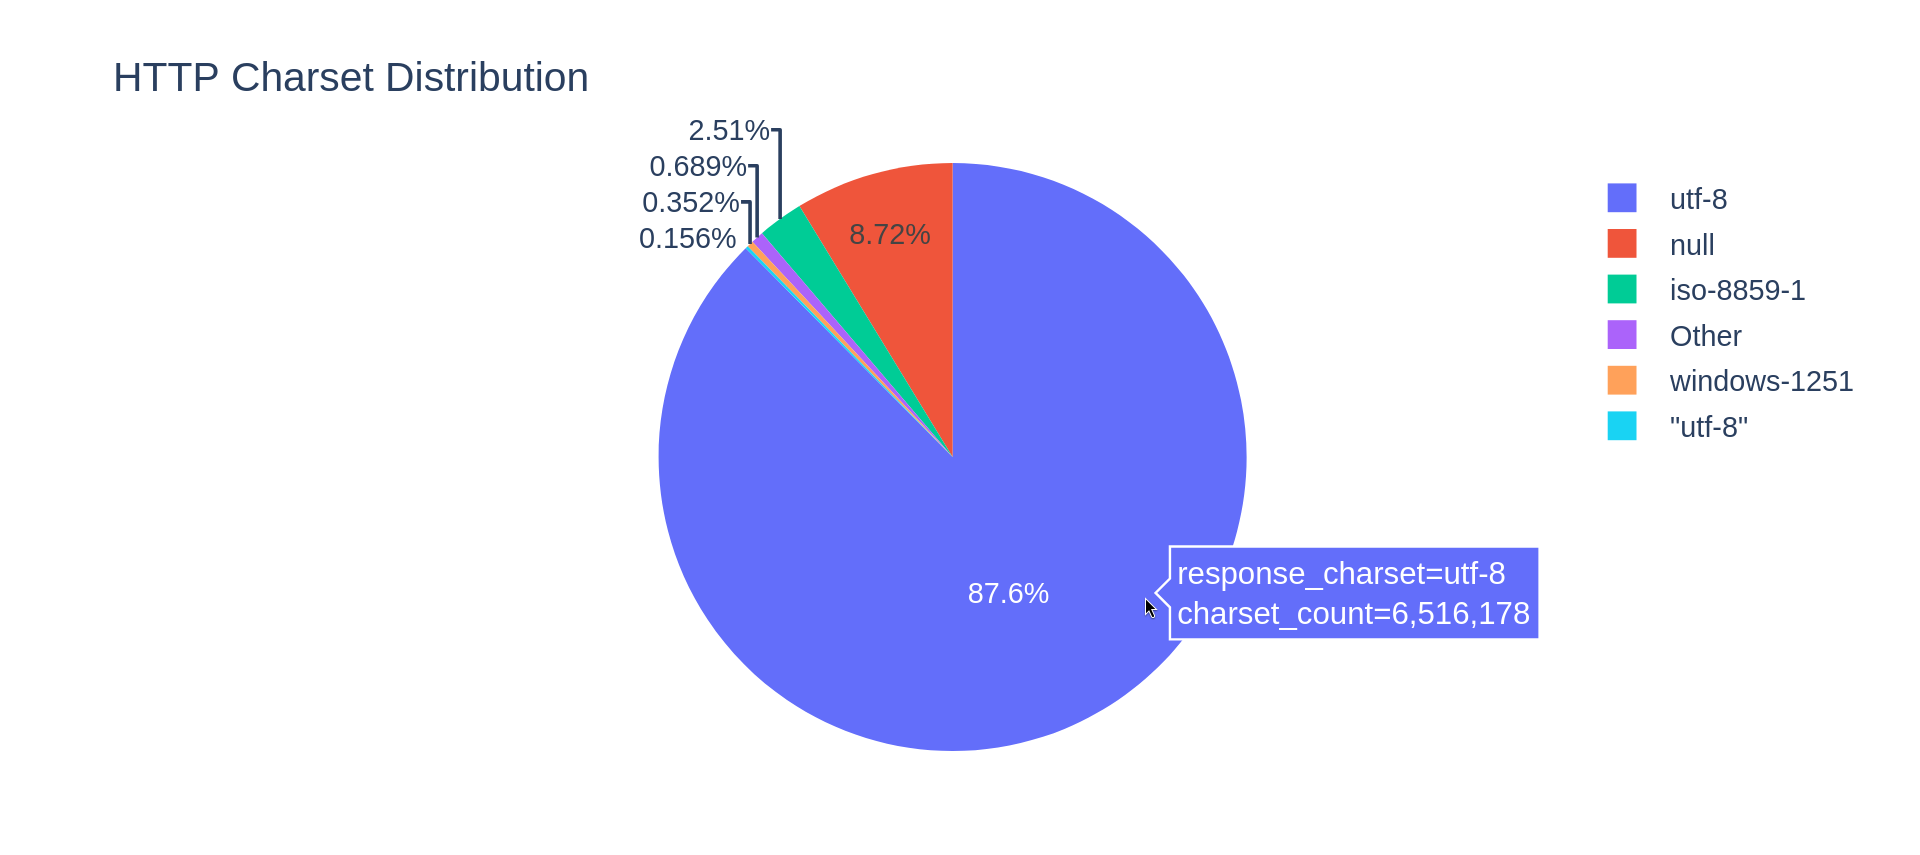
\includegraphics[width=\textwidth]{figures/charts/large/chart_source_charset_pie.png}
    \caption{Charset distribution with hover overlay.}
    \label{fig:analysis-dataset-chart_source_charset_pie}
\end{figure}

\Cref{fig:analysis-dataset-chart_source_charset_pie} already provides an important insight into data quality: the fourth most common charset among all responses with a specified charset is \texttt{"utf-8"} (i.e., \texttt{utf-8} with quotation marks).
While this formatting is likely not compliant with specifications, it may go undetected by web developers as clients could work around such common misconfigurations.
However, this hypothesis has not been researched further.

If future research shows such client workarounds to be common, a possible data quality improvement could be to remove quotation marks in the view definition set in \cref{lst:implementation-pipeline-transformation-dbt-model} so that quoted variants are not counted separately.
A second reason supporting this improvement could be that modern browsers fall back to \texttt{utf-8} when encountering an unexpected charset, such as one with quotes.

To explore the distribution of charsets besides \texttt{utf-8} and \texttt{null}, we exclude these most common encodings and obtain the graph shown in \cref{fig:analysis-dataset-chart_source_charset_pie_excluding_utf8}.
In this graph, all charsets that appear in less than 0.8\% of the remaining cases, i.e. less than 0.03\% of all ingested websites, are grouped into the \texttt{Other} category.
Besides the quoted variant of \texttt{utf-8}, another variant specified as \texttt{utf8} is now visible, occurring in 3,803 of the ingested websites (0.05\%).

\begin{figure}[H]
    \centering
    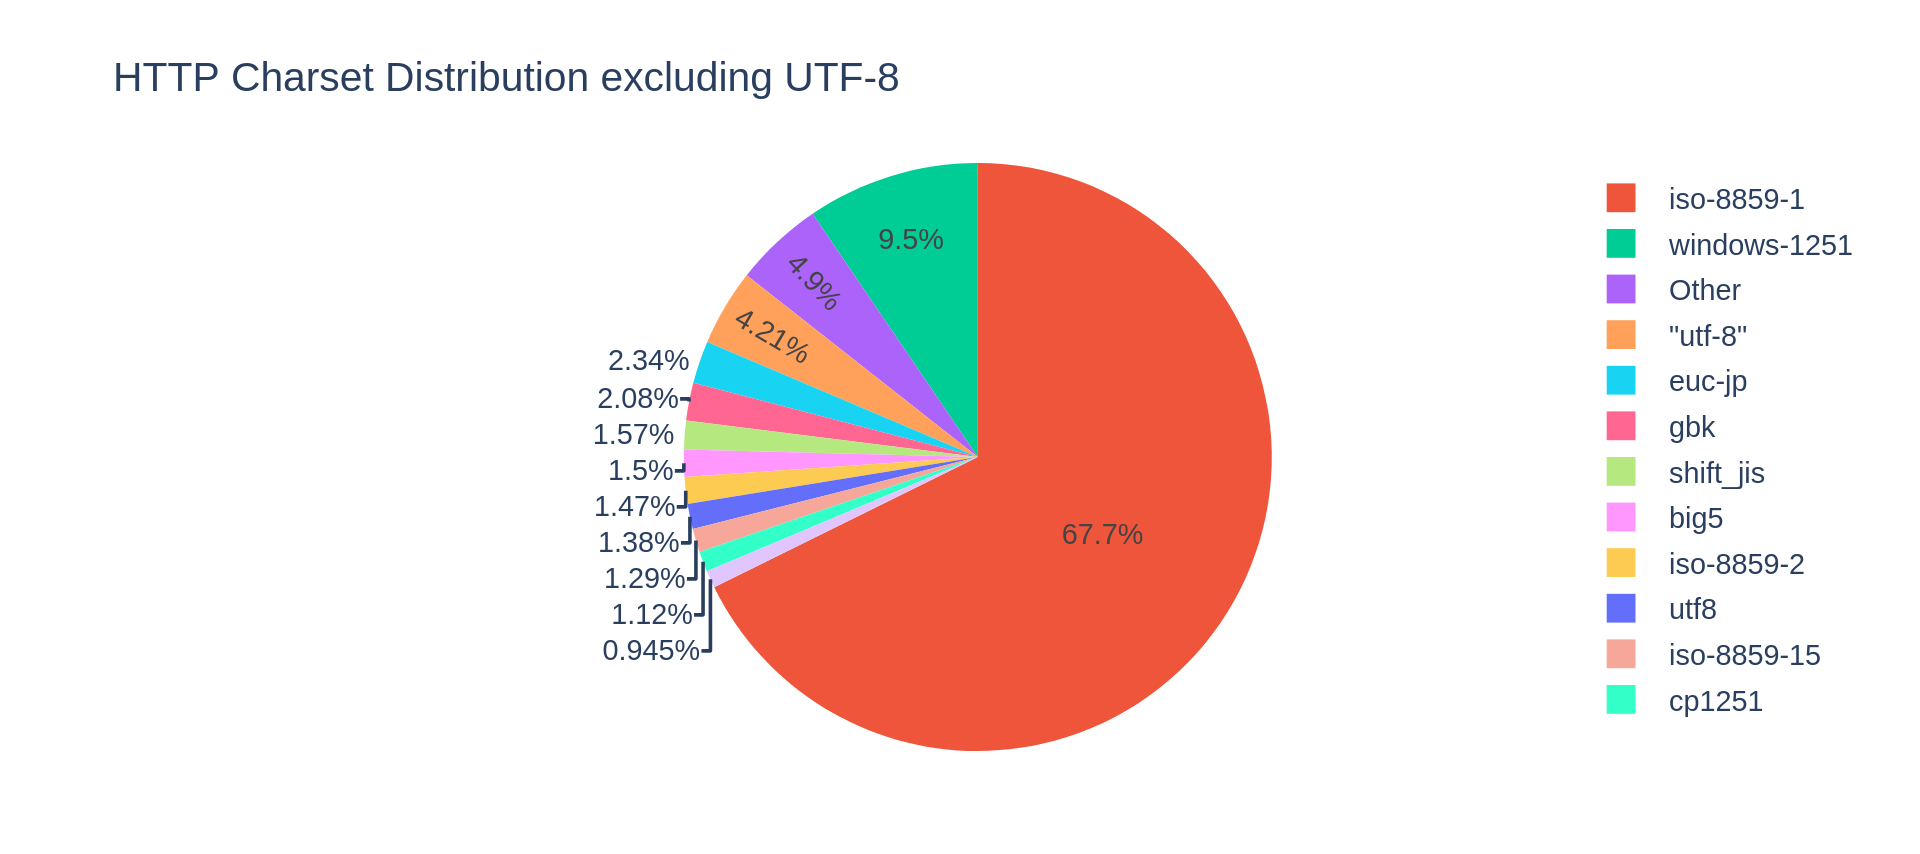
\includegraphics[width=\textwidth]{figures/charts/large/chart_source_charset_pie_excluding_utf8.png}
    \caption{Charset distribution, excluding \texttt{UTF-8}.}
    \label{fig:analysis-dataset-chart_source_charset_pie_excluding_utf8}
\end{figure}

Now that we are aware of the various charsets in use, we analyze website size next, as a website's size depends on the amount of content and, to some extent, on the charset used.

\Cref{fig:analysis-dataset-chart_source_payload_size_bar_count} shows the distribution of \ac{http} payload size ranges.
There are 2.9~million websites with a payload size of zero to 50~kB and about half as many in each successive 50~kB range, except for websites in the 1~MB to 1.05~MB range.
Since the graph does not show websites larger than 1.05~MB, it appears that there is a size limit for each website in the Common Crawl dataset of 1~MiB.

The 1~MB to 1.05~MB range stands out as the only range with a higher count of websites than any of the ranges of smaller payload size.
Presumably, there might be a technical reason that limits website payloads surpassing the 1~MiB boundary, so they appear as 1~MiB in size, though intended to be larger.
There are 138 thousand pages in our dataset that fall in the 1~MB to 1.05~MB range, while only 14 thousand pages fall in the adjacent 0.95~MB to 1~MB range.

\begin{figure}[H]
    \centering
    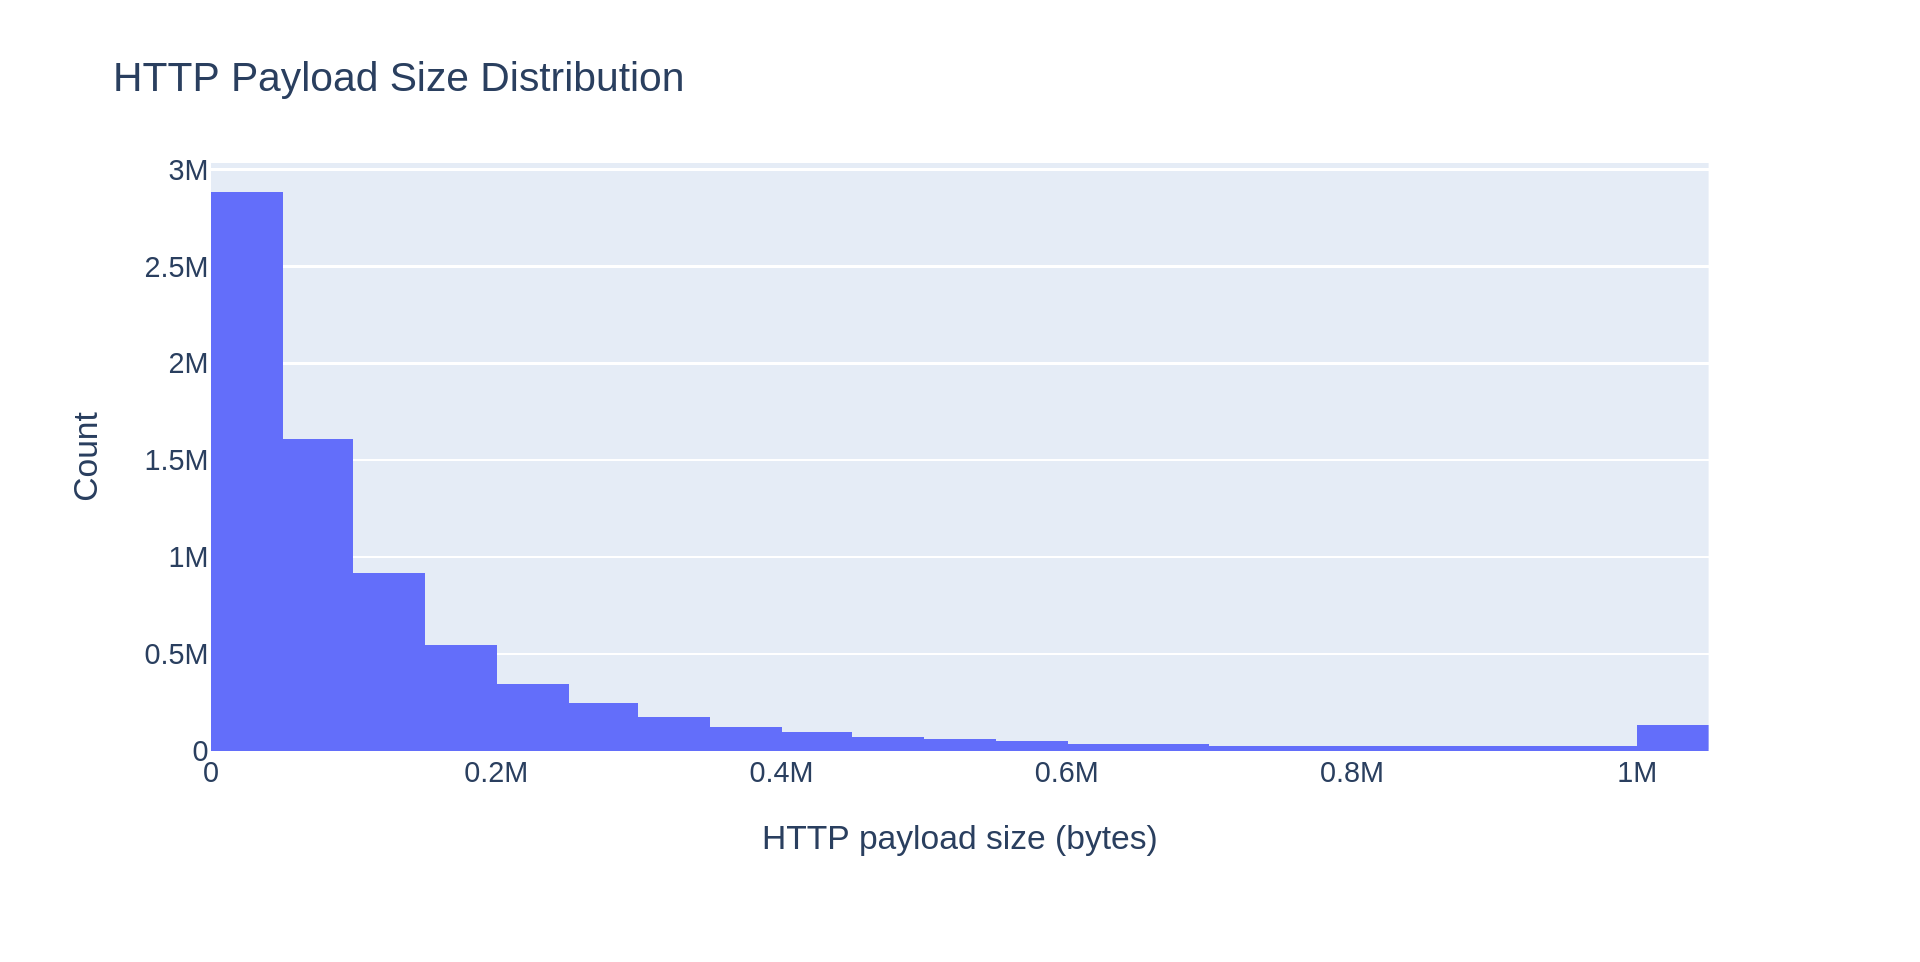
\includegraphics[width=\textwidth]{figures/charts/large/chart_source_payload_size_bar_count.png}
    \caption{Payload size distribution.}
    \label{fig:analysis-dataset-chart_source_payload_size_bar_count}
\end{figure}

A scatter plot provides another perspective on the correlation between the byte size and decoded character length of a website.
\Cref{fig:analysis-dataset-chart_source_payload_size_scatter_payload_length} shows this correlation.
Beyond the intuitive observation that no website has fewer characters than bytes, there is a notable variance in the relationship between bytes transmitted and decoded character length.

While single-byte encodings, such as \texttt{ascii} or \texttt{iso-8859-1}, appear only along the diagonal with a slope factor of one, multi-byte encodings allow multiple transmitted bytes to represent a single character.
However, there is no distinct secondary axis with a different slope factor visible in the graph, which would indicate that a charset requires a fixed byte count for each character.
Instead, multibyte character encodings appear to allow one-to-one mappings between a byte and a character as well as many-to-one mappings of multiple bytes to a character.
Furthermore, there seems to be an upper limit within the detected charsets for the number of bytes that can be decoded into a single character, apparent from the empty area in the top left.
Additionally, a horizontal line of dots can be seen at the 1~MiB payload size level, which we already observed in \cref{fig:analysis-dataset-chart_source_payload_size_bar_count}.

Regarding data quality and interpretation accuracy, it is essential to consider the representativeness of each part of the dataset inspected.
For example, \cref{fig:analysis-dataset-chart_source_payload_size_bar_count} shows that websites with smaller payload sizes are more common than websites with larger payload sizes.
This pattern is reflected in the higher density of dots in the lower left area of the graph behind \cref{fig:analysis-dataset-chart_source_payload_size_scatter_payload_length}.
Without considering this context, one might erroneously conclude that less common charsets are specified more frequently by smaller websites, as more dots with colors other than the color for the \texttt{utf-8} charset are visible in the lower left corner.
A different chart, potentially normalizing by charset frequency, would be useful to analyze the average payload size for each charset.

\begin{figure}[H]
    \centering
    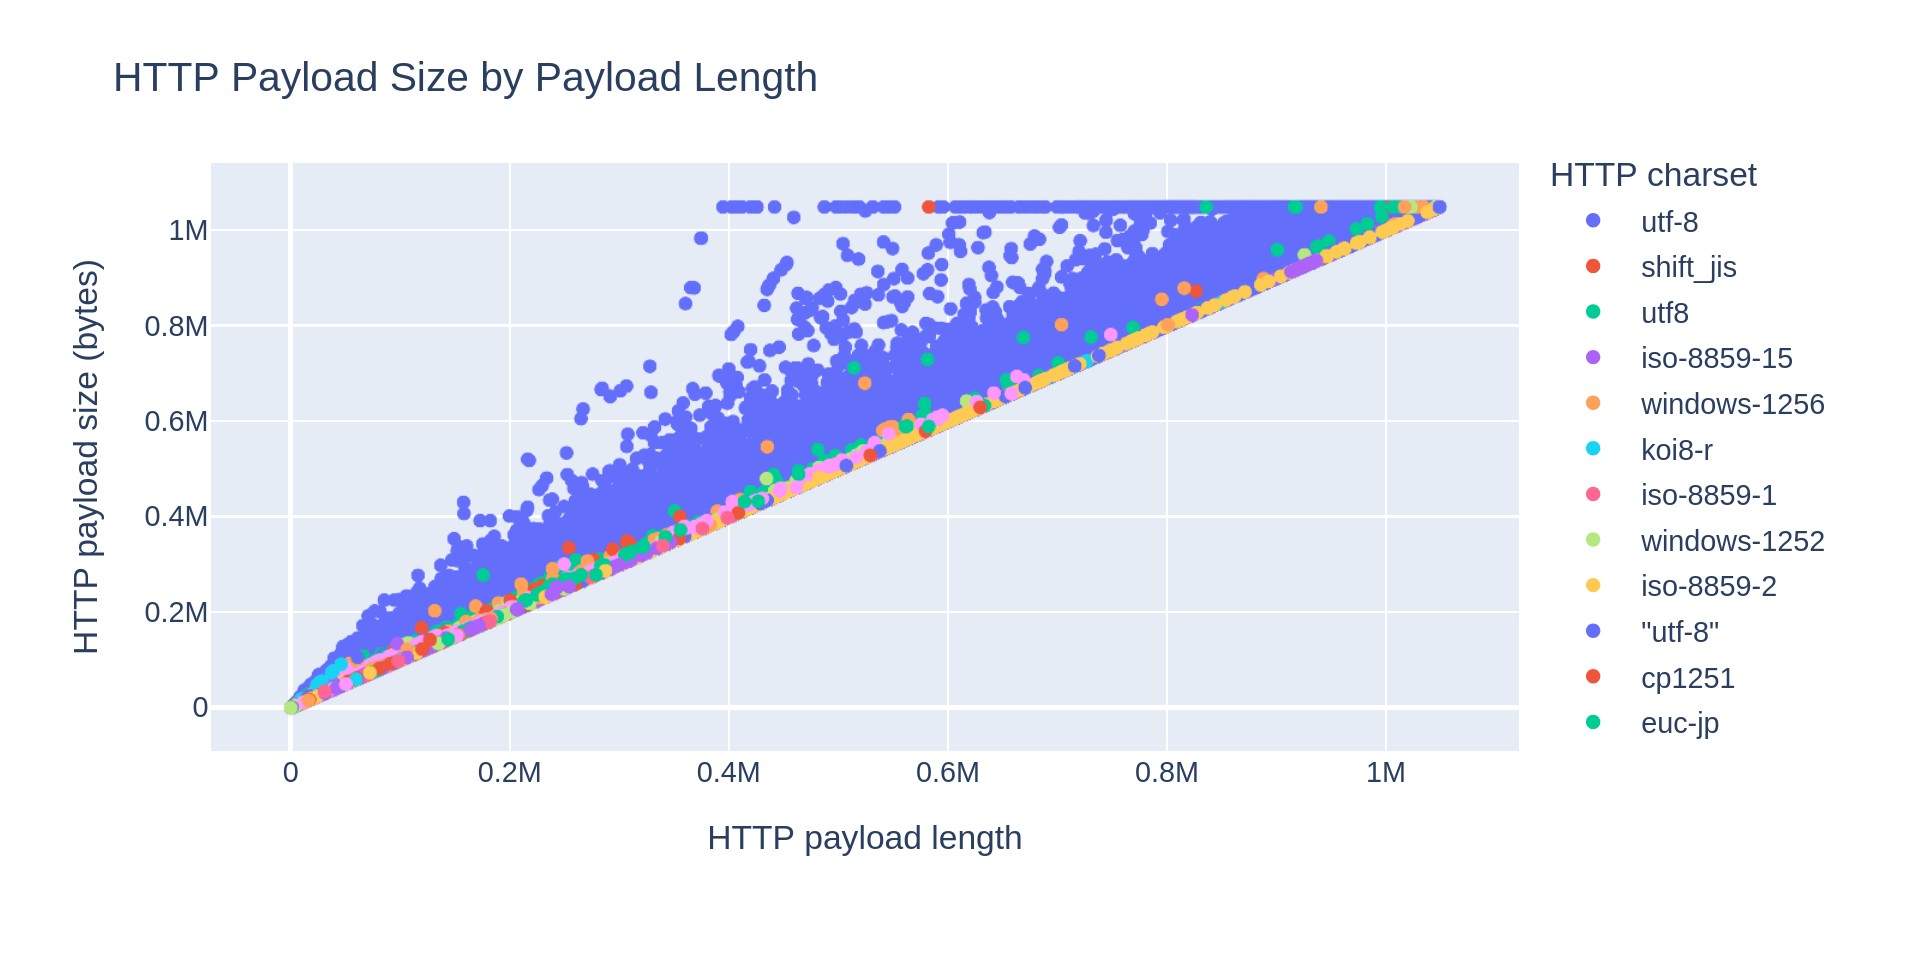
\includegraphics[width=\textwidth]{figures/charts/large/chart_source_payload_size_scatter_payload_length.png}
    \caption{Payload size by payload length.}
    \label{fig:analysis-dataset-chart_source_payload_size_scatter_payload_length}
\end{figure}

\Cref{fig:analysis-dataset-chart_source_charset_bar_payload_size} is one such chart, though without any normalization.
It shows that the average payload size of websites specifying the \texttt{"utf-8"} charset is 205~kB, while websites specifying the \texttt{cp950} charset have an average payload size of 116~B.
Websites specifying \texttt{latin} as a charset even have an average size of zero, meaning they returned only headers but no \ac{html} body.

However, this chart is also limited in expressiveness, as the averages shown are more meaningful for frequently used charsets.
For example, a charset that is only used by one page of 0.5~MB, perhaps due to a typo like \texttt{utf -8} (sic!), would set the average for that invalid charset to 0.5~MB, making it the highest in our measurements.
Considering this, the high average payload size for charset \texttt{"utf-8"} is notable, as \cref{fig:analysis-dataset-chart_source_charset_pie_excluding_utf8} shows that this charset is one of the most common in our dataset (2.51\%) and therefore possesses meaningful representativeness.

Our dataset includes both successful and non-successful responses, so a bar chart similar to \cref{fig:analysis-dataset-chart_source_charset_bar_payload_size} can be created for average payload sizes and \ac{http} status codes instead of charsets, as shown in \cref{fig:analysis-dataset-chart_source_response_code_bar_payload_size}.
As before, a status code like \texttt{706}, returned by only one website, could appear as the highest average if that website were particularly large.
However, this is not the case: the most common response status code is \texttt{200} (85\%), followed by code \texttt{301} (5.97\%) and \texttt{404} (4.95\%), as shown in \cref{fig:analysis-dataset-chart_source_response_code_pie}.
For these codes, the averages in \cref{fig:analysis-dataset-chart_source_response_code_bar_payload_size} are most meaningful.

Websites returning a successful response have an average payload size of 159~kB; for code \texttt{301}, the average payload size is 1.9~kB, and for websites returning a \texttt{404} error, the average payload size is 89~kB.
The low payload size for code \texttt{301} makes sense, as such responses indicate a permanent redirect, so browsers likely do not render these websites.

\begin{figure}[H]
    \centering
    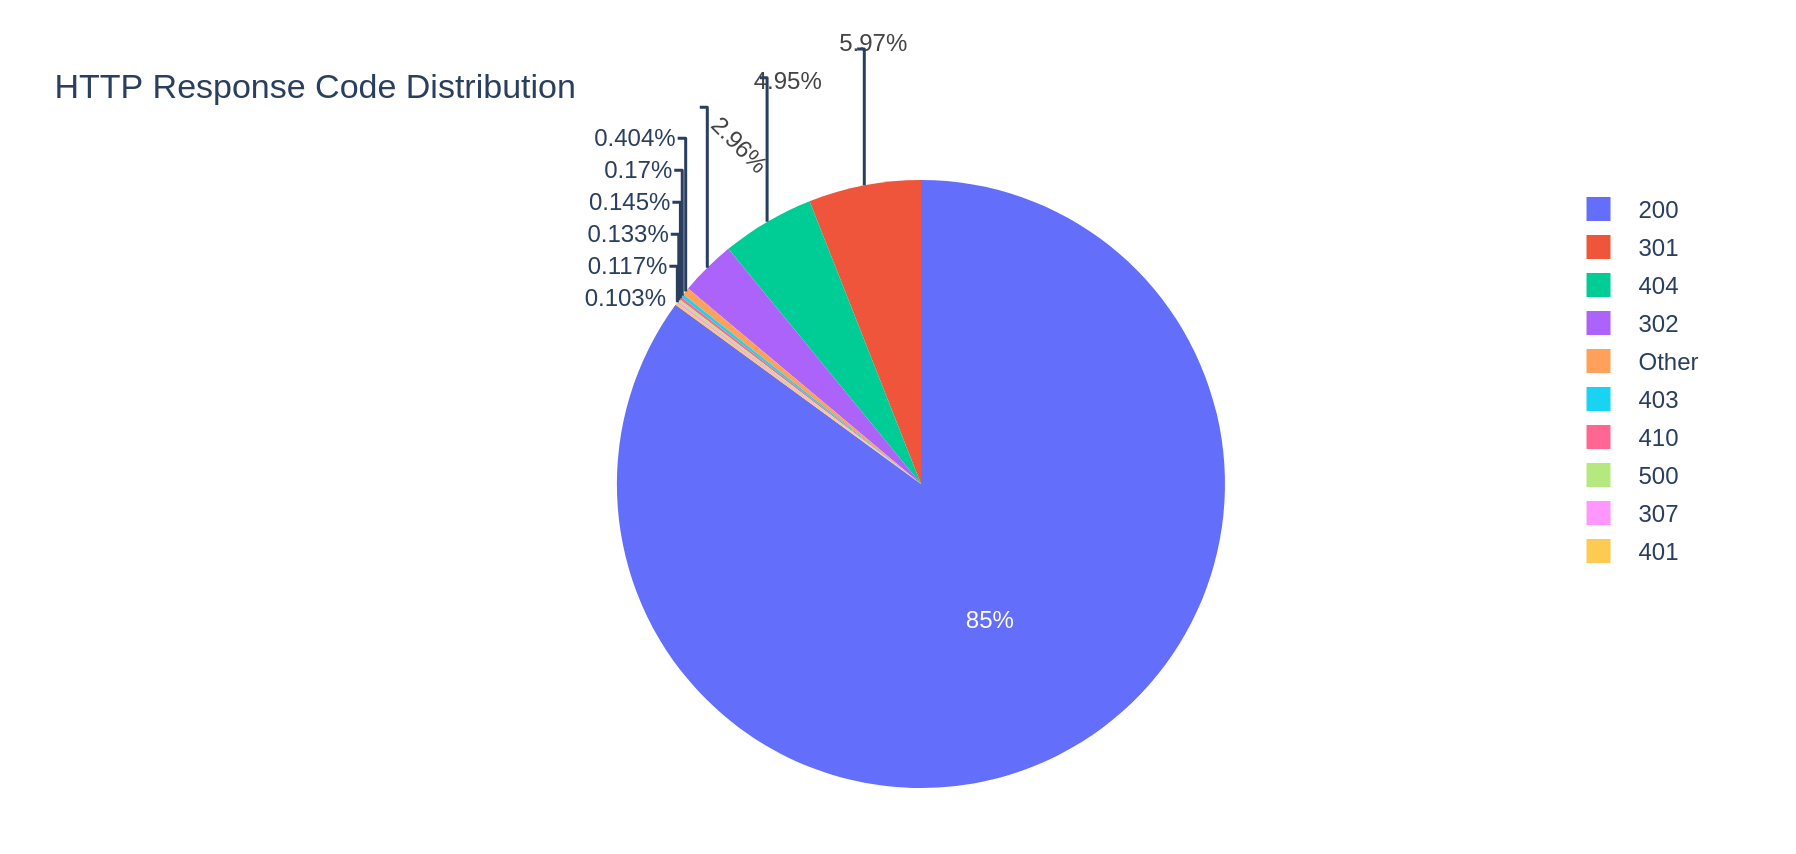
\includegraphics[width=\textwidth]{figures/charts/large/appendix/chart_source_response_code_pie.png}
    \caption{Response code distribution.}
    \label{fig:analysis-dataset-chart_source_response_code_pie}
\end{figure}

\Cref{fig:analysis-dataset-chart_source_charset_heatmap_response_code} compares charsets and response codes directly.
The heatmap displays a high frequency of status code occurrences per charset in yellow, with a low count shown in purple.
According to \ac{rfc} 7231, the \texttt{200} to \texttt{299} range is designated for successful responses, the \texttt{300} to \texttt{399} range for redirections, the \texttt{400} to \texttt{499} range for client errors, and the \texttt{500} to \texttt{599} range for server errors.

This chart also suffers from representation issues, such as with the \texttt{latin} charset, which is represented by only one website in our dataset.
For the \texttt{latin} charset, the \texttt{300} to \texttt{399} range shows up in bright yellow, as the single website returned a \texttt{302} response.
The chart is normalized by total charset count so that fields for charsets other than \texttt{utf-8} still exhibit color variation.

Incorrectly formatted charsets are prevalent, and 85\% of all responses have the \texttt{200} status code.
Due to these facts, additional comparisons among frequently occurring charsets would be necessary to identify patterns, such as whether certain charsets are more often associated with error pages than with successful responses.


\subsubsection{Analysis of aggregate data}
\label{sec:analysis-dataset-aggregate}

Now that we have established sufficient context to estimate the quality of our source data, we can shift our focus to analyses of global semantics.
More specifically, we will inspect web technology usage on both global and country-specific scales.
The graphs shown in this section are based on queries against the \texttt{fact\_website} table from the gold stage's \texttt{marts} namespace.

First, we visualize the mapping of \acp{cctld} to countries, which required assigning a matching ISO 3166 alpha-3 code to each \ac{uri}, as shown in \cref{lst:implementation-pipeline-visualization-chart}.
\Cref{fig:analysis-dataset-chart_fact_uri_choropleth} displays a choropleth map on which countries appear more yellow the more \acp{uri} with a matching \ac{cctld} they have, and more purple if they have fewer \acp{uri} with a matching \ac{cctld}.

Immediately, the country with the largest landmass, Russia, stands out in bright yellow.
There are approximately 326,177 websites with a \texttt{.ru} \ac{tld} in our dataset, accounting for 10.5\% of all websites with a \ac{cctld} and 4.4\% of all websites ingested overall.
Next, Germany, with its \ac{cctld} \texttt{.de}, is marked in light green as another country with a significant share of websites: approximately 287,434 websites, representing 9.2\% of the \ac{cctld} subset and 3.9\% of all ingested websites, are attributed to Germany.
Countries attributed with between 100,000 and 200,000 websites include the United Kingdom (159,216), Japan (154,911), Italy (140,071), France (132,077), Poland (124,659), Brazil (116,443), and the Netherlands (112,973).
Countries with between 50,000 and 100,000 websites include Australia (80,816), Czechia (77,221), Spain (69,634), Canada (68,759), China (57,013), and Ukraine (50,415).
All countries in Africa appear in purple, indicating that only a few websites are assigned to African \acp{cctld}.

\begin{figure}[H]
    \centering
    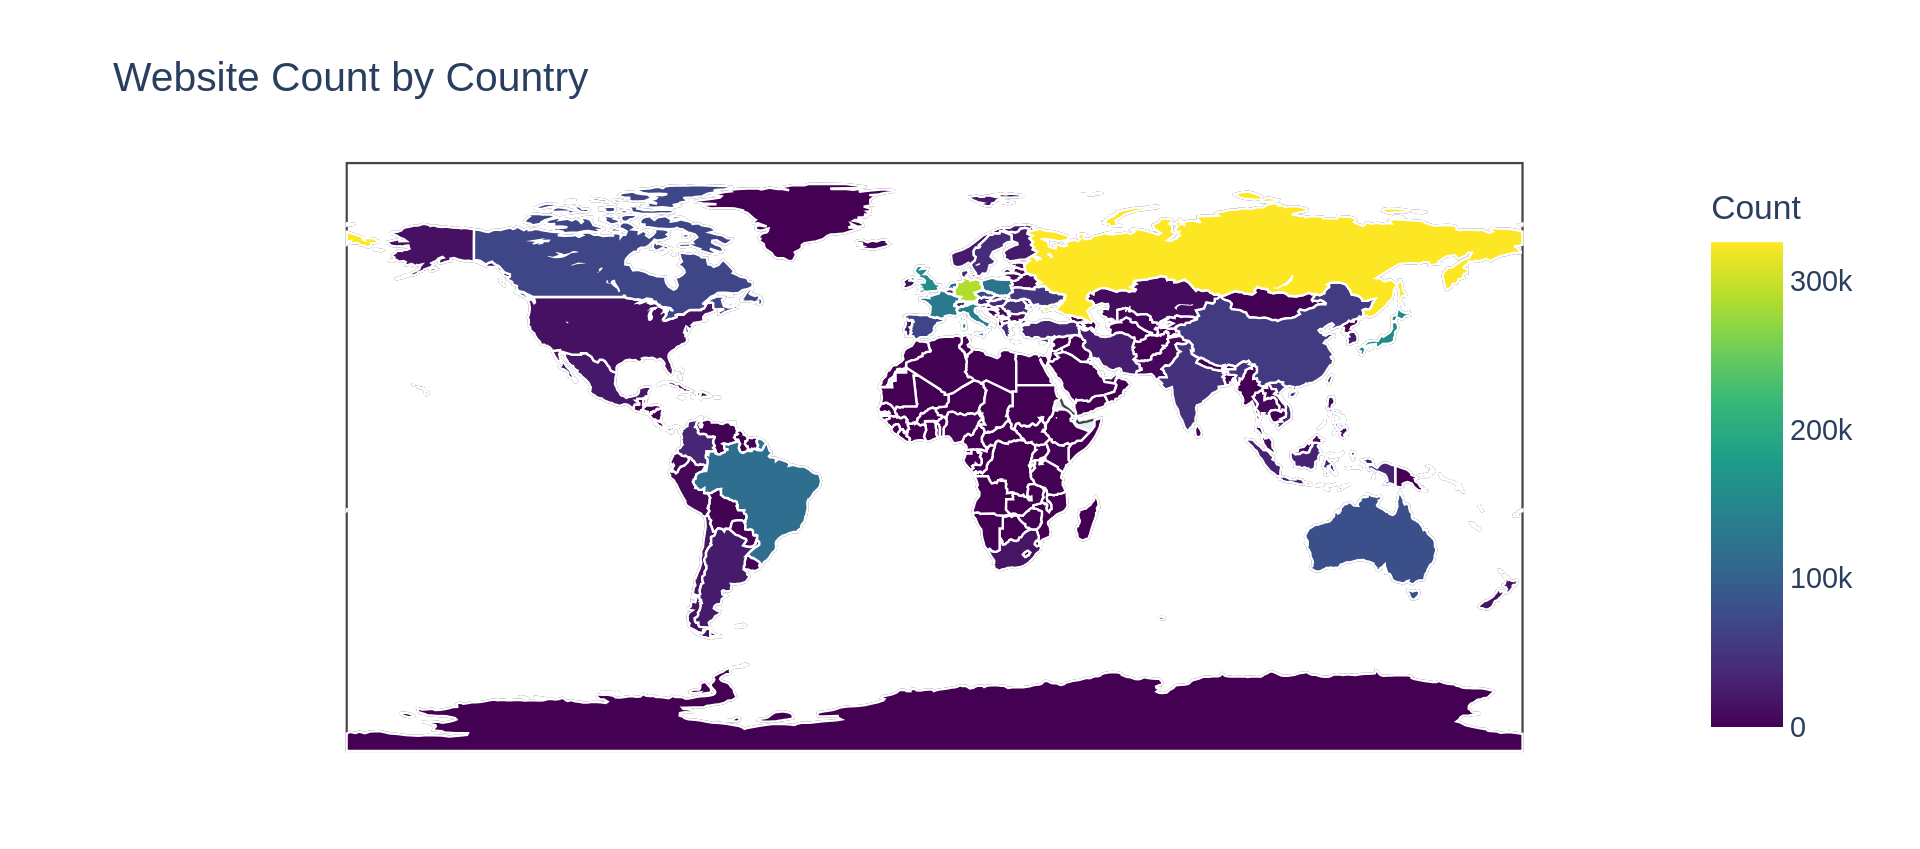
\includegraphics[width=\textwidth]{figures/charts/large/chart_fact_uri_choropleth.png}
    \caption{Total website count by country.}
    \label{fig:analysis-dataset-chart_fact_uri_choropleth}
\end{figure}

Comparing \cref{fig:analysis-dataset-chart_fact_uri_choropleth} with a choropleth map of world population in \cref{fig:analysis-dataset-population} reveals several differences.
The two most populous countries, India and China, each with over 1.4 billion people, rank far below Russia in website count within our dataset.
Although Russia has a relatively high population of 145 million, it is still only about one-tenth of the population of India or China.
Europe and South America display similar patterns on both maps.
In North America, however, the roles of Canada and the United States appear reversed: while the U.S. population (345 million) is nearly ten times that of Canada (40 million), Canada has about four times as many websites (60,000) as the U.S. (15,000) in our dataset.
Similarly, African countries exhibit much greater variation in population counts compared to their website counts~\cite{WPR2024}.

It is also important to note that \cref{fig:analysis-dataset-population} uses a different color scale, not only in terms of color range but also with an exponential increase in saturation, whereas \cref{fig:analysis-dataset-chart_fact_uri_choropleth} employs a continuous color scale.

\begin{figure}[H]
    \centering
    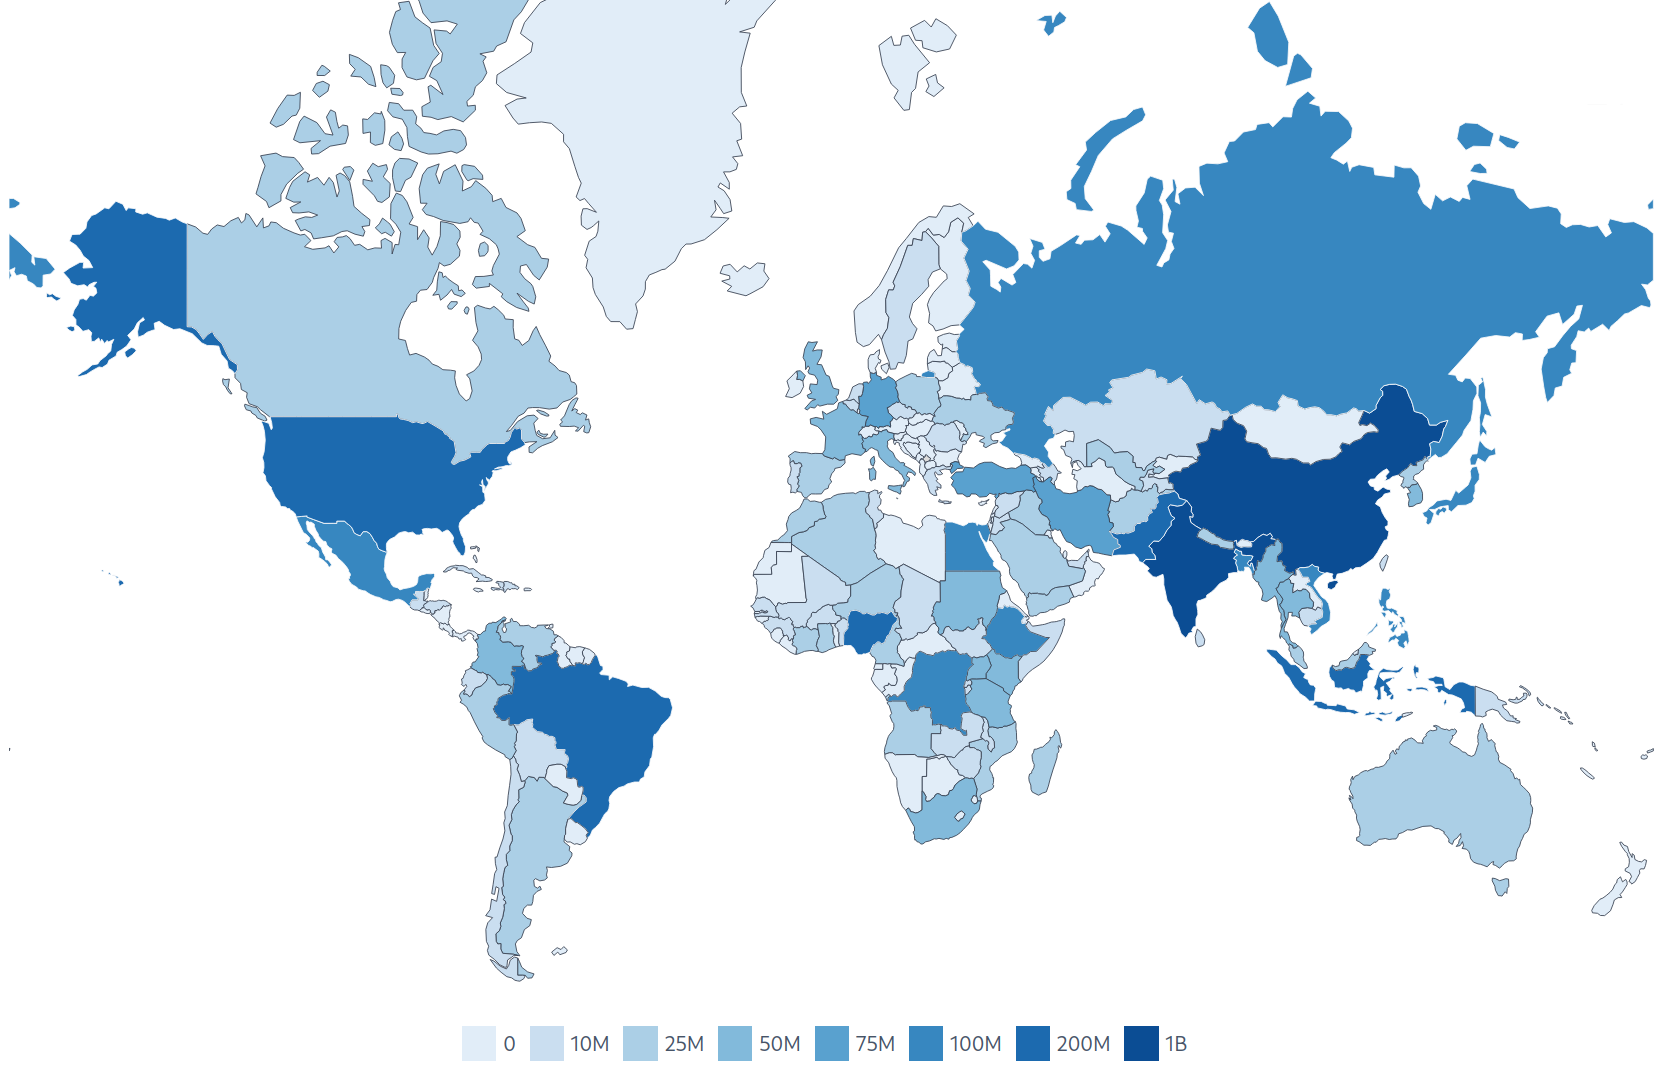
\includegraphics[width=0.6\textwidth]{figures/charts/population_choropleth.png}
    \caption{Total Population by Country, 2024~\cite{WPR2024}.}
    \label{fig:analysis-dataset-population}
\end{figure}

All 3,117,139 \ac{html} sources were pattern-matched using 422 \acp{regex} to determine indicators of specific web technology usage.
In total, 3,779 web technologies were sourced from Wappalyzer, of which 325 had defined \acp{regex} for matching on \ac{html} such as \texttt{\textless img[{\textasciicircum}>]+moodlelogo} for \href{https://moodle.de/}{\textit{Moodle}}.
Some web technology definitions had multiple \acp{regex} assigned.

The most frequently detected web technology across all \ac{html} sources is WordPress, identified in 924,000 \ac{html} sources, equivalent to 36.6\% of all web technology detections.
The second most frequently detected technology is \textit{Google Tag Manager}, with 552,000 detections, accounting for 21.9\% of all detections.
The remaining technologies in this ranking each have fewer than 90,000 detections: \textit{Gravatar} (89,000), \textit{YouTube} (89,000), and \textit{LiveInternet} (84,000).
Ten web technologies were detected on only one page, including \textit{SonarQube}, \textit{cPanel}, and \textit{Microsoft Publisher}.
\Cref{fig:analysis-dataset-chart_fact_web_technology_bar_top_10} shows the top 10 ranking web technology detections, and \cref{fig:analysis-dataset-chart_fact_web_technology_pie} represents similar information in a pie chart.

\begin{figure}[H]
    \centering
    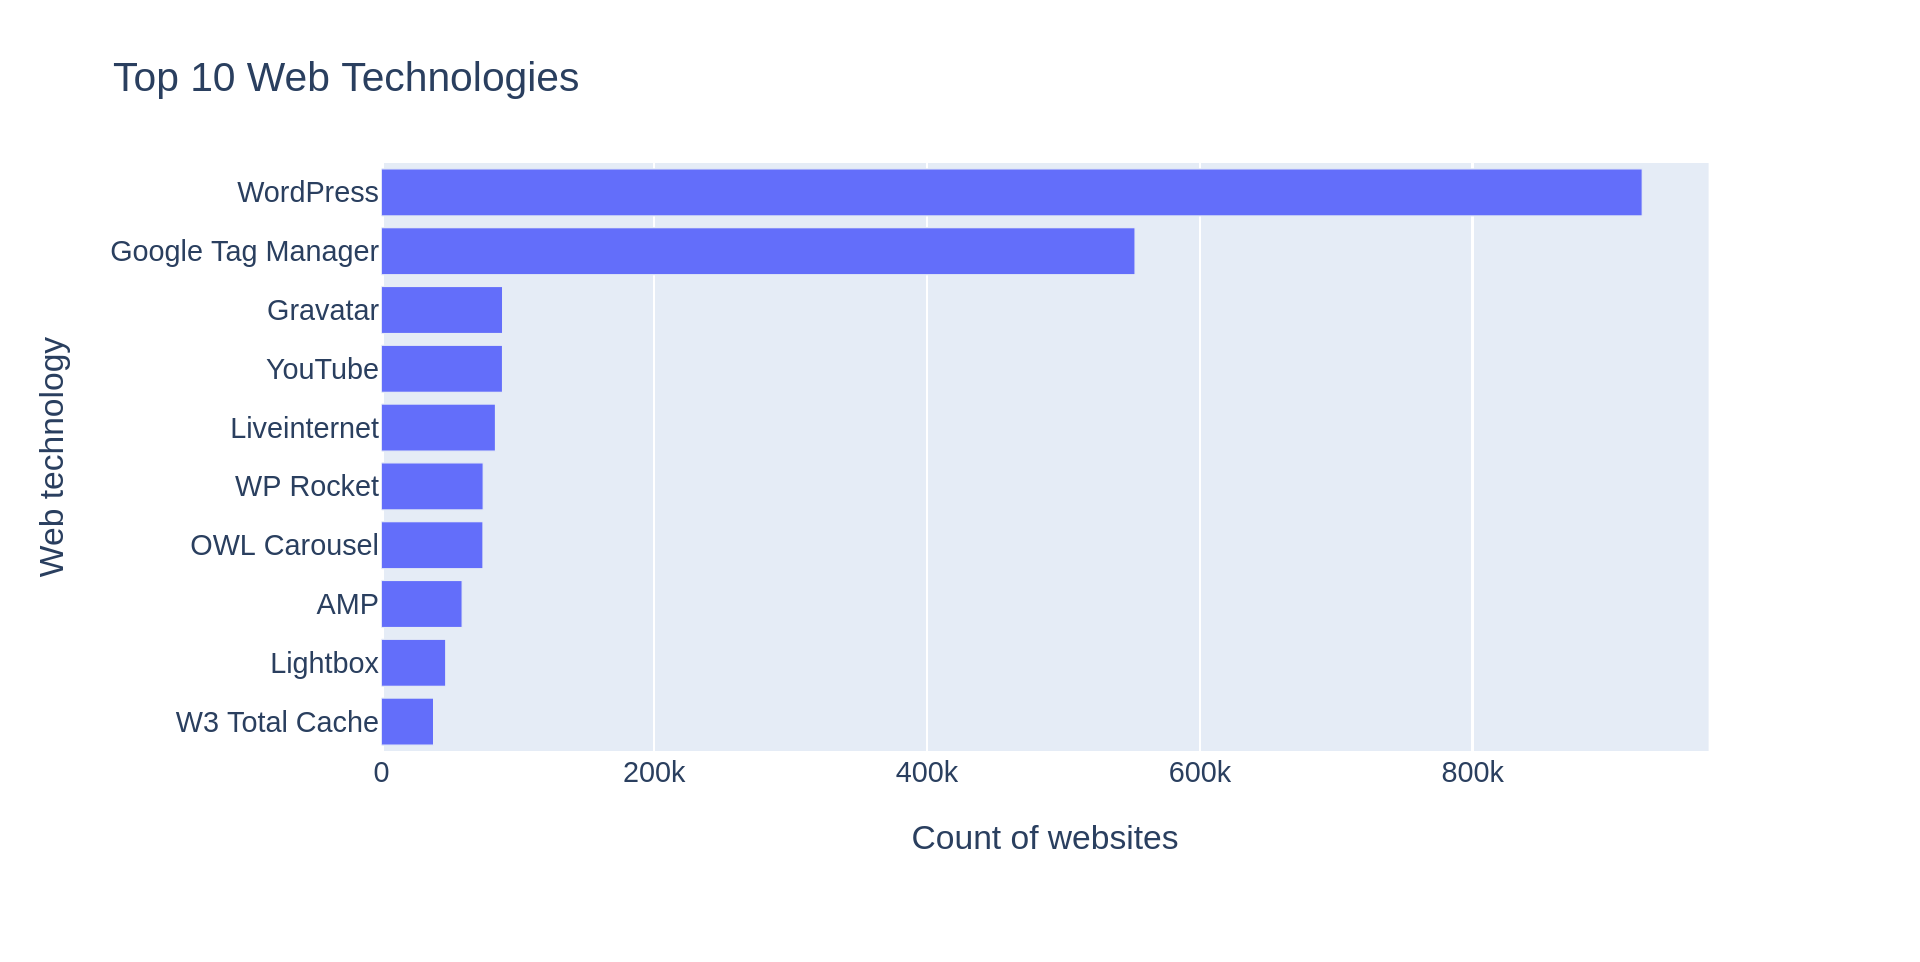
\includegraphics[width=\textwidth]{figures/charts/large/chart_fact_web_technology_bar_top_10.png}
    \caption{Top 10 web technologies found.}
    \label{fig:analysis-dataset-chart_fact_web_technology_bar_top_10}
\end{figure}

Next, we combine web technology detections with country information in \cref{fig:analysis-dataset-chart_fact_web_technology_choropleth_average}.
This choropleth map shows the average count of web technologies on websites for each country.
Due to the limited expressiveness of data from countries with relatively few attributed websites, we focus on the countries previously discussed for \cref{fig:analysis-dataset-chart_fact_uri_choropleth} and omit discussion of color variation in Africa.

The countries with the highest number of attributed websites all show similar averages of web technologies per website: United Kingdom (0.8), Japan (0.87), Italy (0.94), France (0.79), Poland (0.81), Brazil (0.95), and the Netherlands (0.97).
Notably, China's average web technology count per website is 0.19, which is significantly lower, especially given that China ranked 14th in our earlier analysis of website count by country.

Some regions with particularly high or low average web technology counts are often islands: Pitcairn (0.0), Nauru (0.0), Norfolk Island (0.01), Guinea-Bissau\footnote{Guinea-Bissau is not an island.} (1.91), Martinique (1.53), and Saint Kitts and Nevis (1.44).
Excluding countries with fewer than a thousand websites, the lowest average web technology counts were found in China (as noted), the Republic of Korea (0.43, 25k websites), and the Cocos (Keeling) Islands\footnote{Under the administration of Australia.} (0.43, 11k websites), while the highest were observed in the Dominican Republic (1.2, 2k websites), Israel (1.12, 15k websites), and North Macedonia (1.04, 3k websites).

\begin{figure}[H]
    \centering
    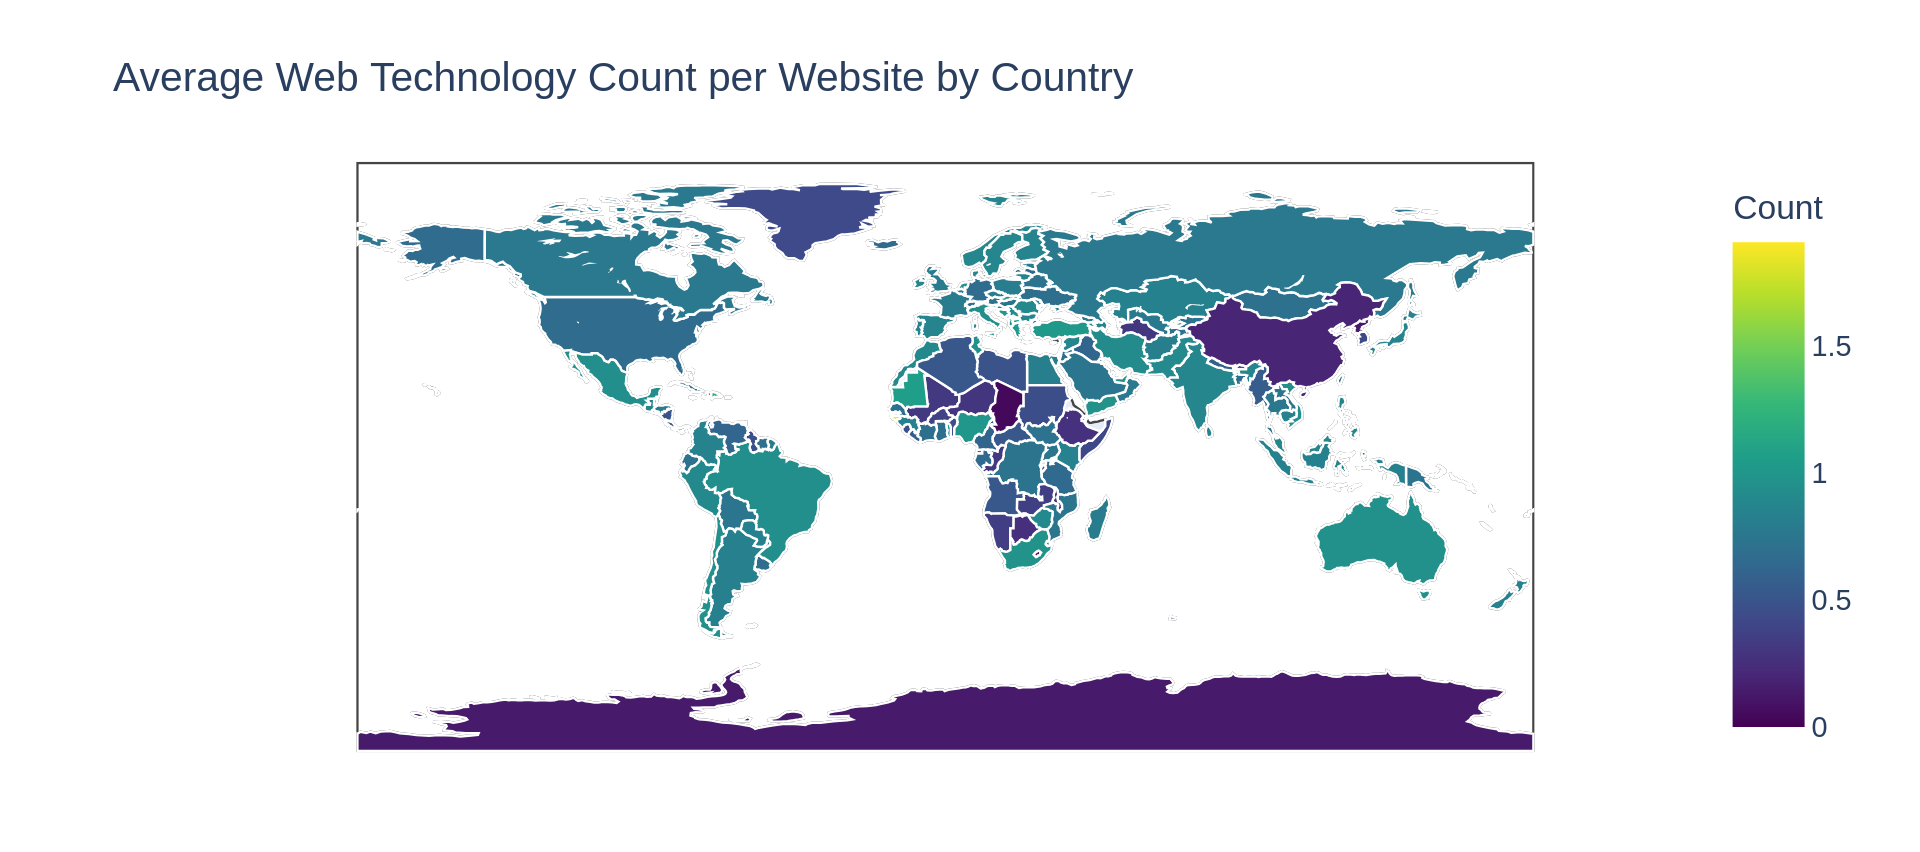
\includegraphics[width=\textwidth]{figures/charts/large/chart_fact_web_technology_choropleth_average.png}
    \caption{Average web technology count per website by country.}
    \label{fig:analysis-dataset-chart_fact_web_technology_choropleth_average}
\end{figure}

Similar to the average web technology count analysis, we can inspect the maximum web technology counts for each country, as visualized in \cref{fig:analysis-dataset-chart_fact_web_technology_choropleth_maximum}.
We keep this analysis brief for the same reason we avoided discussing countries with few attributed websites in depth: a single website with a high number of detected web technologies can make an entire country appear prominently in yellow.

For both Germany and Australia, there was at least one website with eight detected web technologies.
The maximum number of detected web technologies for Russia is seven, for China five, and for Brazil six.

\begin{figure}[H]
    \centering
    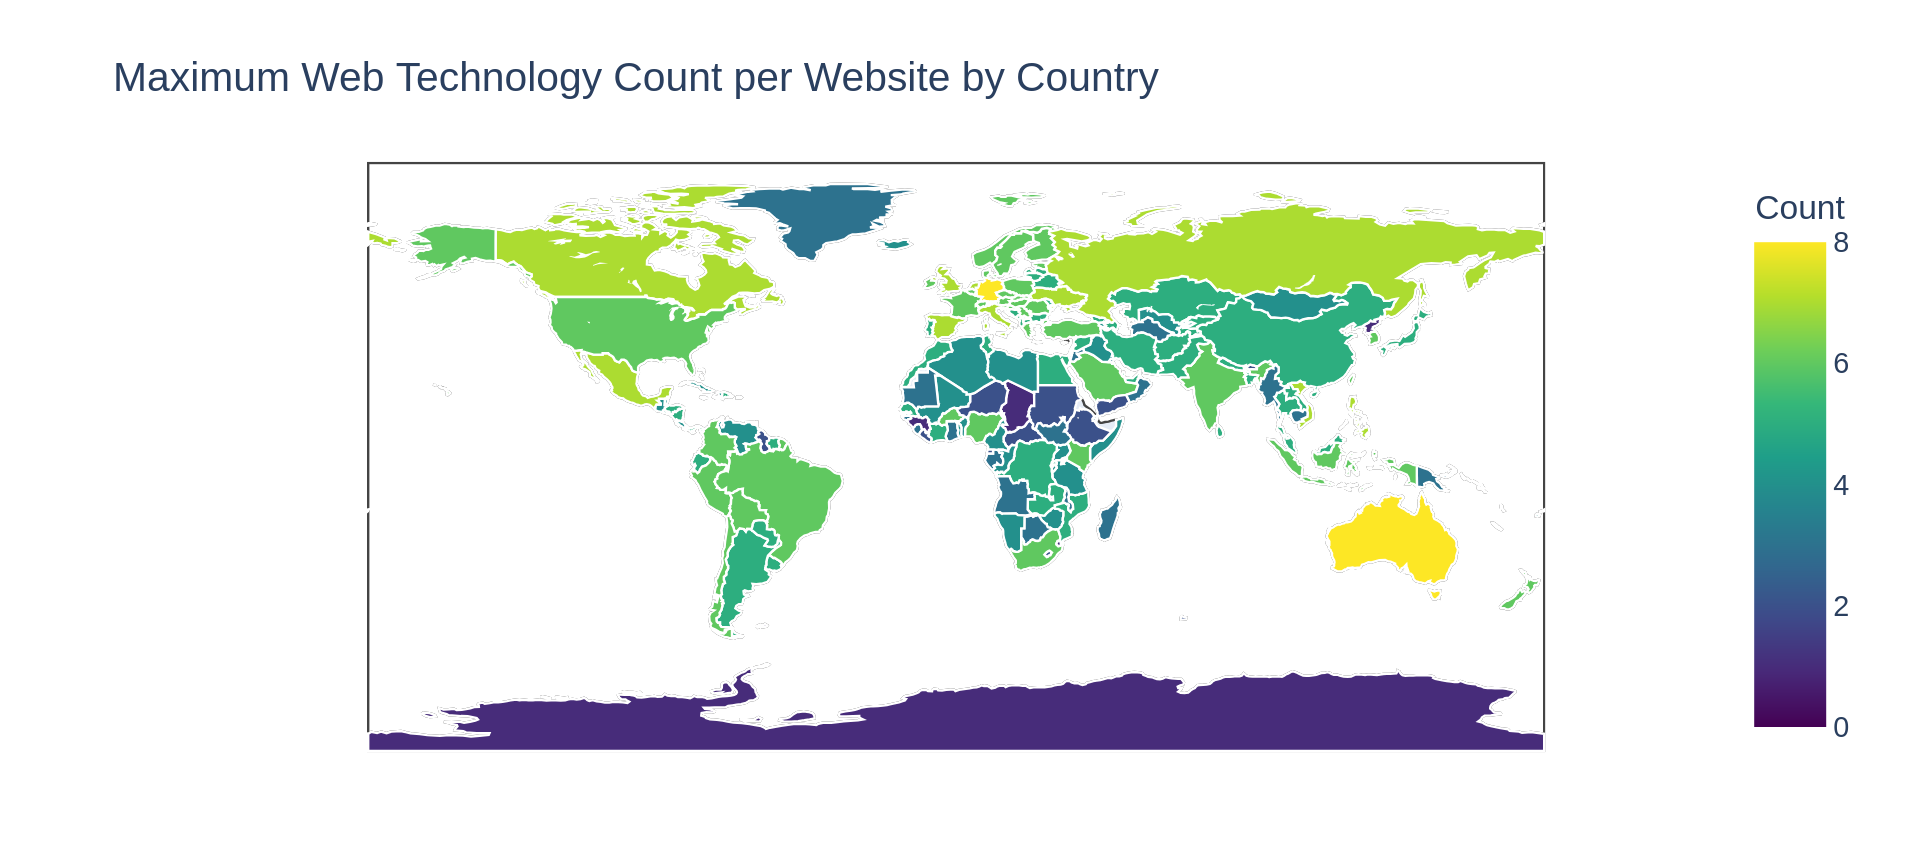
\includegraphics[width=\textwidth]{figures/charts/large/chart_fact_web_technology_choropleth_maximum.png}
    \caption{Maximum web technology count per website by country.}
    \label{fig:analysis-dataset-chart_fact_web_technology_choropleth_maximum}
\end{figure}

Whenever it seems worthwhile to explore specific differences between countries in more detail, we can generate a targeted graph using a simple function like the one shown in \cref{lst:implementation-pipeline-visualization-chart}.
\Cref{fig:analysis-dataset-chart_fact_web_technology_violin} presents a violin plot visualizing the distribution of web technology counts across web pages for the United States of America, Germany, and Japan.
The chart is normalized so that the highest web technology count equals one.

In the chart, the red area, representing Germany, extends furthest vertically at the upper end, indicating a high maximum web technology count for German websites.
At the lower end, the red area also stretches vertically, showing that many German pages have a low web technology count.
The green area, representing Japan, does not stretch as far vertically, either at the lower or upper end, suggesting fewer Japanese websites with very low or very high web technology counts compared to Germany.
However, the green area is horizontally wider in the mid-range of the y-axis, indicating that Japanese websites more commonly have a medium number of web technologies.
The blue area, representing the United States, is narrow and almost indistinguishable in the image but is more visible in the interactive \ac{html} version of the graph.
Websites from the United States follow the German pattern, with fewer websites having higher web technology counts, but overall with lower counts.

\begin{figure}[H]
    \centering
    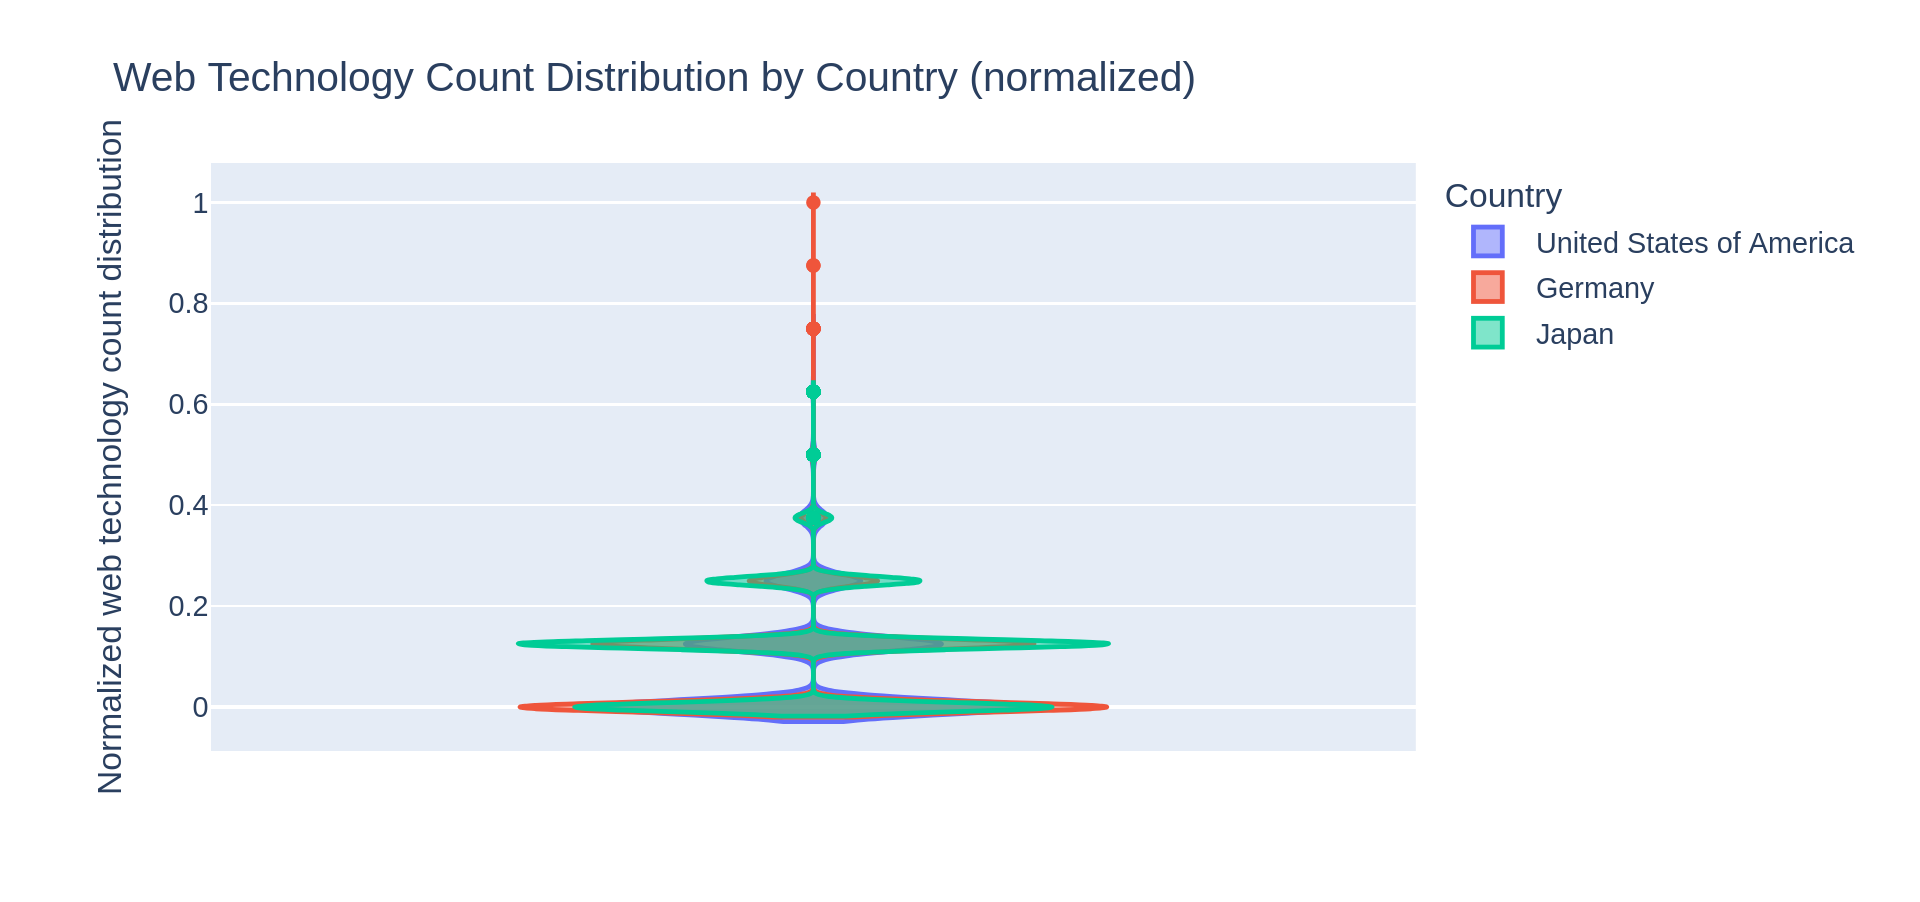
\includegraphics[width=\textwidth]{figures/charts/large/chart_fact_web_technology_violin.png}
    \caption{Distribution of web technology count by country.}
    \label{fig:analysis-dataset-chart_fact_web_technology_violin}
\end{figure}

Finally, \cref{fig:analysis-dataset-chart_fact_web_technology_heatmap_country} shows a heatmap of all web technologies across all countries.
Two main web technologies, WordPress and Google Tag Manager, are apparent due to the bright lines that span the primarily blue map.
Additionally, there is a less pronounced horizontal line with one very bright cell where Russia intersects with LiveInternet, a Russian web analytics service.
This chart highlights the importance of considering normalization for data visualization.

\Cref{fig:analysis-dataset-chart_fact_web_technology_heatmap_country_normalized} shows a version of the heatmap normalized for relative frequencies per country as well as per web technology.
In the normalized chart, many more bright cells are visible.
The alphabetical sorting of web technologies and country names results in an even distribution of highlighted fields.
Alternative sortings, such as by population, could reveal further insights.
One observation from this graph is that no single country uses the majority of web technologies, and no single web technology is used across most countries.
The majority of web technologies are embedded by only a few websites.


\newpage
\acresetall
\cleardoublepage
\section{Evaluation}
\label{sec:evaluation}

Now that we have run our Big Data pipeline to obtain the results shown in the preceding chapter, we will evaluate the answers to our research questions defined in \cref{sec:intro-research-question}.
We will also revisit the objectives of this thesis and discuss whether they have been met by our pipeline design.

\subsection{Research Questions}
\label{sec:evaluation-rq}

The answers to our research questions were partly derived from the literature review conducted in \cref{sec:related-work} and from the insights gained by implementing our design proposal.

\begin{enumerate}
    \item[] \textbf{\Cref{rq:0} Can we test or refute hypotheses on global variations in website code?}

    The pipeline designed in this work is capable of processing any data that allows hypotheses to be tested or refuted.
    The capabilities of this pipeline are not limited to variation detection, the domain of websites, or even code in general.
    Our goal to create a modular pipeline for a specific use case, paired with research on modern Big Data pipelines, led us to design a system from the perspective of a data engineer, rather than a web developer.
    We view this as a significantly beneficial architectural decision, as this thesis was primarily intended to lay a foundation for future researchers and thus should not be unnecessarily constrained.

    \item[] \textbf{\Cref{rq:1} What influence does culture have on code?}

    Our literature review identified scientific evidence for cultural influences on behavior, notably Hofstede's cultural dimension theory.
    Sources such as Shah and Harrold provided specific observations on cultural differences in development practices across the globe.
    For instance, Japanese culture is said to have a high \ac{lto} and a tendency to reject expatriate leaders with short-term success orientation~\cite{CFG2024, Marshall}.
    Shah and Harrold observed that a Japanese development team ensured high code quality through meticulous testing, while a U.S. development team placed less emphasis on testing functionality outside core features.

    \item[] \textbf{\Cref{rq:2} Which global variations in code have been researched before?}

    A review of related work revealed no general analysis of code variations at a global scale.
    However, code variations have been studied on a smaller scale for specific use cases, such as code authorship attribution.
    For example, Caliskan-Islam et al. (2015) demonstrated that even with over 1,000 developers, individual code styles could remain distinctive enough to allow accurate author identification~\cite{CaliskanIslam2015}.
    Code variation detection is also commonly used in plagiarism detection.

    \begin{enumerate}
        \item[] \textbf{\Cref{rq:21} Which specific feature patterns in website code can be identified and analyzed for global variations?}

        In this thesis, we demonstrated the detection of web technologies through \ac{regex} pattern matching on over seven million \ac{html} documents.
        As mentioned in the evaluation for \Cref{rq:0} above, our pipeline is not limited to specific types of analysis; any hypothesis on feature patterns for which a fitting dataset is available can be analyzed.

        A set of feature patterns for web design analysis is provided by Alexander et al. (2016)~\cite{Alexander2016}.
        They analyze layout (page structure), navigation (menu structure), links, multimedia (interaction possibilities), visual representation (use of images), color, and text of 460 websites.

        Various literature addresses specific feature patterns on smaller scales.
        We found little information on broader patterns at larger scales and thus consider further research on this topic to be worthwhile.

        \medskip
        \item[] \textbf{\Cref{rq:22} Which statistical methods and algorithms are effective in detecting global variations in website code?}

        As we found no technical limitations to the types of data our pipeline can process and limited quantitative research at a global scale, the effectiveness of statistical methods and algorithms for variation detection in code depends on the use case.
        For example, Alexander et al. used the Chi-square method for feature comparisons.
        Anomaly detection is often performed using clustering algorithms such as \textit{k-means} and \textit{DBSCAN}~\cite{Chen2014, Mussabayev2023}.
    \end{enumerate}

    \item[] \textbf{\Cref{rq:3} Which data sources can be used to yield valuable insights?}

    Our pipeline design allows for any data to be ingested as long as an ingestion method can be defined in Python.
    In the context of website data, we note that large crawling datasets are publicly available, allowing general analysis without the complexities of setting up a custom crawler.

    \begin{enumerate}
        \item[] \textbf{\Cref{rq:31} Which datasets include the feature patterns under study and are publicly available?}

        The two primary datasets that, by being large and containing website data, fit the goal of this thesis are the Common Crawl and HTTP Archive datasets.
        The Common Crawl dataset is stored by \ac{aws}, and the HTTP Archive dataset by \ac{gcp}.
        The Common Crawl dataset is accessible via \ac{http} without authentication, though rate limiting may apply.
        The HTTP Archive dataset is tailored toward performance metrics, while the Common Crawl dataset is not.
        The file format used by Common Crawl is the \ac{warc} file format, while the HTTP Archive uses the \ac{har} file format.
        The Common Crawl dataset is considerably larger than the HTTP Archive dataset, with around 250 billion and 15 million websites included, respectively.

        \medskip
        \item[] \textbf{\Cref{rq:32} In which ways can useful datasets be sourced independently?}

        Depending on the required level of abstraction, e.g., to satisfy security measures such as those provided by services like Cloudflare, different tools are available for web data crawling.
        Apache Nutch is a robust solution for distributed crawling, as demonstrated by Common Crawl's use of it.
        If proper browser emulation is needed, a tool like Selenium should be chosen instead.
        It is essential to avoid excessive load on source servers to prevent timeouts or blacklisting.
    \end{enumerate}

    \item[] \textbf{\Cref{rq:4} What is the current state of Big Data and data engineering?}

    The exponential increase in data storage is a phenomenon of the 21st century, and the term ``Big Data'' emerged alongside it.
    While the concept of data warehousing can apply to smaller-scale data, data lakes were designed to store data from various sources at large scale.
    As data volumes continue to grow with no end in sight, data engineers have become increasingly important.

    \begin{enumerate}
        \item[] \textbf{\Cref{rq:41} What constitutes a modern Big Data pipeline design?}

        A recent development, the Lakehouse concept, aims to unify data lakes and data warehouses.
        This unification was driven by a decrease in storage costs, especially for S3-compatible object storage.

        We argue that a modern Big Data pipeline should not leave any compute resources unused and should focus on full resource utilization rather than premature optimizations, especially when run in a distributed system.
        The context of application should also be considered carefully to allow deliberate decisions for or against stream-based tooling in real-time applications.

        \medskip
        \item[] \textbf{\Cref{rq:42} How can the effectiveness and accuracy of the pipeline be benchmarked?}

        Ensuring the quality of ingested data is crucial, as processing poor-quality data can impair result accuracy.
        For the Common Crawl dataset, the publisher provides dataset statistics, which can be compared against those from a fetched subset to identify potential issues.
        This was especially useful in our analysis of global web technology usage, as even our small subset of the most recent Common Crawl dataset exhibited characteristics similar to those reported for the entire dataset.
        We therefore believe that our analysis is based on a representative subset of Common Crawl's full dataset.

        Timing measurements allowed us to adjust the pipeline's performance and identify issues with the tools used.
        Standardized benchmarks like \textit{TPC-H} and \textit{TPC-DS} could be run to accurately compare our pipeline's design to similar systems~\cite{Bajaber2020, Ivanov2020}.
        However, we did not conduct such benchmarks, as this type of performance evaluation is outside the scope of this thesis.
    \end{enumerate}
\end{enumerate}

\subsection{Objectives}
\label{sec:evaluation-objectives}

The technical objectives defined in \cref{sec:intro-objectives} guided our pipeline design and implementation.
We revisit these objectives now to evaluate whether they have been reached as intended.

\begin{enumerate}
    \item \textbf{Design and implement a scalable data pipeline}

    In \cref{sec:design}, we proposed a combination of several tools and technologies that together form a modular Big Data pipeline.
    The pipeline is scalable, as both the number of compute workers and the size of storage volumes can be adjusted variably.
    The implementation outlined in \cref{sec:implementation} produced a system that was capable of generating the results showcased in \cref{sec:analysis}, fulfilling all architectural requirements.

    One pipeline component, dbt, was found to suffer from minor performance issues.
    The inclusion of dbt in the proposed pipeline stack is optional, though, and can be substituted by raw \ac{sql} strings defined in Python.

    In addition to flexibility, the pipeline's modularity implies some maintenance complexity.
    All running containers must include compatible versions of tooling such as Spark, Iceberg, as well as Python and Java.
    Updates to the container images are currently not provided by a third party, so these must be managed by a future pipeline maintainer for now.

    We configured the Spark workers to install a necessary dependency for our workloads at boot time.
    This customization should be avoided for a clean separation of concerns.
    Instead, custom functions to run on Spark workers should be encoded as \acp{udf}.

    \item \textbf{Identify and quantify global variations in website code}

    In \cref{sec:analysis-dataset}, we analyzed source data and combined data by examining web technology usage across nations.
    We thus succeeded in identifying and quantifying global variations in website code, although more diverse analyses would be desirable.
    Such further analyses are intentionally left for future researchers, as the scope of this thesis is the design, implementation, and exemplary use of a Big Data pipeline.

    \item \textbf{Evaluate the qualitative performance of the data pipeline}

    The statistics published by Common Crawl, with certain metrics mentioned in \cref{sec:related-work-big-data-datasets}, allow us to assess the data quality of our ingestion process.
    The full Common Crawl dataset, from which we ingested a subset, contains 43.22\% of \acp{cctld} and 4.6\% of \texttt{.ru} \acp{cctld}, whereas our subset contains 41.9\% of \acp{cctld} and 4.4\% of \texttt{.ru} \acp{cctld}.
    In the full dataset, the predominant charset is \texttt{UTF-8} with a share of 93.3\%, and in our subset, \texttt{UTF-8} is also the most frequent charset, with 87.6\%.
    This leads us to believe that the quality of the ingested data subset is fairly representative.

    \item \textbf{Formalize a data ingestion module definition}

    Following our choice of Iceberg as a unified yet open storage format, Spark as the compute engine, and Python as a widely supported and tool-compatible programming language, we revisit an idea introduced as part of the intuitive approach in \cref{sec:design-prerequisites-intuitive-approach}.
    The concept was to construct the pipeline from distinct services, each potentially using a different programming language and storage solution.
    The hypothesis was that high pipeline performance could be achieved by selecting the most efficient execution engine and storage system for each type of computation.
    For example, regex matching could theoretically be faster in a specific programming language, which may differ from the language best suited for numerical operations.
    Similarly, binary output from one transformation step might be stored most efficiently in one storage solution, while scalar values could be more efficiently stored elsewhere.

    This approach to service architecture could theoretically enable the most optimized implementation of a data pipeline.
    However, it is important to note that data written by one service would need to be read by another, and there is no guarantee that the output format of one service is ideally suited as input for another.
    Moreover, service requirements may change over time, potentially negating any performance gains previously achieved.

    Evaluating the most efficient solution for each specific case would be disproportionately time-consuming.
    Additionally, the implicit optimization required for unique combinations of pipeline services is unlikely to justify the added complexity.
    For these reasons, we will not define an interoperability interface for a highly detailed service architecture and will instead leverage the foundational tool combination outlined previously.
\end{enumerate}


\newpage
\acresetall
\cleardoublepage
\section{Future Work}
\label{sec:future_work}

This thesis aims to serve as a foundation for plentiful future research endeavors.
The pipeline definition designed in this thesis was created with extensibility and modularity in mind.
Therefore, various extensions, optimizations, and even replacements of pipeline components can be made.
The following sections provide inspirations for such future work.

\subsection{Extensions}
\label{sec:future-work-extensions}

Due to the full flexibility in data sources to ingest and in transformation functions to code, there is significant freedom in developing additional modules.
Code-level analysis could be performed on links included in a page's \ac{html}, on \ac{css} complexity, on code formatting, or on variable naming conventions.
The existence or frequency of comments in code, the use of code minification, or \ac{nlp} analysis could also help identify culture-specific developer habits.
Additionally, page-level metrics, such as sitemaps of a website, could be inspected.
Network information, such as \ac{ip} addresses of servers distributing website content, could also be incorporated.
As illustrated by the networking example, entirely new data dimensions can be incorporated beyond the topics discussed in this thesis.

Beyond extensions to the pipeline's workflow, quality assurance could also be improved.
For example, additional data tests could be defined in dbt, and unit tests for Python functions could be added.

Further work could also focus on handling data updates, for instance, by implementing versioning strategies tailored to specific use cases.
Additionally, Iceberg's data snapshot, branching, and tagging functionalities could be made more accessible through utility functions.
The same applies to data maintenance tasks such as snapshot expiry, deletion of orphan files, and file compaction.

In recent years, many data engineering efforts have aimed to pave the way for \ac{ml} applications.
\textbf{Mangaonkar and Penikalapati}, for example, demonstrated how data pipelines' monitoring and reliability could be enhanced through \acp{llm}~\cite{Mangaonkar2024}.
Spark has a built-in \ac{ml} library named \textit{MLlib} that should already cover many common use cases.


\subsection{Optimizations}
\label{sec:future-work-optimizations}

As the ingestion of large amounts of data took by far the most time, as shown in \cref{tab:analysis-dataset-asset-times}, further research could focus on improving ingestion speeds for Iceberg.
A general comparison of distributed ingestion and computation speeds between Spark and other solutions, such as the \ac{olap} \acp{dbms} mentioned in \cref{sec:design-databases}, could be insightful, especially when considering parallel writes to the same table in a distributed architecture.
Significant reductions in ingestion durations could likely be achieved by using \href{https://py.iceberg.apache.org/}{\textit{PyIceberg}}, which avoids the detour through Spark, thereby saving on network transfers and marshalling overhead.

The combination of Spark and Iceberg should support parallel writes to different partitions of a single table, suggesting that strategies for optimal partitioning and write task distribution among workers could be developed.
A potentially helpful partitioning scheme could draw inspiration from the Internet Archive's \href{http://crawler.archive.org/articles/user_manual/glossary.html#surt}{\ac{surt}} scheme, which reverses the domain parts of a \ac{uri} to more closely resemble the \ac{dns} hierarchy when read from left to right.
In simple terms, this scheme allows for more intuitive sorting of \acp{uri} as the \ac{tld} appears first, followed by the second-level domain and subdomains.
Partitioning inspired by \ac{surt} allows for more nested partitions; a simpler variant could involve partitioning by \ac{tld} only.

Reliability optimizations for downloads from Common Crawl's data server have already been initiated through the exponential backoff decorator in \cref{lst:dagster-source-common-crawl-fetch}, but \ac{aws}'s \texttt{503} ``slow down'' \ac{http} response codes still occur frequently enough to cause long-running ingestion tasks to fail.
With the asynchronous nature of source file iteration, it is challenging to determine which of the 90,000 source files in each monthly Common Crawl dataset have already been ingested when an ingestion run is aborted.
Either a refined retry mechanism could increase resiliency in the face of network issues, or, ideally, the ingestion algorithm could be extended to include metadata tracking to log the dataset parts that have already been processed.

Another tool that could benefit from increased reliability is the \texttt{rest} pod currently operating in the pipeline.
At present, the \texttt{rest} pod is stateful and loses its catalog data\footnote{The \ac{rest} catalog mainly stores information on which tables exist and in which namespace they reside.} when stopped, for instance, if Kubernetes reschedules the \texttt{rest} pod to a different node.
It turns out that the \texttt{rest} pod is designed to store its catalog data in-memory, but due to a bug, it persists the catalog data as a file~\cite{Kolter2023}.
This flaw can be exploited to our advantage by mounting a volume as the file's parent directory, allowing this storage to persist across restarts.
The catalog's SQLite file is stored as \texttt{/tmp/iceberg\_rest\_mode=memory} (sic!) by default, but this location can be configured through the \texttt{CATALOG\_URI} environment variable.

There is ongoing work on an official Iceberg \ac{rest} catalog Dockerfile, which addresses the incorrect file creation issue~\cite{Bhat2024}.
When switching to the official Iceberg \ac{rest} container image in the future, the \texttt{CATALOG\_URI} will need to be set to ensure data persistency.

The Dockerfile provided in \cref{lst:appendix-listings-dockerfile} currently includes the code location for Dagster, Dagster's web server, and Dagster's daemon.
In an optimal deployment, these three components would be deployed separately.

Furthermore, the pipeline's dashboard is currently accessible to anyone on the internet as access authentication has not yet been implemented for this service.
The MinIO \ac{gui} is credential-protected as defined in \cref{lst:minio-compose}, and the Spark driver as well as the Chart web server are read-only, so they could theoretically remain as they are.

Currently, a single Dagster asset generates all charts as outlined in \cref{sec:implementation-pipeline-visualization}.
An improvement could involve having each table-filling asset generate its own graphs and link them in the asset's build metadata.

Finally, node affinity in Kubernetes could be improved.
The current deployment starts a specific number of Spark workers, one fewer than the number of nodes available in the Kubernetes cluster, as noted in \cref{sec:implementation-deployment}.
The idea behind this setup is to leave one node for the Spark master and to use the full capacity of all other nodes.
However, no mechanism is yet defined to ensure each node is utilized effectively and that one node is exclusively reserved for the Spark master.
Such a concept could be established if the pipelines designed in this thesis are used at scale.


\subsection{Replacements}
\label{sec:future-work-replacements}

The pipeline system's design is modular in the sense that individual parts can be substituted by other solutions within the same category.
For example, if requirements arise that make support for streaming necessary -- along with all conditions such an orientation would entail (discussed in \cref{sec:related-work-big-data}) -- Spark could be replaced by Flink.
Also refer to the \href{https://www.databricks.com/glossary/lambda-architecture}{\textit{Lambda Architecture}}, which outlines how to run batch and streaming processing in parallel, or to the \textit{Kappa Architecture}, a one-stream-fits-all iteration on the Lambda Architecture~\cite{Marz2011, Kreps2014}.

If self-hosted storage needs to be migrated to a cloud provider, the de-facto standard S3 allows this transition to happen comfortably.
For Iceberg, there are alternatives like Hudi and Delta Lake.
These alternatives can already be used in unison through XTable or Delta Lake UniForm.

Instead of the block storage abstraction provided by Longhorn, \ac{hdfs} could be evaluated to determine if it offers increased performance due to higher data locality.
This evaluation is especially useful if the pipeline is deployed on a cluster of machines with high network latency, i.e., geographically distant nodes.

The tool dbt can be removed completely if its assistance in structuring transformations is considered too complex, particularly if the pipeline is executed as individual instances rather than a centrally hosted pipeline shared by multiple users.
The \ac{sql} statement templating in dbt can be replaced by simple \ac{sql} strings in Python.

If Python is not considered the optimal programming language for the task, the \href{https://beam.apache.org/}{\textit{Apache Beam}} model allows pipelines to be defined in other languages such as Java, Go, TypeScript, and Scala.
Finally, if the modularity offered by the pipeline design in this thesis incurs too much maintenance effort, it is always possible to revert to an \ac{olap} \ac{dbms} like ClickHouse.


\newpage
\acresetall
\cleardoublepage
\section{Conclusion}
\label{section:conclusion}
%
% interessanter Einstieg
%
% Zusammenfassung der Arbeit
%
% Wichtigste Ergebnisse & Research Questions Beantwortung
% RQ 1
%
% RQ 1 Antwort
%
% RQ 2
%
% RQ 2 Antwort
%
% Forschungsstand und Ausblick
\lipsum


\schlussmatter
\newpage
\addcontentsline{toc}{section}{References}
\printbibliography

\newpage
\acresetall
\cleardoublepage
\renewcommand{\thefigure}{A\arabic{figure}}
\renewcommand{\thelisting}{A\arabic{listing}}
\renewcommand{\thetable}{A\arabic{table}}
\appendix

\section{Cultural Dimension Comparison: Germany and Japan}
\label{sec:appendix-country-comparison-tool-descriptions}

The following paragraphs are excerpts from the Country Comparison tool, visualized in \cref{fig:country-comparison}.

\begin{enumerate}
%     \item \ac{pdi}
%     \begin{itemize}
%         \item \textbf{Germany}
%         Highly decentralised and supported by a strong middle class, Germany is not surprisingly among the lower power distant countries (score 35).
%         Co-determination rights are comparatively extensive and have to be taken into account by the management.
%         A direct and participative communication and meeting style is common, control is disliked and leadership is challenged to show expertise and best accepted when it's based on it.
% % old dependency versions in Japan
%         \item \textbf{Japan}
%         At an intermediate score of 54, Japan is a borderline hierarchical society.
%         Yes, Japanese are always conscious of their hierarchical position in any social setting and act accordingly.
%         However, it is not as hierarchical as most of the other Asian cultures.
%         Some foreigners experience Japan as extremely hierarchical because of their business experience of painstakingly slow decision making process: all the decisions must be confirmed by each hierarchical layer and finally by the top management in Tokyo.
%         Paradoxically, the exact example of their slow decision making process shows that in Japanese society there is no one top guy who can take decision like in more hierarchical societies.
%         Another example of not so high Power Distance is that Japan has always been a meritocratic society.
%         There is a strong notion in the Japanese education system that everybody is born equal and anyone can get ahead and become anything if he (yes, it is still he) works hard enough.
%     \end{itemize}

    \item \ac{idv}
    \begin{itemize}
        \item \textbf{Germany}
        The German society is a truly Individualist one (79).
        Small families with a focus on the parent-children relationship rather than aunts and uncles are most common.
        There is a strong belief in the ideal of self-actualization.
        Loyalty is based on personal preferences for people as well as a sense of duty and responsibility.
        This is defined by the contract between the employer and the employee.
        Communication is among the most direct in the world following the ideal to be “honest, even if it hurts” – and by this giving the counterpart a fair chance to learn from mistakes.

        \item \textbf{Japan}
        Japan scores 62 on the Individualism dimension.
        Japanese society shows the characteristics of an individualistic society.
        Japanese society does not have an extended family system like China and Korea.
        Japan has been a paternalistic society and the family name and asset was inherited from the father to the eldest son.
        The younger siblings had to leave home and make their living with their core families.
        Japanese are famous for their loyalty to their companies, which people have chosen for themselves, which is an Individualist thing to do.
        You could say that the Japanese in-group is situational.
        Japanese are more private and reserved than most other Asians.
    \end{itemize}

    \item \ac{mas}
    \begin{itemize}
        \item \textbf{Germany}
        With a score of 66 Germany is considered a Decisive society.
        Performance is highly valued and early required as the school system separates children into different types of schools at the age of ten.
        People rather “live in order to work” and draw a lot of self-esteem from their tasks.
        Managers are expected to be decisive and assertive.
        Status is often shown, especially by cars, watches, and technical devices.

        \item \textbf{Japan}
        At 95, Japan is one of the most Decisive societies in the world.
        However, in combination with their mild collectivism, you do not see assertive and competitive individual behaviors which we often associate with a Decisive culture.
        What you see is severe competition between groups.
        From a very young age at kindergartens, children learn to compete on sports day for their groups (traditionally red team against white team).
        In corporate Japan, you see that employees are most motivated when they are fighting in a winning team against their competitors.
        What you also see as an expression of Decisiveness in Japan is the drive for excellence and perfection in their material production (monodukuri) and in material services (hotels and restaurants) and presentation (gift wrapping and food presentation) in every aspect of life.
        Notorious Japanese workaholism is another expression of their Decisiveness.
        It is still hard for women to climb up the corporate ladders in Japan with their Decisive norm of hard and long working hours.
    \end{itemize}

    \item \ac{uai}
    \begin{itemize}
        \item \textbf{Germany}
        Germany is among the uncertainty avoidant countries (65); the score is on the high end, so there is a slight preference for Uncertainty Avoidance.
        In line with the philosophical heritage of Kant, Hegel and Fichte there is a strong preference for deductive rather than inductive approaches, be it in thinking, presenting or planning: the systematic overview has to be given in order to proceed.
        This is also reflected by the law system.
        Details are equally important to create certainty that a certain topic or project is well-thought-out.
        In combination with their low Power Distance, where the certainty for own decisions is not covered by the larger responsibility of the boss, Germans prefer to compensate for their higher uncertainty by strongly relying on expertise.

        \item \textbf{Japan}
        At 92 Japan is one of the most uncertainty avoiding countries on earth.
        This is often attributed to the fact that Japan is constantly threatened by natural disasters from earthquakes, tsunamis (this is a Japanese word used internationally), typhoons to volcano eruptions.
        Under these circumstances Japanese learned to prepare themselves for any uncertain situation.
        This goes not only for the emergency plan and precautions for sudden natural disasters but also for every other aspects of society.
        You could say that in Japan anything you do is prescribed for maximum predictability.
        From cradle to grave, life is highly ritualized and you have a lot of ceremonies.
        For example, there is opening and closing ceremonies of every school year which are conducted almost exactly the same way everywhere in Japan.
        At weddings, funerals and other important social events, what people wear and how people should behave are prescribed in great detail in etiquette books.
        School teachers and public servants are reluctant to do things without precedence.
        In corporate Japan, a lot of time and effort is put into feasibility studies and all the risk factors must be worked out before any project can start.
        Managers ask for all the detailed facts and figures before taking any decision.
        This high need for Uncertainty Avoidance is one of the reasons why changes are so difficult to realize in Japan.
    \end{itemize}

    \item \ac{lto}
    \begin{itemize}
        \item \textbf{Germany}
        Germany's score of 57 indicates that it is a pragmatic country.
        In societies with a pragmatic orientation, people believe that truth depends very much on situation, context, and time.
        They show an ability to adapt traditions easily to changed conditions, a strong propensity to save and invest, thriftiness, and perseverance in achieving results.

        \item \textbf{Japan}
        At 100 Japan scores the most Long Term Orientation oriented societies.
        Japanese see their life as a very short moment in the long history of mankind.
        From this perspective, some kind of fatalism is not strange to the Japanese.
        You do your best in your lifetime and that is all that you can do.
        The notion of the one and only almighty God is not familiar to the Japanese.
        People live their lives guided by virtues and practical good examples.
        In corporate Japan, you see long-term orientation in the constantly high rate of investment in R\&D even in economically difficult times, higher own capital rate, priority to steady growth of market share rather than to a quarterly profit, and so on.
        They all serve the durability of the companies.
        The idea behind it is that the companies are not here to make money every quarter for the shareholders but to serve the stakeholders and society at large for many generations to come (e.g. Matsuhista).
    \end{itemize}

    \item \ac{ind}
    \begin{itemize}
        \item \textbf{Germany}
        The low score of 40 on this dimension indicates that the German culture is Restrained in nature.
        Societies with a low score in this dimension have a tendency to cynicism and pessimism.
        Also, in contrast to Indulgent societies, Restrained societies do not put much emphasis on leisure time and control the gratification of their desires.
        People with this orientation have the perception that their actions are Restrained by social norms and feel that indulging themselves is somewhat wrong.

        \item \textbf{Japan}
        Japan, with a low score of 42, is shown to have a culture of Restraint.
        Societies with a low score in this dimension have a tendency to cynicism and pessimism.
        Also, in contrast to Indulgent societies, Restrained societies do not put much emphasis on leisure time and control the gratification of their desires.
        People with this orientation have the perception that their actions are Restrained by social norms and feel that indulging themselves is somewhat wrong.
    \end{itemize}
\end{enumerate}


\section{\acp{gui}}
\label{sec:appendix-guis}

\begin{figure}[H]
    \centering
    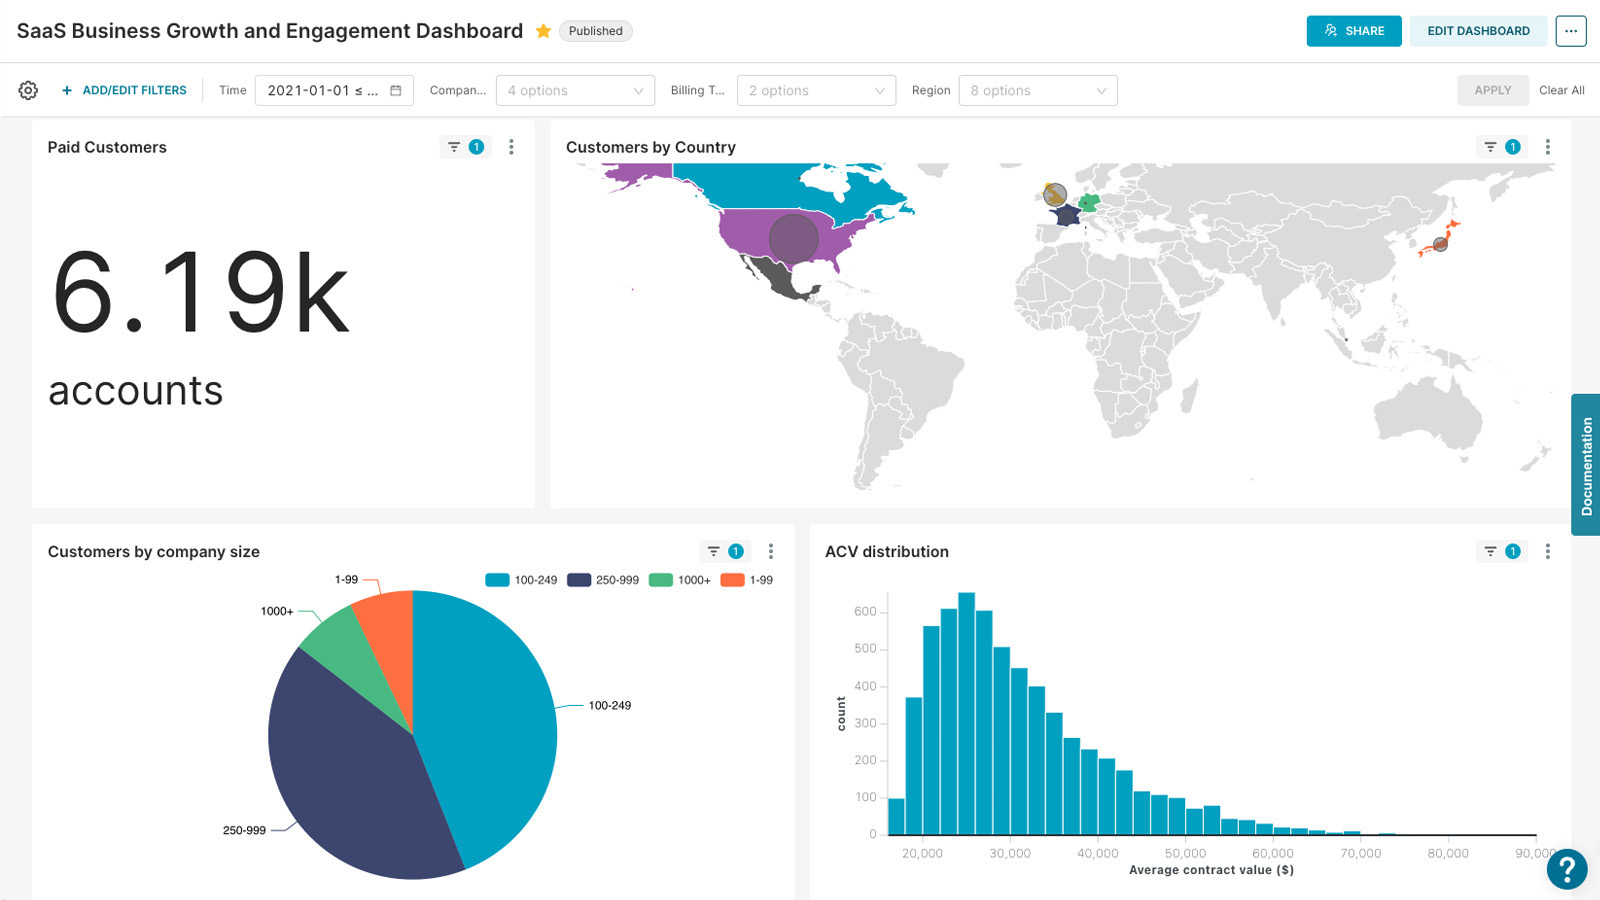
\includegraphics[width=0.9\textheight, angle=90]{figures/superset-dashboard.jpg}
    \caption{An example Apache Superset dashboard~\cite{ASF2024a}.}
    \label{fig:superset-dashboard}
\end{figure}

\begin{figure}[H]
    \centering
    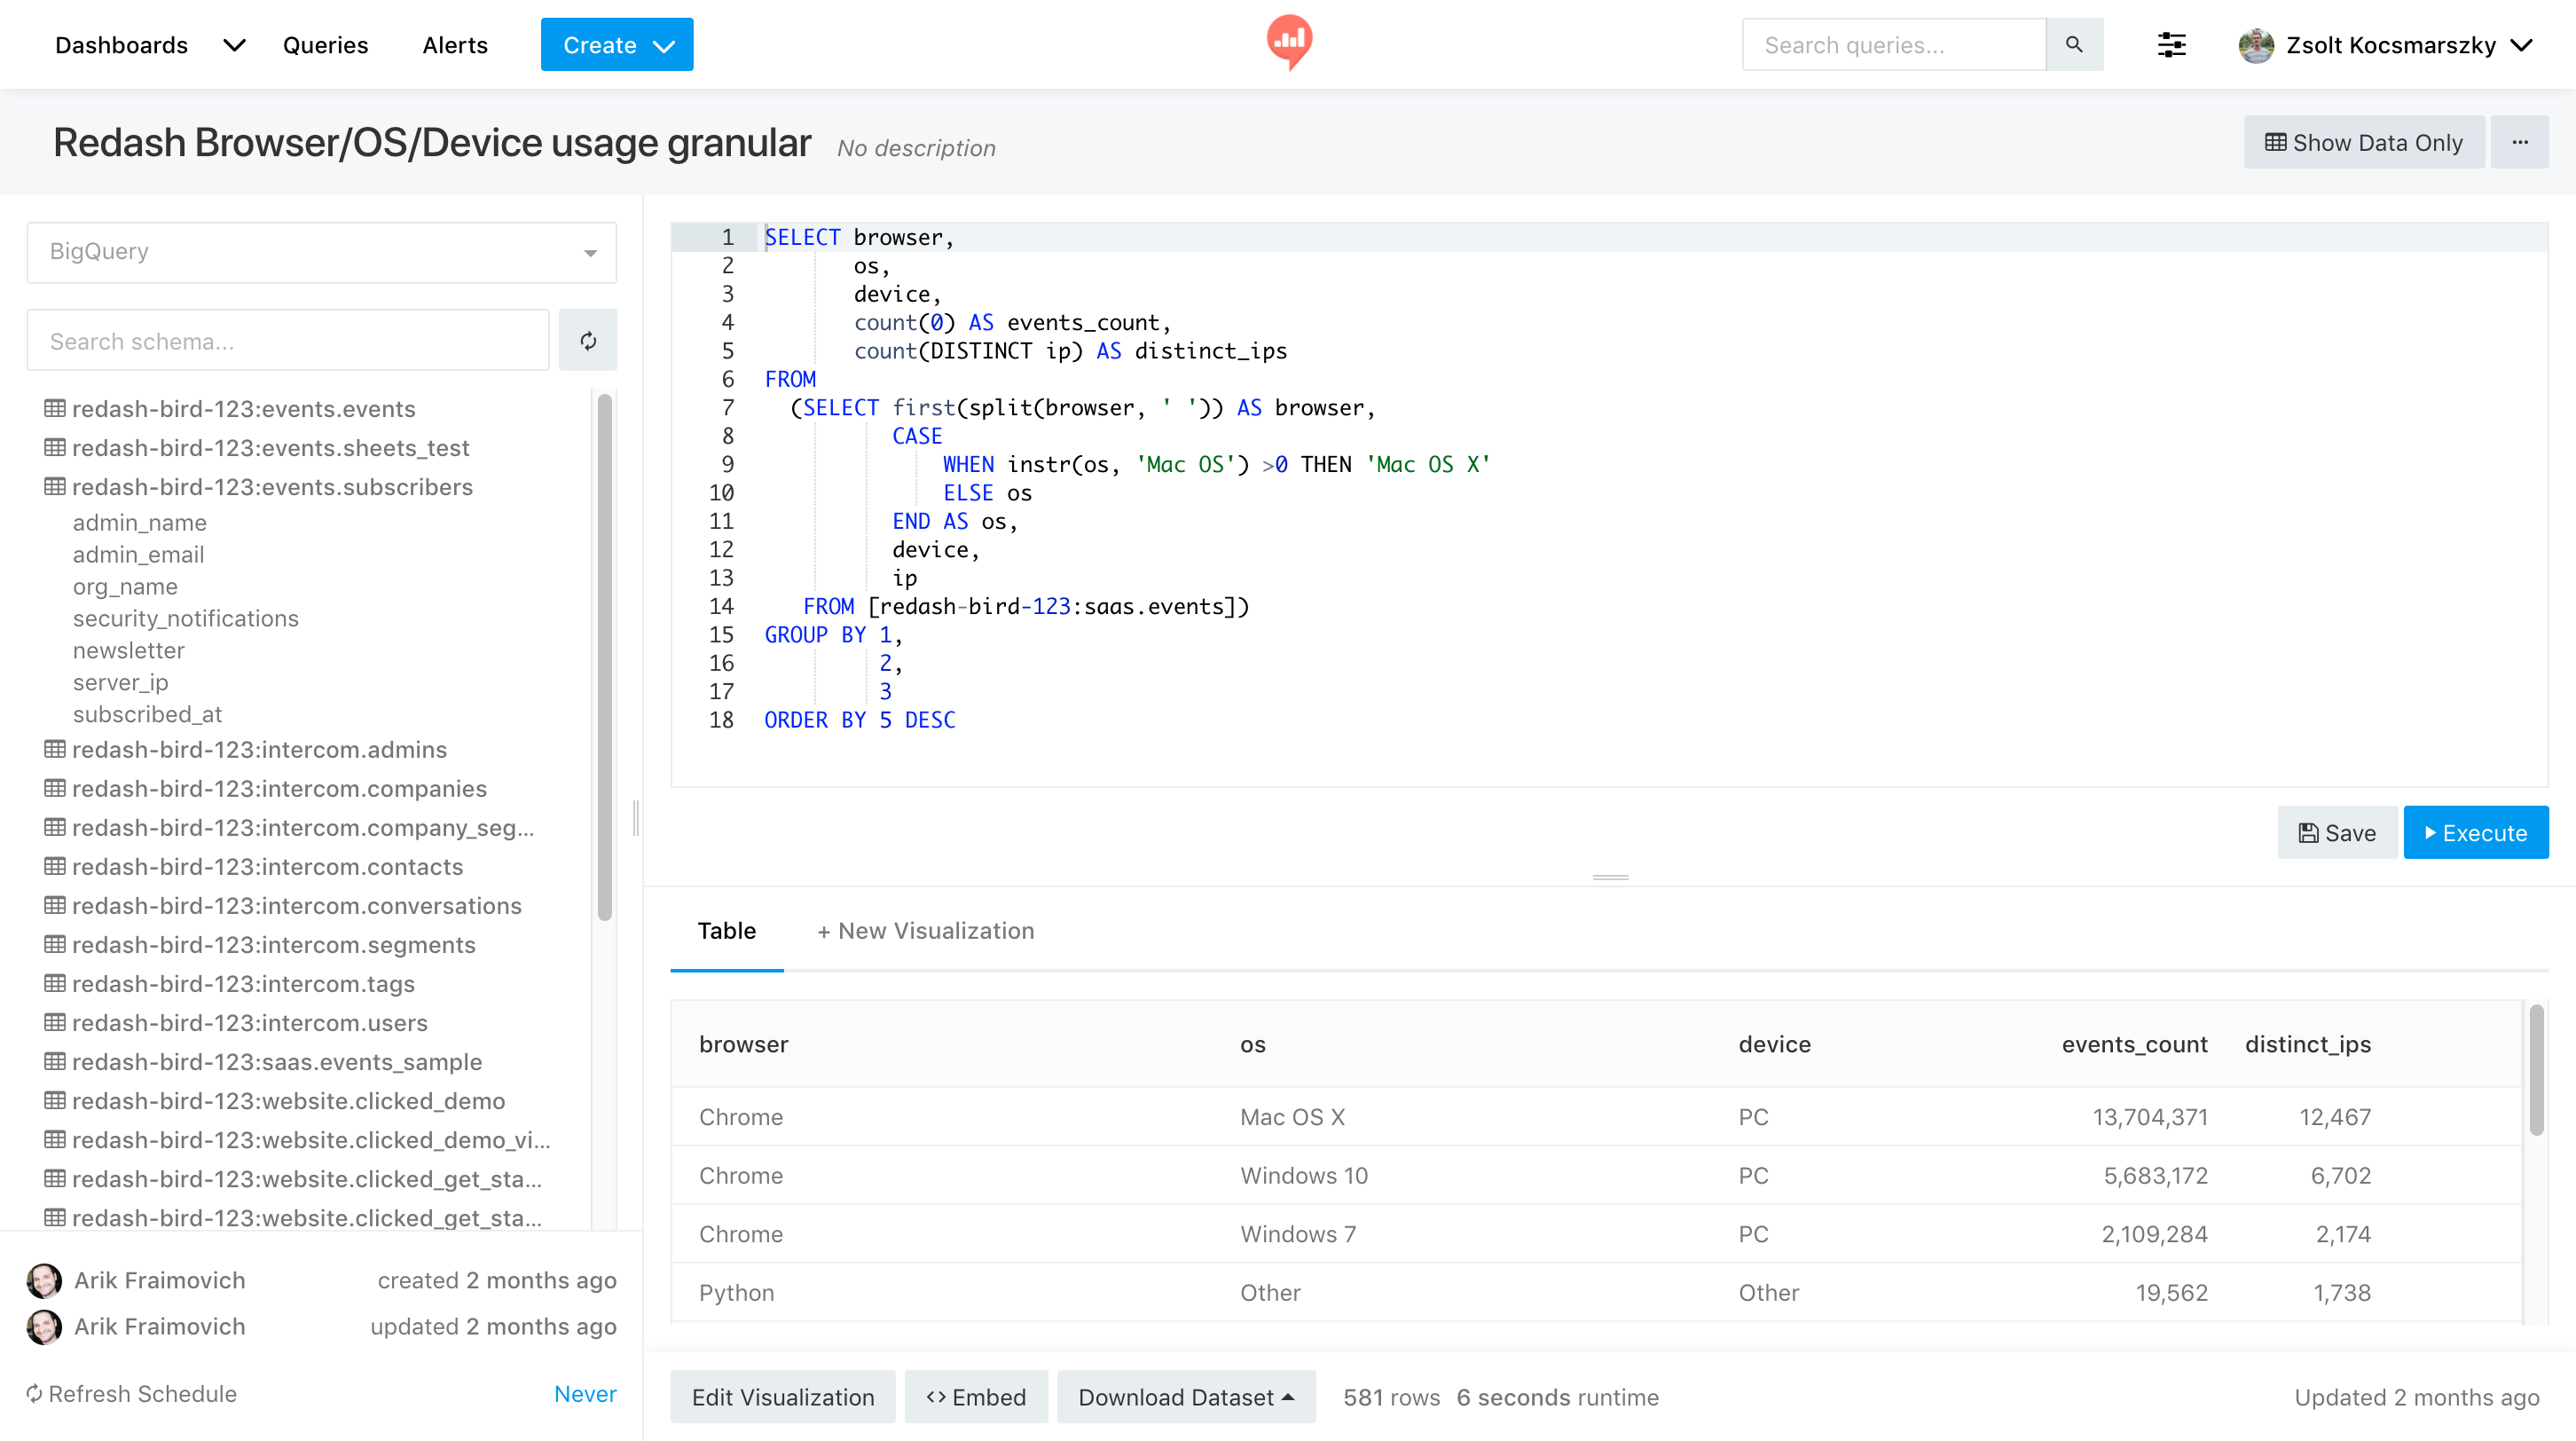
\includegraphics[width=0.9\textheight, angle=90]{figures/redash-query-editor.png}
    \caption{Redash's query editor~\cite{RedashCommunity2024}.}
    \label{fig:redash-query-editor}
\end{figure}

\begin{figure}[H]
    \centering
    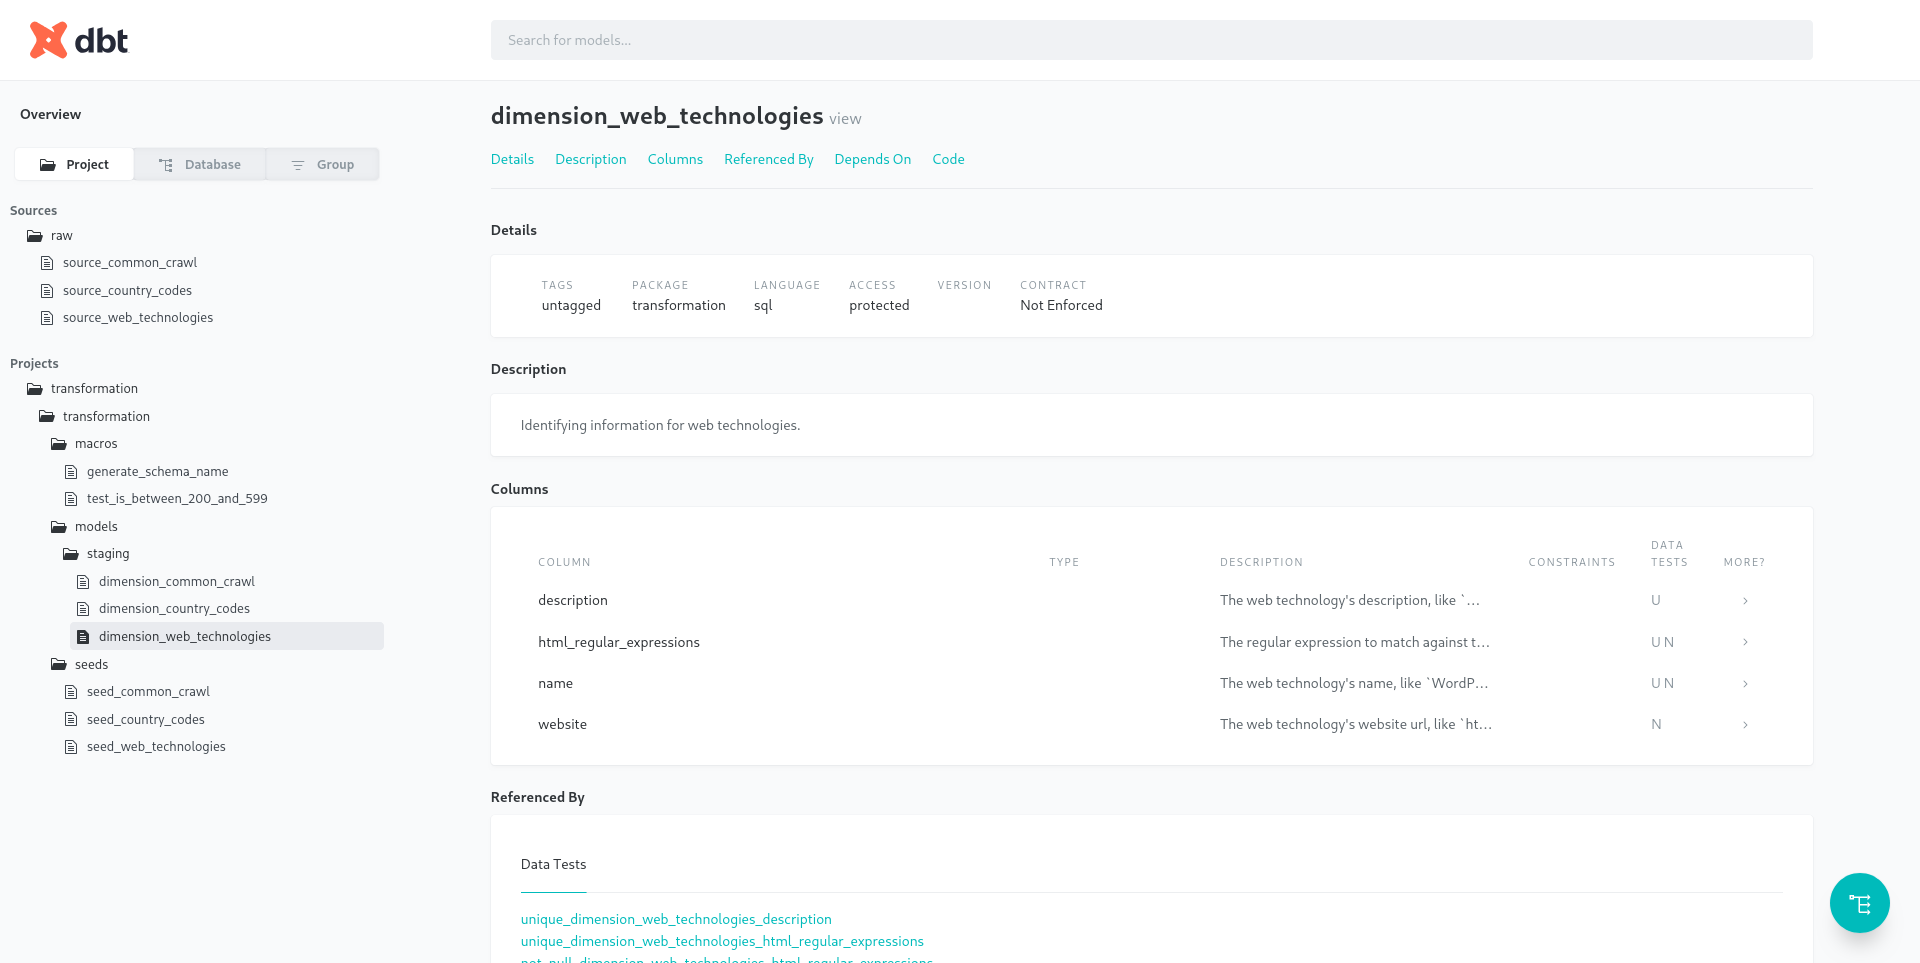
\includegraphics[width=0.9\textheight, angle=90]{figures/dbt-docs.png}
    \caption{Documentation of the dbt project.}
    \label{fig:appendix-guis-dbt-docs}
\end{figure}

\section{Local Kubernetes}
\label{sec:appendix-kubernetes}

Several Kubernetes distributions and virtualization environments support running Kubernetes locally.
\href{https://k3s.io/}{\textit{k3s}}, a certified Kubernetes distribution, is tailored for resource-constrained environments, which suits development contexts as opposed to multi-server production environments.
k3s can also run in Docker via a wrapper named \href{https://k3d.io/}{\textit{k3d}}.
The following command sets up a cluster with four namespaces in Kubernetes and a \href{https://traefik.io/traefik/}{\textit{Traefik}} ingress for external access to services:

\mint{sh}|k3d cluster create lakehouse|

Using the Kubernetes \ac{cli} \texttt{kubectl} and \href{https://helm.sh/}{\textit{Helm}} as the Kubernetes package manager, the installation of Longhorn (shown in \cref{lst:longhorn-setup}) fails.

\begin{listing}[H]
\begin{minted}{sh}
helm repo add longhorn https://charts.longhorn.io
helm repo update
helm install longhorn longhorn/longhorn --namespace longhorn-system --create-namespace
\end{minted}
\caption{Longhorn setup for Kubernetes using Helm.}
\label{lst:longhorn-setup}
\end{listing}

The issue arises because Longhorn relies on \ac{iscsi}, a protocol for connections and data transfers between computers and peripheral devices over \ac{tcp}, ``which cannot be installed in the standard k3s image, as it would have to use an OS base image''~\cite{Rizzi2021}.
According to a comment on the relevant feature request in k3d's \href{https://github.com/}{\textit{GitHub}} repository, creating a custom container image with a non-\texttt{scratch} OS base could resolve the issue.
However, this would be overly complex for our current needs.

Another local Kubernetes implementation is \href{https://minikube.sigs.k8s.io}{\textit{minikube}}, which can run on various drivers, including Docker and \acp{vm}.
To install the necessary \ac{iscsi} dependencies on an \ac{os}, we use the \ac{vm} driver as shown in \cref{lst:minikube-setup}.

\begin{listing}[H]
\begin{minted}{sh}
minikube start --driver=kvm2
minikube node add --worker
minikube ssh "sudo apt-get update;sudo apt-get install -y open-iscsi"
\end{minted}
\caption{Minikube setup using the VM driver.}
\label{lst:minikube-setup}
\end{listing}

Even though it is possible to install an \ac{iscsi} implementation, the service does not start, as \ac{iscsi} is also unsupported in minikube~\cite{Deutsch2017}.

The third and last option tested for a local Kubernetes setup was to use Rancher to create a Kubernetes cluster on Linux \acp{vm}.
Installing \texttt{open-iscsi} as above and deploying Longhorn through the Rancher \ac{gui} was initially successful.
However, issues arise when the cluster nodes reinitialize their availability, such as after waking from system hibernation, as Rancher becomes stuck waiting for the nodes to reconnect due to an ongoing bug~\cite{Henkens2023}.
This bug, opened in 2023, has since been closed due to inactivity.


\section{Supplementary Listings}
\label{sec:appendix-listings}

\begin{listing}[H]
\begin{minted}{bash}
#!/bin/bash
#
# Licensed to the Apache Software Foundation (ASF) under one
# or more contributor license agreements.  See the NOTICE file
# distributed with this work for additional information
# regarding copyright ownership.  The ASF licenses this file
# to you under the Apache License, Version 2.0 (the
# "License"); you may not use this file except in compliance
# with the License.  You may obtain a copy of the License at
#
#   http://www.apache.org/licenses/LICENSE-2.0
#
# Unless required by applicable law or agreed to in writing,
# software distributed under the License is distributed on an
# "AS IS" BASIS, WITHOUT WARRANTIES OR CONDITIONS OF ANY
# KIND, either express or implied.  See the License for the
# specific language governing permissions and limitations
# under the License.
set -e

start-master.sh -p 7077
# start-history-server.sh
start-thriftserver.sh  --driver-java-options "-Dderby.system.home=/tmp/derby"

# required for dbt
spark-sql <<EOF
CREATE DATABASE IF NOT EXISTS default;
EOF

# optional, to keep logs quiet
spark-sql <<EOF
CREATE DATABASE IF NOT EXISTS raw;
CREATE DATABASE IF NOT EXISTS staging;
CREATE DATABASE IF NOT EXISTS marts;
EOF

# Entrypoint, for example notebook, pyspark or spark-sql
if [[ $# -gt 0 ]] ; then
    eval "$1"
fi
\end{minted}
\caption{Entrypoint for the Spark master.}
\label{lst:spark-master-entrypoint}
\end{listing}

\begin{listing}[H]
\begin{minted}{bash}
#!/bin/bash
#
# Licensed to the Apache Software Foundation (ASF) under one
# or more contributor license agreements.  See the NOTICE file
# distributed with this work for additional information
# regarding copyright ownership.  The ASF licenses this file
# to you under the Apache License, Version 2.0 (the
# "License"); you may not use this file except in compliance
# with the License.  You may obtain a copy of the License at
#
#   http://www.apache.org/licenses/LICENSE-2.0
#
# Unless required by applicable law or agreed to in writing,
# software distributed under the License is distributed on an
# "AS IS" BASIS, WITHOUT WARRANTIES OR CONDITIONS OF ANY
# KIND, either express or implied.  See the License for the
# specific language governing permissions and limitations
# under the License.
set -e

pip install iso3166

start-worker.sh spark://spark-iceberg:7077 --port 8787
# start-history-server.sh

# Entrypoint, for example notebook, pyspark or spark-sql
if [[ $# -gt 0 ]] ; then
    eval "$1"
fi
\end{minted}
\caption{Entrypoint for a Spark worker.}
\label{lst:spark-worker-entrypoint}
\end{listing}

\begin{listing}[H]
\begin{minted}{bash}
#
# Licensed to the Apache Software Foundation (ASF) under one or more
# contributor license agreements.  See the NOTICE file distributed with
# this work for additional information regarding copyright ownership.
# The ASF licenses this file to You under the Apache License, Version 2.0
# (the "License"); you may not use this file except in compliance with
# the License.  You may obtain a copy of the License at
#
#    http://www.apache.org/licenses/LICENSE-2.0
#
# Unless required by applicable law or agreed to in writing, software
# distributed under the License is distributed on an "AS IS" BASIS,
# WITHOUT WARRANTIES OR CONDITIONS OF ANY KIND, either express or implied.
# See the License for the specific language governing permissions and
# limitations under the License.
#

# Default system properties included when running spark-submit.
# This is useful for setting default environmental settings.

spark.sql.extensions                        org.apache.iceberg.spark.extensions.IcebergSparkSessionExtensions
spark.sql.catalog.demo                      org.apache.iceberg.spark.SparkCatalog
spark.sql.catalog.demo.type                 rest
spark.sql.catalog.demo.uri                  http://rest:8181
spark.sql.catalog.demo.io-impl              org.apache.iceberg.aws.s3.S3FileIO
spark.sql.catalog.demo.s3.endpoint          http://minio:9000
spark.sql.catalog.demo.s3.path-style-access true
spark.sql.defaultCatalog                    demo
spark.eventLog.enabled                      true
spark.eventLog.dir                          /home/iceberg/spark-events
spark.history.fs.logDirectory               /home/iceberg/spark-events
spark.sql.catalogImplementation             in-memory
\end{minted}
\caption{Spark's default configuration.}
\label{lst:spark-defaults}
\end{listing}

\begin{listing}[H]
\begin{minted}{yaml}
services:
  minio:
    environment:
      MINIO_DOMAIN: minio
    networks:
      default:
        aliases:
        - lakehouse.minio
\end{minted}
\caption{Docker Compose configuration for MinIO's Virtual Host access style.}
\label{lst:compose-mino-virtual-host}
\end{listing}

\begin{listing}[H]
\begin{minted}{python}
@measure_performance
def fetch_warc_datasets():
  url = "https://index.commoncrawl.org/collinfo.json"
  response = requests.get(url)
  response.raise_for_status()
  datasets = response.json()

  if not datasets:
    raise ValueError("No datasets found.")

  return datasets


@measure_performance
def fetch_warc_paths(dataset_id: str, dataset_subset: str = 'warc'):
  url = urljoin(
    "https://data.commoncrawl.org/",
    f"crawl-data/{dataset_id}/{dataset_subset}.paths.gz",
  )
  response = requests.get(url)
  response.raise_for_status()

  warc_paths = (
    gzip.decompress(response.content)
    .decode("utf-8")
    .splitlines()
  )

  if not warc_paths:
    raise ValueError("No WARC paths found.")

  return warc_paths


@retry(
    stop=stop_after_attempt(5),
    wait=wait_exponential(min=1, max=10),
)
@measure_performance
def fetch_warc_stream(warc_file: str):
  url = urljoin("https://data.commoncrawl.org/", warc_file)
  response = requests.get(url, stream=True)
  response.raise_for_status()

  return response
\end{minted}
\caption{Network utility functions for Common Crawl ingestion.}
\label{lst:dagster-source-common-crawl-fetch}
\end{listing}


\begin{listing}[H]
\begin{minted}{python}
def measure_performance(func):
  def wrapper(*args, **kwargs):
    start_time = time.perf_counter()
    result = func(*args, **kwargs)
    end_time = time.perf_counter()
    elapsed_time = end_time - start_time
    logger.info(f"Time to execute {func.__name__}: {elapsed_time:.4f} seconds")
    return result

  return wrapper
\end{minted}
\caption{Decorator for performance measurement.}
\label{lst:dagster-utility-performance-measurement}
\end{listing}


\begin{listing}[H]
\begin{minted}{python}
def batch_records(
  data: Generator,
  max_batch_size=134217728, # bytes = 128 MiB
):
  counter = 0
  batch = []
  batch_size = 0

  for record in data:
    record_size = asizeof.asizeof(record)

    if batch_size + record_size > max_batch_size:
      if batch:
        yield batch
        batch = []
        batch_size = 0

    batch.append(record)
    batch_size += record_size
    counter += 1

  if batch:
    yield batch
\end{minted}
\caption{Batching algorithm for records up to a specified batch size.}
\label{lst:dagster-utility-performance-batching}
\end{listing}


\begin{listing}[H]
\begin{minted}{python}
BUFFER_SIZE = 5


async def batch_process(
  data_stream: Generator,
  func: Callable[[List[dict], bool], None]
):
  is_written = False
  buffer = asyncio.Queue(maxsize=BUFFER_SIZE)

  async def producer():
    for batch in data_stream:
      await buffer.put(batch)

    await buffer.put(None)

  async def fetch_next_item():
    try:
      batch = next(data_stream)
      await buffer.put(batch)
    except StopIteration:
      await buffer.put(None)

  async def consumer():
    nonlocal is_written
    while True:
      batch = await buffer.get()

      if batch is None:
        buffer.task_done()
        await buffer.put(None)
        break

      func(batch, is_written)

      if not is_written:
        is_written = True

      buffer.task_done()

      if buffer.qsize() < BUFFER_SIZE:
        await fetch_next_item()

  initial_fill = [fetch_next_item() for _ in range(BUFFER_SIZE)]
  await asyncio.gather(*initial_fill)
  await consumer()
\end{minted}
\caption{Queuing algorithm for processing batches with a specified buffer size.}
\label{lst:dagster-utility-performance-queuing}
\end{listing}

\begin{listing}[H]
\begin{minted}{python}
MEMORY = "50g" if IS_KUBERNETES else "4g"


class SparkSingleton:
  def __init__(self):
    self._spark = None

  @property
  def spark(self):
    if self._spark is None:
      self._spark = (
        SparkSession.builder.appName("Big Data Pipeline")
        .master("spark://spark-iceberg:7077")
        .config("spark.driver.host", "dagster")
        .config("spark.driver.bindAddress", "0.0.0.0")
        .config("spark.driver.memory", MEMORY)
        .config("spark.driver.port", "7777")
        .config("spark.blockManager.port", "7878")
        .config("spark.executor.memory", MEMORY)
        .config("spark.rpc.message.maxSize", "1024")
        .config(
          "spark.jars.packages",
          "org.apache.iceberg:iceberg-spark-runtime-3.5_2.12:1.6.1,"
          "org.apache.iceberg:iceberg-aws-bundle:1.6.1",
        )
        .config(
          "spark.sql.extensions",
          "org.apache.iceberg.spark.extensions.IcebergSparkSessionExtensions",
        )
        .config("spark.sql.catalog.demo", "org.apache.iceberg.spark.SparkCatalog")
        .config("spark.sql.catalog.demo.type", "rest")
        .config("spark.sql.catalog.demo.uri", "http://rest:8181")
        .config("spark.sql.catalog.demo.io-impl", "org.apache.iceberg.aws.s3.S3FileIO")
        .config("spark.sql.catalog.demo.s3.endpoint", "http://minio:9000")
        .config("spark.sql.catalog.demo.s3.path-style-access", "true")
        .config("spark.sql.defaultCatalog", "demo")
        .config("spark.sql.catalogImplementation", "in-memory")
        .getOrCreate()
      )
    return self._spark


SparkManager = SparkSingleton()
\end{minted}
\caption{\texttt{SparkSession} defined as a singleton.}
\label{lst:dagster-utility-spark}
\end{listing}

\begin{listing}[H]
\begin{minted}{python}
TABLE = "raw.source_common_crawl"


def write_source(batch: list):
  if not SparkManager.spark.catalog.tableExists(TABLE):
    SparkManager.spark.sql(f"""
      CREATE TABLE {TABLE} (
        dataset_id string NOT NULL,
        response_charset string,
        response_headers_status_code integer NOT NULL,
        response_payload string NOT NULL,
        response_payload_size_bytes integer NOT NULL,
        response_payload_length integer NOT NULL,
        response_target_uri string NOT NULL
      )
      USING iceberg
      PARTITIONED BY (dataset_id, response_charset)
    """)
    SparkManager.spark.sql(
      f"ALTER TABLE {TABLE} SET IDENTIFIER FIELDS dataset_id, response_target_uri"
    )

  dataframe = SparkManager.spark.createDataFrame(batch)
  existing_data = SparkManager.spark.table(TABLE)
  new_rows = dataframe.join(
    existing_data,
    on=(dataframe["dataset_id"] == existing_data["dataset_id"])
    & (dataframe["response_target_uri"] == existing_data["response_target_uri"]),
    how="left_anti",
  )
  new_rows.writeTo(TABLE).append()
\end{minted}
\caption{Appending deduplicated entries to a partitioned Iceberg table.}
\label{lst:dagster-source-common-crawl-write-deduplicated}
\end{listing}

\begin{listing}[H]
\begin{minted}{jinja}

Data from one of the largest public web crawling datasets.



The HTTP status code of the response, such as `200`.

\end{minted}
\caption{Definition of documentation in dbt.}
\label{lst:appendix-listings-dbt-doc}
\end{listing}

\begin{listing}[H]
\begin{minted}{sh}
poetry run dbt docs generate
poetry run dbt docs serve
\end{minted}
\caption{Commands to generate and serve dbt project documentation.}
\label{lst:implementation-pipeline-transformation-dbt-docs}
\end{listing}

\begin{listing}[H]
\begin{minted}{python}
COUNTRY_CODES_URL = "https://en.wikipedia.org/wiki/List_of_ISO_3166_country_codes"
MODULE_NAME = "country_codes"


def fetch_tables() -> list[pandas.DataFrame]:
  # without `keep_default_na`, the country code for Namibia (`NA`) would be parsed as `NoneType`
  tables = pandas.read_html(COUNTRY_CODES_URL, keep_default_na=False)
  return tables
\end{minted}
\caption{Basic table extraction using Pandas.}
\label{lst:appendix-listings-pandas-tables}
\end{listing}

\begin{listing}[H]
\begin{minted}{bash}
FROM python:3.11.9 AS base-image
ENV CI=true
ENV PYTHONUNBUFFERED=1
ENV DAGSTER_HOME=/home/rootless/dagster
WORKDIR /srv/app/
# ... install poetry, add user `rootless` ...
USER rootless:rootless
RUN mkdir /home/rootless/dagster \
  && touch /home/rootless/dagster/dagster.yaml \
  && poetry config virtualenvs.in-project true

FROM base-image AS development
COPY ./docker/dagster/entrypoint.sh /usr/local/bin/docker-entrypoint.sh
ENTRYPOINT ["docker-entrypoint.sh"]
CMD ["poetry", "run", "dagster", "dev", "--host", "0.0.0.0"]
VOLUME /srv/app
VOLUME /srv/charts
VOLUME /srv/transformation
EXPOSE 3000

FROM base-image AS prepare
COPY --chown=rootless ./orchestration/pyproject.toml ./orchestration/poetry.lock ./orchestration/
WORKDIR /srv/app/orchestration
RUN poetry install

FROM prepare AS build
WORKDIR /srv/app
COPY --chown=rootless ./orchestration ./orchestration
COPY --chown=rootless ./transformation ./transformation
WORKDIR /srv/app/orchestration
RUN poetry run dagster-dbt project prepare-and-package --file orchestration/project.py

FROM build AS production
ENV DAGSTER_DEPLOYMENT=production
USER root:root
# ... install updates ...
USER rootless:rootless
CMD ["poetry", "run", "dagster-webserver", "--host", "0.0.0.0"]
VOLUME /srv/charts
EXPOSE 3000
\end{minted}
\caption{Multistage Dockerfile for the Big Data pipeline.}
\label{lst:appendix-listings-dockerfile}
\end{listing}

\begin{listing}[H]
\begin{minted}{text}
INFO:root:Time to execute fetch_warc_datasets: 0.3882 seconds
INFO:root:Time to execute fetch_warc_paths: 0.1251 seconds
INFO:root:Processing path "crawl-data/CC-MAIN-2024-42/segments/1727944253146.59/warc/ CC-MAIN-20241003094020-20241003124020-00000.warc.gz"
INFO:root:Time to execute fetch_warc_stream: 0.6644 seconds
INFO:root:Time to execute get_warc_record_stream: 0.0000 seconds
org.apache.iceberg#iceberg-spark-runtime-3.5_2.12 added as a dependency
org.apache.iceberg#iceberg-aws-bundle added as a dependency
:: resolving dependencies :: org.apache.spark#spark-submit-parent-6ac38175-0b5c-4e68-a308-36539b91fc31; 1.0
    confs: [default]
    found org.apache.iceberg#iceberg-spark-runtime-3.5_2.12;1.6.1 in central
    found org.apache.iceberg#iceberg-aws-bundle;1.6.1 in central
:: resolution report :: resolve 174ms :: artifacts dl 6ms
    :: modules in use:
    org.apache.iceberg#iceberg-aws-bundle;1.6.1 from central in [default]
    org.apache.iceberg#iceberg-spark-runtime-3.5_2.12;1.6.1 from central in [default]
    ---------------------------------------------------------------------
    |                  |            modules            ||   artifacts   |
    |       conf       | number| search|dwnlded|evicted|| number|dwnlded|
    ---------------------------------------------------------------------
    |      default     |   2   |   0   |   0   |   0   ||   2   |   0   |
    ---------------------------------------------------------------------
:: retrieving :: org.apache.spark#spark-submit-parent-6ac38175-0b5c-4e68-a308-36539b91fc31
    confs: [default]
    0 artifacts copied, 2 already retrieved (0kB/6ms)
WARN TaskSetManager: Stage 0 contains a task of very large size (3827 KiB).  The maximum recommended task size is 1000 KiB.
INFO:root:Time to execute write_source: 68.0258 seconds
WARN TaskSetManager: Stage 6 contains a task of very large size (3182 KiB).  The maximum recommended task size is 1000 KiB.
INFO:root:Time to execute write_source: 42.6831 seconds
WARN TaskSetManager: Stage 12 contains a task of very large size (2918 KiB). The maximum recommended task size is 1000 KiB.
INFO:root:Time to execute write_source: 38.4028 seconds
WARN TaskSetManager: Stage 18 contains a task of very large size (3283 KiB). The maximum recommended task size is 1000 KiB.
INFO:root:Time to execute write_source: 37.8254 seconds
# ...
WARN TaskSetManager: Stage 48 contains a task of very large size (1679 KiB). The maximum recommended task size is 1000 KiB.
INFO:root:Time to execute write_source: 35.3250 seconds
\end{minted}
\caption{Simplified asset job logs for Common Crawl ingestion.}
\label{lst:appendix-listings-spark-logs}
\end{listing}


\clearpage
\section{Spark Driver}
\label{sec:appendix-spark}

\begin{figure}[H]
    \centering
    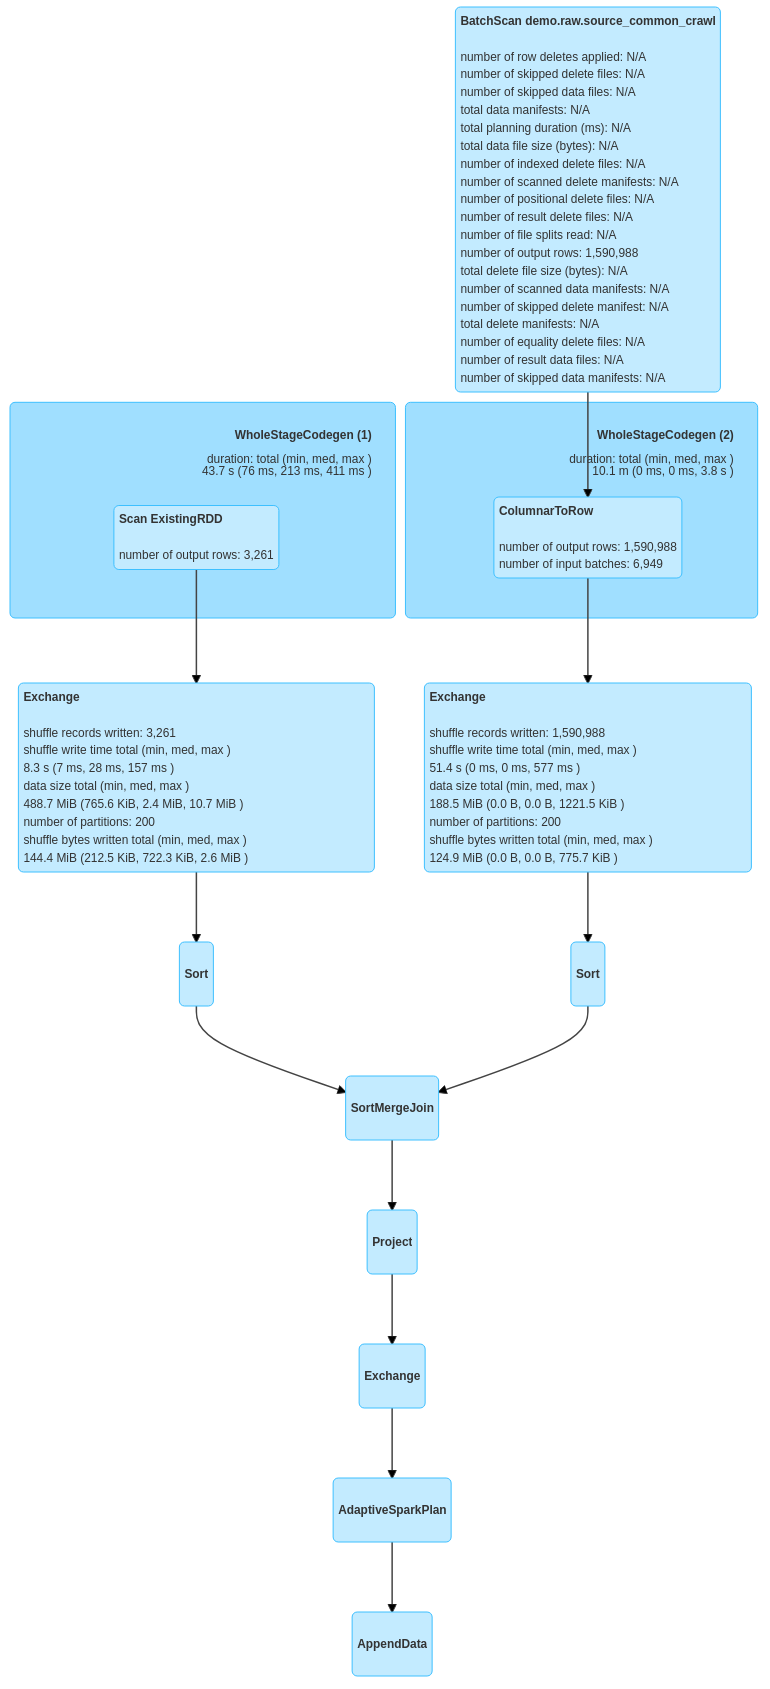
\includegraphics[height=0.9\textheight]{figures/driver-query.png}
    \caption{Spark driver's query diagram for appending data.}
    \label{fig:analysis-pipeline-performance-driver}
\end{figure}


\clearpage
\section{Overall Port List}
\label{sec:appendix-ports}

\begin{table}[H]
    \centering
    \begin{tabular}{|c|c|c|c|}
    \hline
    \textbf{Port} & \textbf{Application} & \textbf{Type} & \textbf{Component} \\
    \hline
    3000 & Dagster & GUI & ~ \\
    \hline
    3001 & Charts & GUI & ~ \\
    \hline
    4040 & Spark & GUI & Driver \\
    \hline
    7077 & Spark & API & Master \\
    \hline
    7777 & Spark & API & Driver \\
    \hline
    7878 & Spark & API & Block Manager \\
    \hline
    8080 & Jupyter Notebook & GUI & ~ \\
    \hline
    8181 & Iceberg & API & REST Catalog \\
    \hline
    8888 & Spark & GUI & Master \\
    \hline
    9000 & MinIO & API & ~ \\
    \hline
    9001 & MinIO & GUI & ~ \\
    \hline
    10000 & Thrift & API & ~ \\
    \hline
    \end{tabular}
    \caption{List of ports and their respective applications.}
    \label{tab:appendix-ports}
\end{table}


\clearpage
\section{Large Charts}
\label{sec:appendix-charts}

\begin{figure}[H]
    \centering
    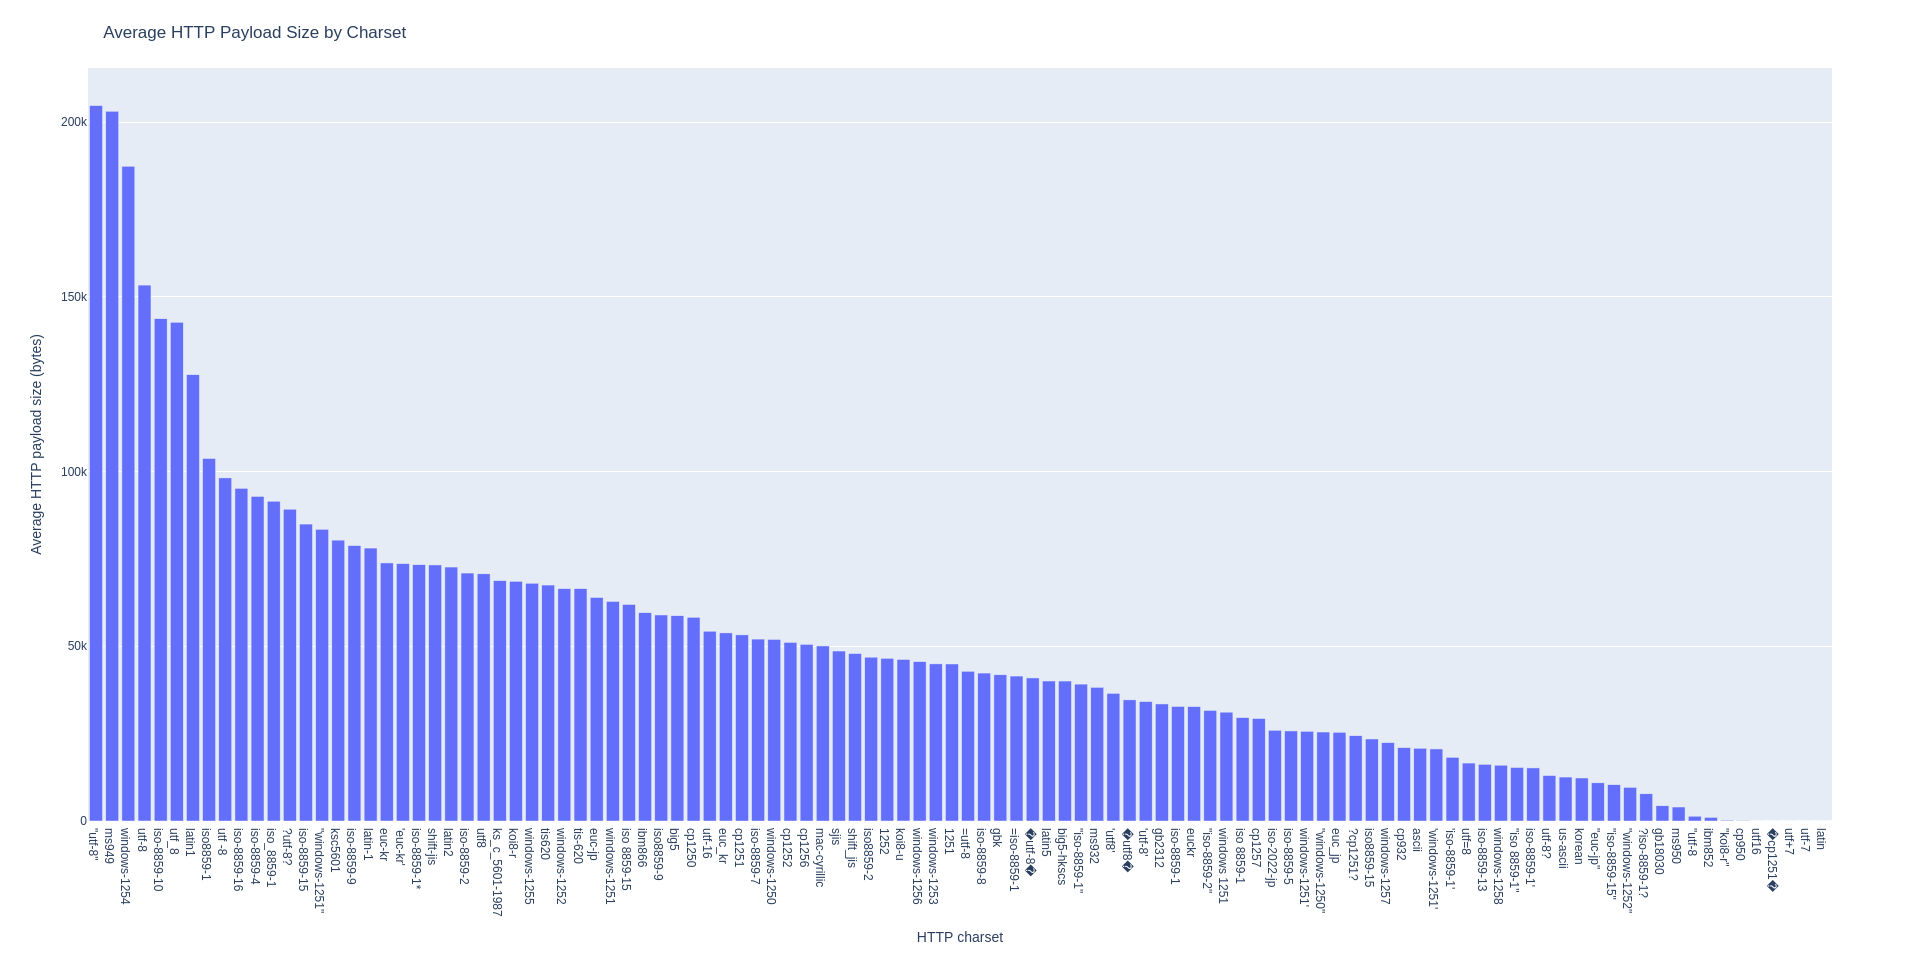
\includegraphics[width=0.9\textheight, angle=90]{figures/charts/large/appendix/chart_source_charset_bar_payload_size.png}
    \caption{Average payload size by charset.}
    \label{fig:analysis-dataset-chart_source_charset_bar_payload_size}
\end{figure}

\begin{figure}[H]
    \centering
    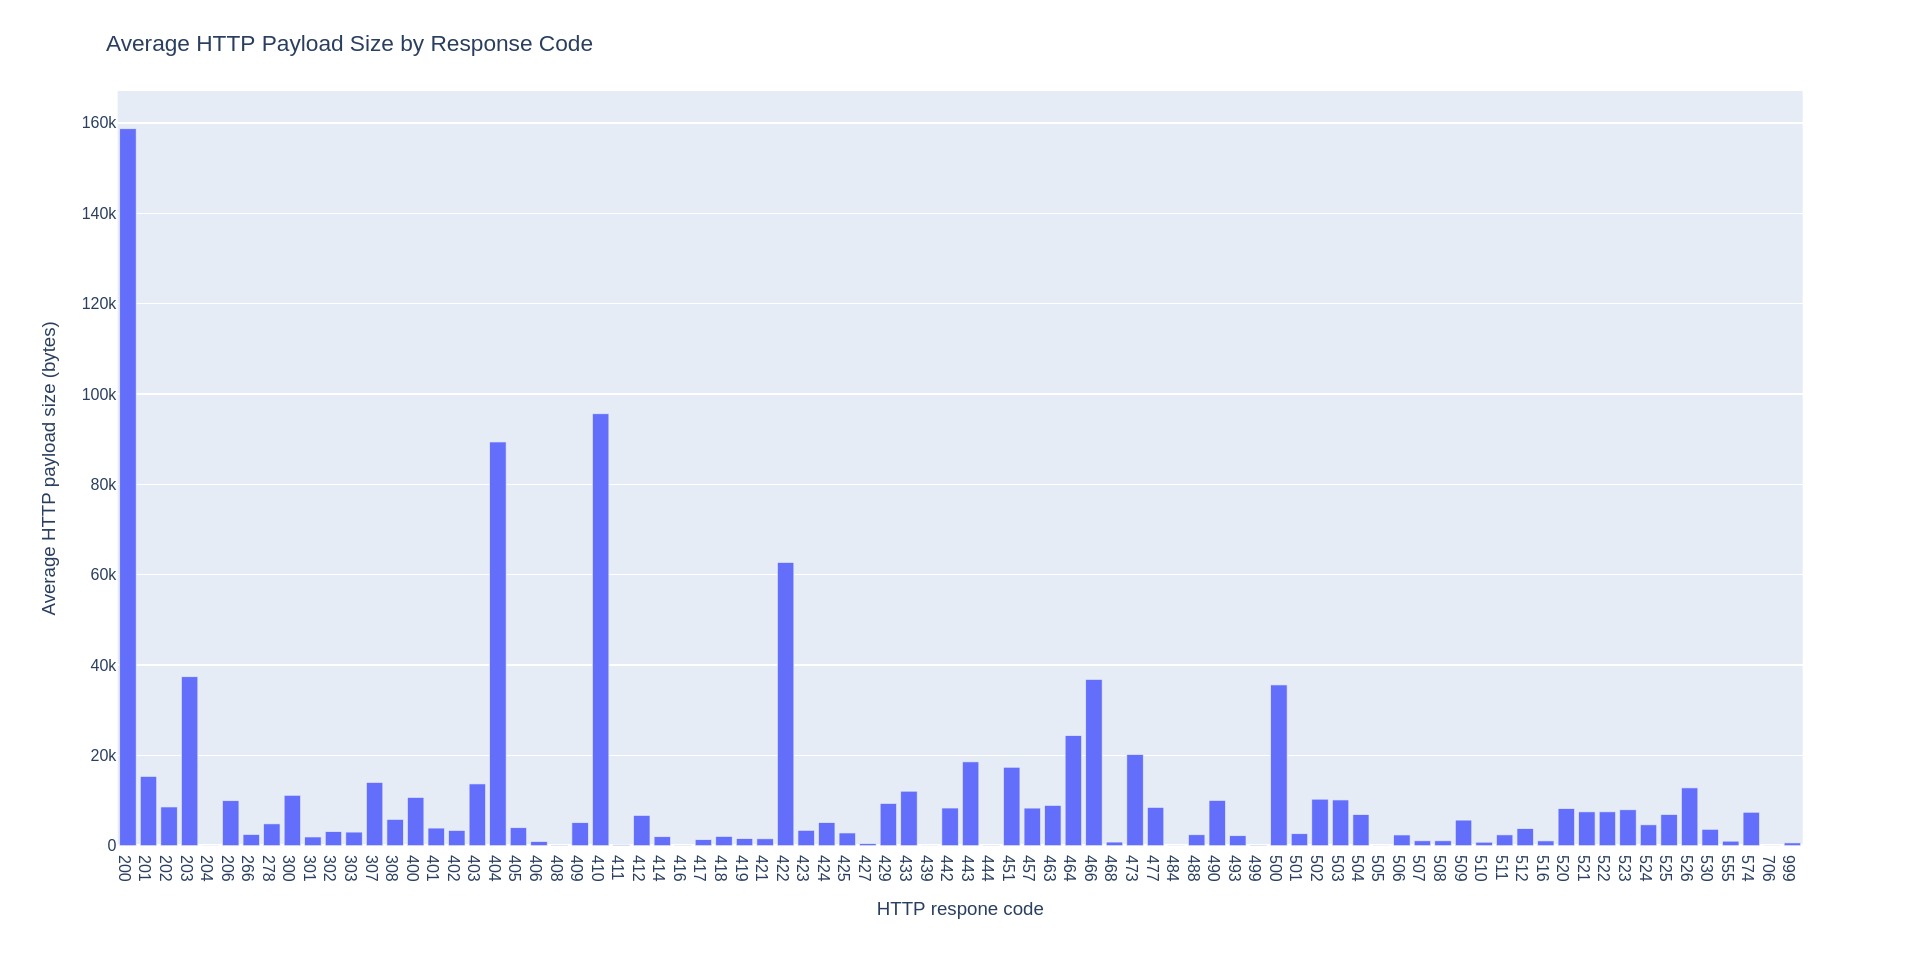
\includegraphics[width=\textheight, angle=90]{figures/charts/large/appendix/chart_source_response_code_bar_payload_size.png}
    \caption{Average payload size by response code.}
    \label{fig:analysis-dataset-chart_source_response_code_bar_payload_size}
\end{figure}

\begin{figure}[H]
    \centering
    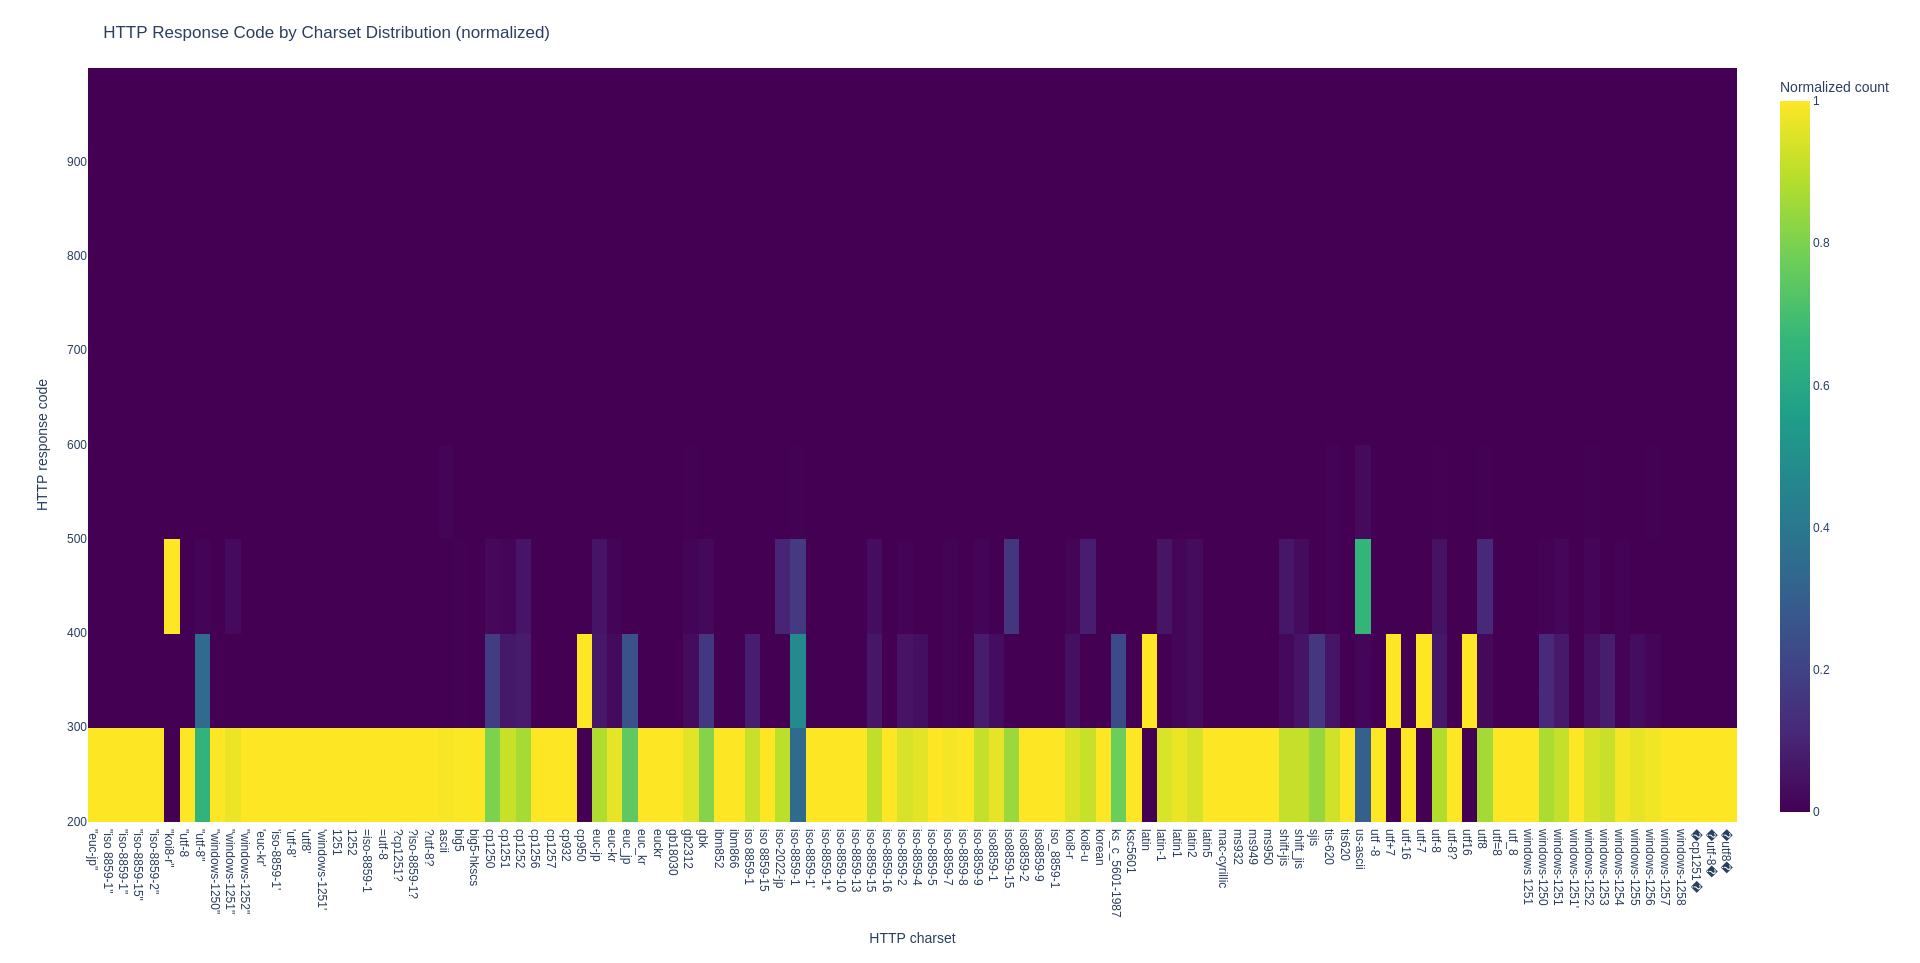
\includegraphics[width=\textheight, angle=90]{figures/charts/large/appendix/chart_source_charset_heatmap_response_code.png}
    \caption{Normalized response code distribution by charset.}
    \label{fig:analysis-dataset-chart_source_charset_heatmap_response_code}
\end{figure}

\begin{figure}[H]
    \centering
    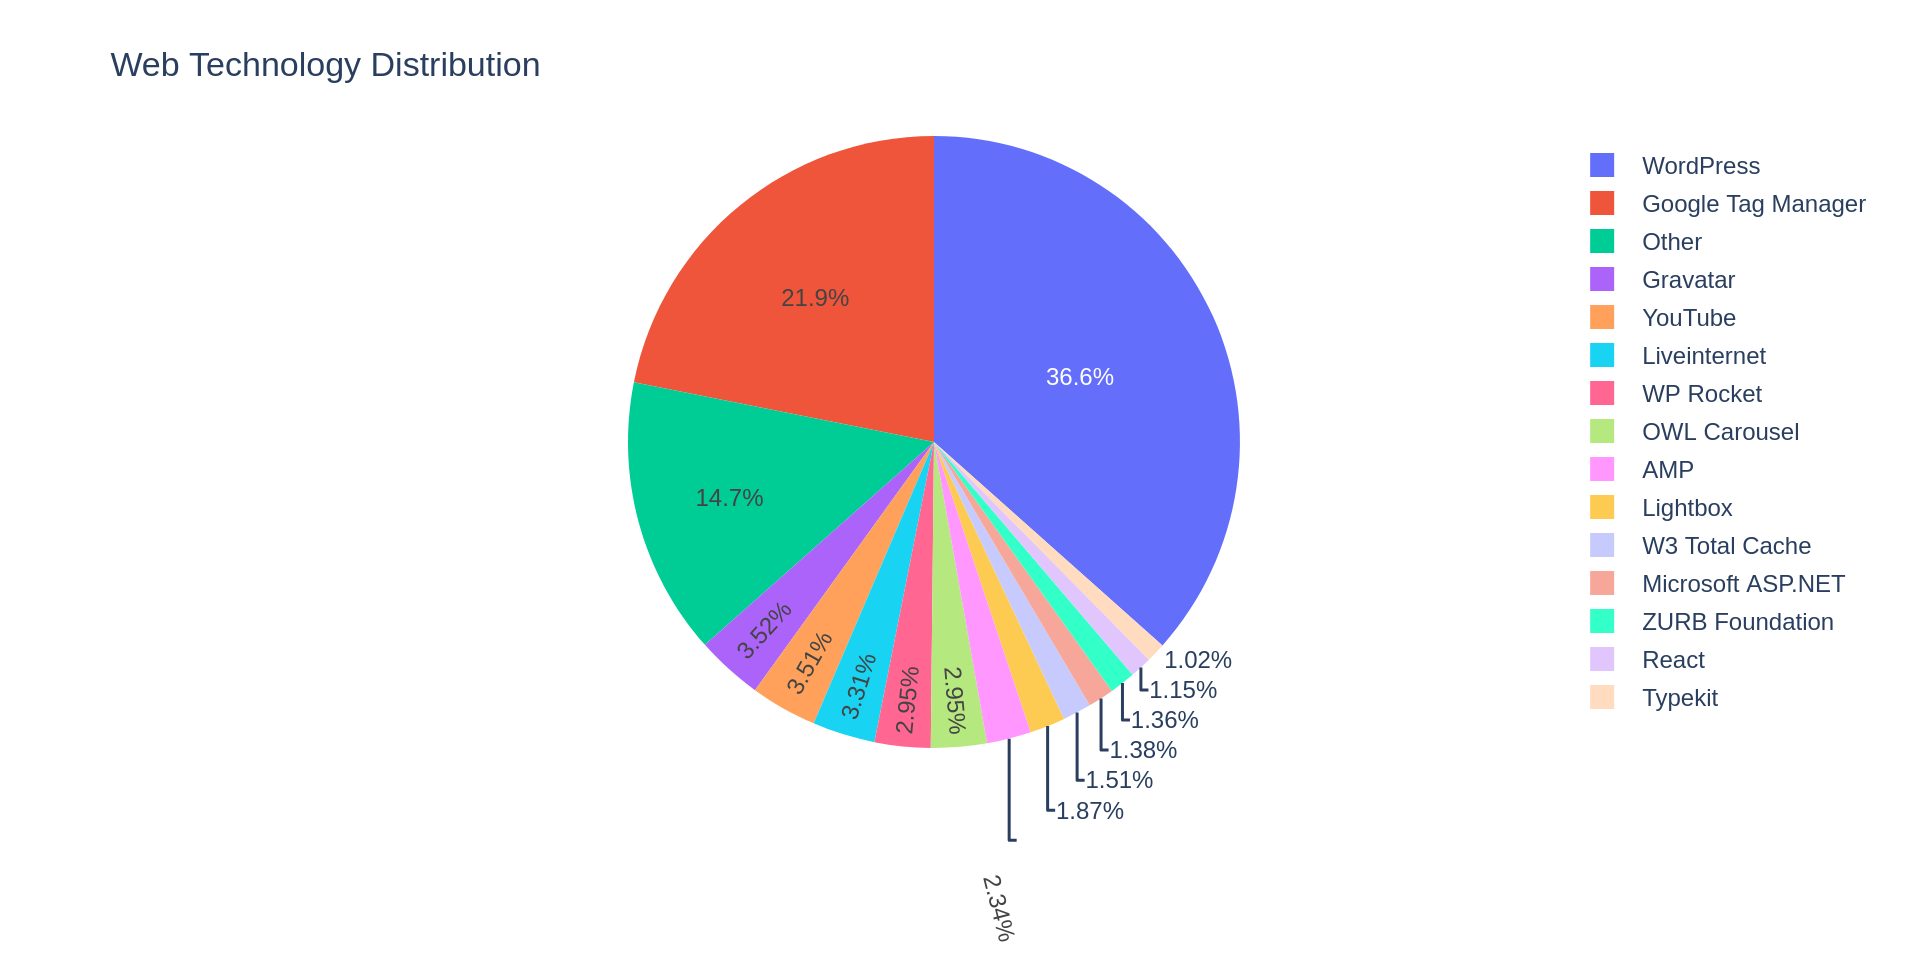
\includegraphics[width=\textheight, angle=90]{figures/charts/large/appendix/chart_fact_web_technology_pie.png}
    \caption{Distribution of web technologies.}
    \label{fig:analysis-dataset-chart_fact_web_technology_pie}
\end{figure}

\begin{figure}[H]
  \centering
  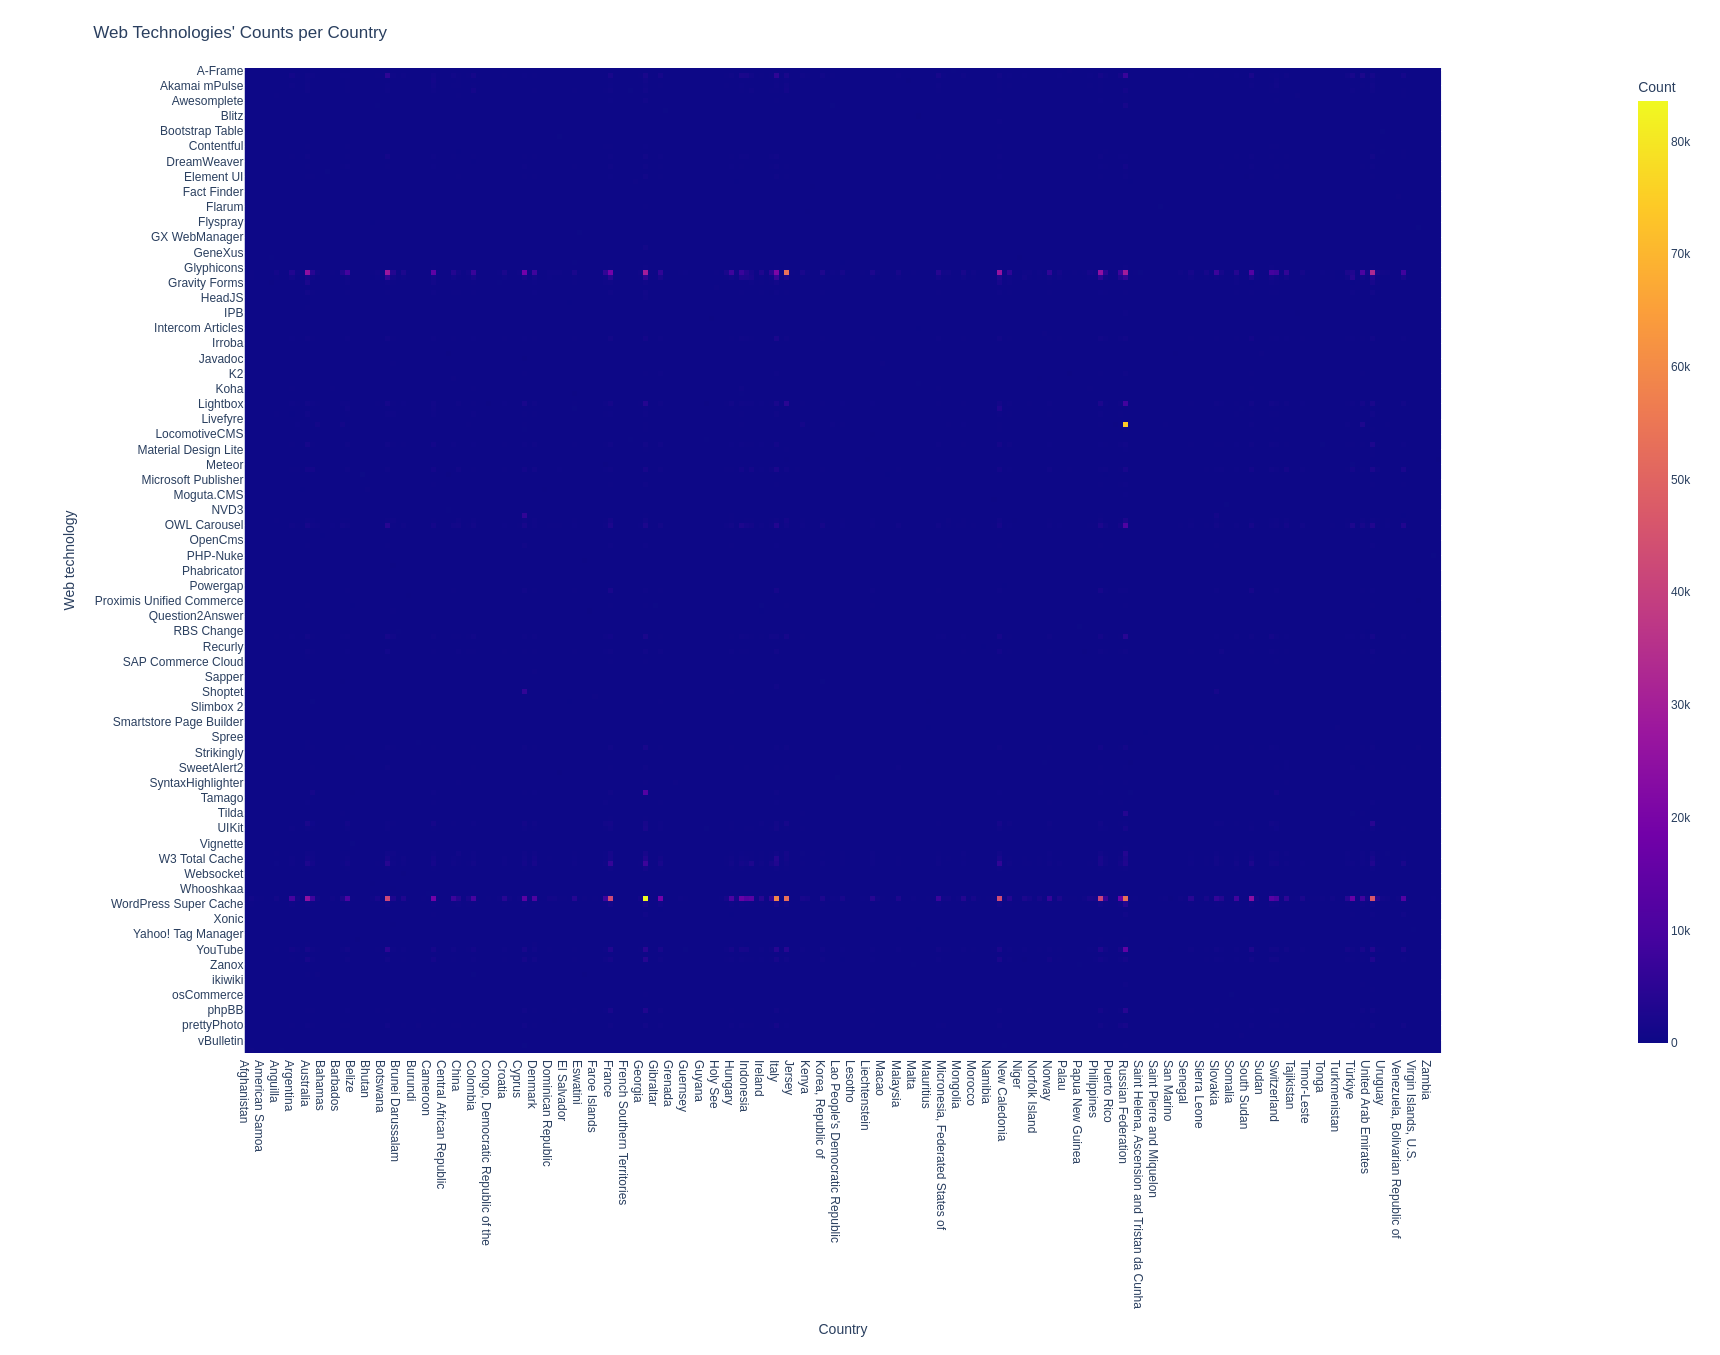
\includegraphics[height=\textwidth, angle=90]{figures/charts/large/appendix/chart_fact_web_technology_heatmap_country.png}
  \caption{Web technologies count per country.}
  \label{fig:analysis-dataset-chart_fact_web_technology_heatmap_country}
\end{figure}

\begin{figure}[H]
  \centering
  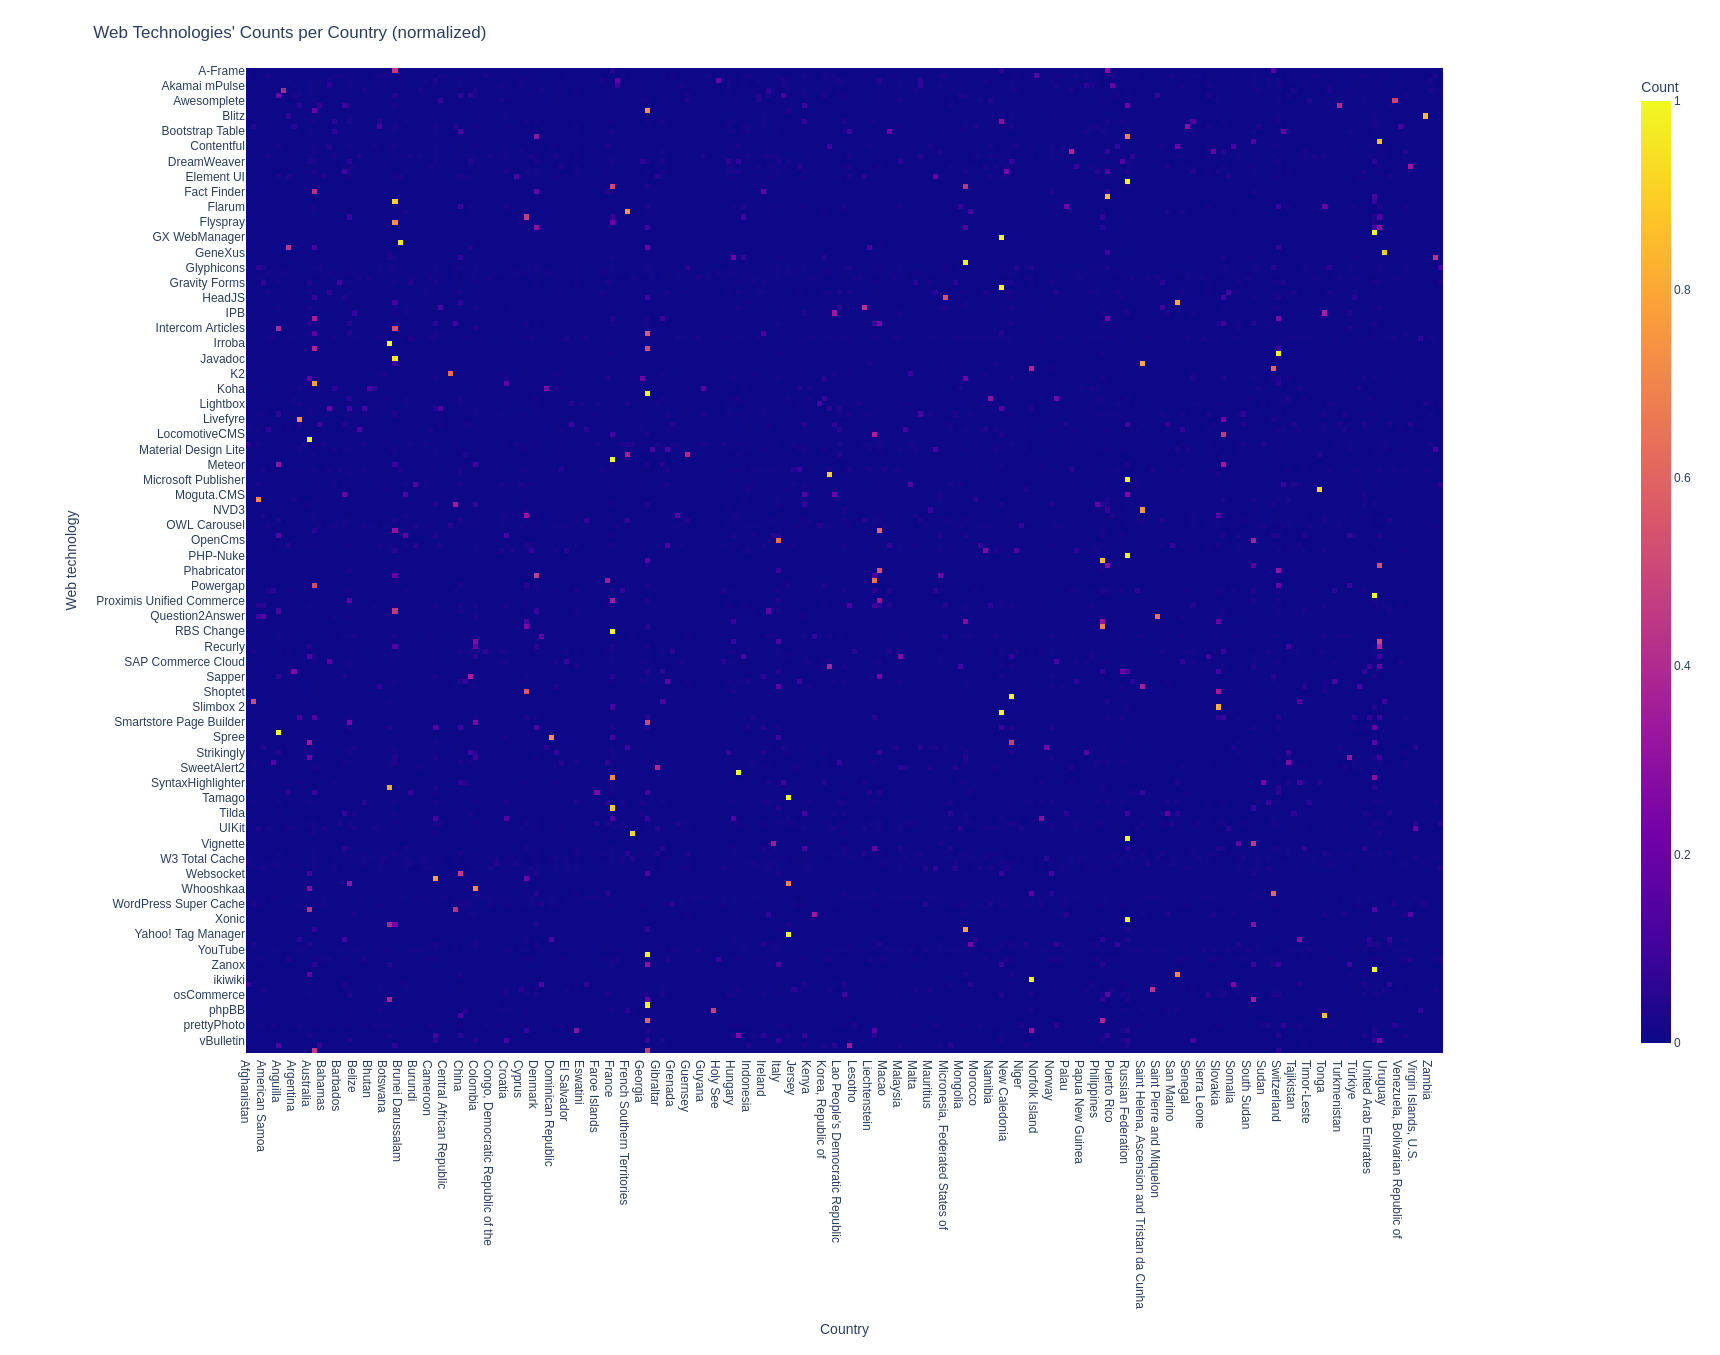
\includegraphics[height=\textwidth, angle=90]{figures/charts/large/appendix/chart_fact_web_technology_heatmap_country_normalized.png}
  \caption{Normalized web technologies count per country.}
  \label{fig:analysis-dataset-chart_fact_web_technology_heatmap_country_normalized}
\end{figure}


\newpage
\cleardoublepage
\section*{Statutory Declaration}
\thispagestyle{empty}
The author declares that he has written the thesis at hand independently, without outside help and without the use of any other but the listed sources. Thoughts taken directly or indirectly from external sources (including electronic sources) are marked accordingly without exception. Sources used verbatim and contentual were quoted according to the recognised rules for scientific working. This thesis has not been submitted in the same or similar form, not even partially, within the scope of a different examination.\\\\
Thus far it also has not been publicised yet.\\\\
I herewith agree that the thesis will be examined for plagiarism with the help of a plagiarism-detection service.\\\\\\
\noindent\rule{5cm}{.4pt}\hfill\rule{5cm}{.4pt}\par
\noindent Place, Date \hfill Signature of the author

\end{document}
